% PARTS OF THE THESIS WHICH ARE COMMENTED OUT ONLY FOR SHORTNESS DURING WRITING PROCESS BUT HAVE TO BE INCLUDED LATER ARE COMMENTED OUT WITH "%blubb"
% ALSO STUFF ONE HAS TO BE CAREFUL WITH IS COMMENTED WITH blubb


\documentclass[nativefonts,print]{Style/class_dissertation}


%%%%%%%%%%%%%%%%%%%%%%%%%%%%%%%%%%%%%%%%%%%%%%%%%%%%%%%%%%%%%%%%%%
% Stuff added by MW
%\newcommand{\red}[1]{\textcolor{red}{#1}}
	% This can be found in the PackagesNewCommands directory+file
%%%%%%%%%%%%%%%%%%%%%%%%%%%%%%%%%%%%%%%%%%%%%%%%%%%%%%%%%%%%%%%%%%

% load a collection of convenient shortcut commands


% Written by Noreen Walker,
% see also Thesis\Commands\additional_custom_commands
% For additional code by MW


% Define new convenient shortcut commands and include packages

% *******************************************
% include extrapackages
% *******************************************
\usepackage{soul}				% yellow highlighting \hl{}
\usepackage{textgreek}			%greek upright letters in text mode
\usepackage{xifthen}			%if statements, optional arguments in newcommand
\usepackage[export]{adjustbox}  %align images withing figure environment (left,right)
%\usepackage{endnotes}			%doesn't really work
\usepackage{placeins}			% prevent floats from floating behind the chapter end 	
%\usepackage{booktabs}			% nicer tables
\usepackage{tabu}				% thick lines in tables
\usepackage{colortbl}			% colored cells in tables
\usepackage{bm}					% bold math symbols
\usepackage{mdwlist}			% compact (itemize) lists: itemize*
\usepackage{float}				% enforce float-figure position, e.g. [H]
\usepackage{xfrac}				% small (inline) fractions (\sfrac)

% *******************************************
% Layout
% *******************************************
\renewcommand{\footnotesize}{\small}	% change footnotesize (increase to "small")
\newcommand{\defaultlinesep}{\tabulinesep = 0.8mm} % define a height separation for tables (tabu package)
\newcommand{\cellgray}{\cellcolor[rgb]{0.85 0.85 0.85}} % background color in tables
\newcommand{\cellbright}{\cellcolor[rgb]{0.92 0.92 0.92}} % background color in tables



% *******************************************
% Correction
% *******************************************
% red text
\newcommand{\red}[1]{\textcolor{red}{#1}}
% red text in brackets
\newcommand{\bred}[1]{\textcolor{red}{(#1)}}
% red text with "ToDo:"
\newcommand{\todo}[1]{\textcolor{red}{ToDo: #1}}
% red text
\newcommand{\blue}[1]{\textcolor{blue}{#1}}
% shortcut for underlining text and red
%\newcommand{\e}[1]{\textcolor{red}{#1}} % DISABLED TO MAKE TEXT BLACK AGAIN
\newcommand{\e}[1]{{#1}}
\newcommand{\ee}[1]{{#1}}
%\newcommand{\ee}[1]{\textcolor{red}{#1}}
% missing reference. set argument to empty if ref. not known
\newcommand{\missref}[1]{\ifthenelse{\equal{#1}{}}{\hl{[ref?]}}{\hl{[ref: #1 ]}}}

% Alternative: \missref and \missref[text]
%\newcommand{\missref}[1][]{%
%	\ifthenelse{\equal{#1}{}}{\hl{[ref?]}}{\hl{[ref: #1 ]}}%
%	}



% *******************************************
% Frequently used expression
% *******************************************
% Ecoli
\newcommand{\ecoli}{\textit{E. coli }}
% Delta cAMP
\newcommand{\dcamp}{$\Delta$cAMP }
% P_lac
\newcommand{\plac}{\ensuremath{\text{P}_{\text{lac}}\text{ }}}
% P_N25
\newcommand{\pntwofive}{\ensuremath{\text{P}_{\text{N25}}\text{ }}}
% P_lambda
\newcommand{\plambda}{\ensuremath{\text{P}_{\lambda}\text{ }}}
% P_rrn
\newcommand{\prrn}{\ensuremath{\text{P}_{\text{rrn}}\text{ }}}
% P_rrn-GFP
\newcommand{\prrnGFP}{\ensuremath{\text{P}_{\text{rrn}}\text{-GFP }}}
% lac in italics
\newcommand{\lac}{\textit{lac }}
% crosscorr: R_pmu(tau) 
\newcommand{\Rpmut}{\ensuremath{R_{p\mu}(\tau)} }
% crosscorr: R_pmu
\newcommand{\Rpmu}{\ensuremath{R_{p\mu}} }
% crosscorr: R_Emu(tau) 
\newcommand{\REmut}{\ensuremath{R_{E\mu}(\tau)} }
% crosscorr: R_Emu
\newcommand{\REmu}{\ensuremath{R_{E\mu}} }
% . [point] with hspace before (for equations)
\newcommand{\spacepoint}{\hspace{5px} .}
% , [comma] with hspace before (for equations)
\newcommand{\spacecomma}{\hspace{5px} ,}
 

% (A) etc for subfigures
\newcommand{\figA}{(\textbf{A}) }
\newcommand{\figB}{(\textbf{B}) }
\newcommand{\figC}{(\textbf{C}) }
\newcommand{\figD}{(\textbf{D}) }
\newcommand{\figE}{(\textbf{E}) }
\newcommand{\figF}{(\textbf{F}) }
\newcommand{\figG}{(\textbf{G}) }
\newcommand{\figH}{(\textbf{H}) }
\newcommand{\figI}{(\textbf{I}) }
\newcommand{\figJ}{(\textbf{J}) }

% --------
% Chapter6: Growth Noise
% --------
% short cut for "Extended Data" -> leaves option to change this section name/reference later on
\newcommand{\ED}{Extended Data }
\renewcommand{\NG}{\ensuremath{N_G} } % noise sources in model [this specific command already existsed for some symbol]
\newcommand{\NE}{\ensuremath{N_E} }
\newcommand{\Nmu}{\ensuremath{N_{\mu}} }
\newcommand{\NX}{\ensuremath{N_X} }
\newcommand{\TEE}{\ensuremath{T_{EE}} }	% transmission coefficients in model
\newcommand{\TmuE}{\ensuremath{T_{\mu E}} }
\newcommand{\TEmu}{\ensuremath{T_{E\mu}} }
\newcommand{\TEG}{\ensuremath{T_{EG}} }
\newcommand{\TmuG}{\ensuremath{T_{\mu G}} }


% --------
% Chapter4: Extrinsic Noise
% --------
% corr: R(Y,mu)
\newcommand{\corrYmu}{\ensuremath{R(Y,\mu)} }
% corr: R(C,mu)
\newcommand{\corrCmu}{\ensuremath{R(C,\mu)} }
% corr: R(Y,C)
\newcommand{\corrYC}{\ensuremath{R(Y,C)} }
% noise: n(Y)^2 (maybe modify to underscript Y or brackets, or even P)
\newcommand{\noiseY}{\ensuremath{\eta_Y^2} }
% noise: n(C)^2 (maybe modify to underscript C or brackets, or even P)
\newcommand{\noiseC}{\ensuremath{\eta_C^2} }
% noise: n(mu)^2 (maybe modify to underscript mu or brackets)
\newcommand{\noisemu}{\ensuremath{\eta_{\mu}^2} }
% <mu>
\newcommand{\mumean}{\ensuremath{\langle \mu \rangle} }
% standard deviation: sigma_Y (could still be modified to sigma(Y))
\newcommand{\sigmaY}{\ensuremath{\sigma_Y} }
% standard deviation: sigma_C (could still be modified to sigma(C))
\newcommand{\sigmaC}{\ensuremath{\sigma_C} }
% standard deviation: sigma_mu (could still be modified to sigma(mu))
\newcommand{\sigmamu}{\ensuremath{\sigma_{\mu}} }
% extrinsic noise (squared)
\newcommand{\noiseextr}{\ensuremath{\eta_{extr}^{2}} }
% intrinsic noise (squared)
\newcommand{\noiseintr}{\ensuremath{\eta_{intr}^{2}} }
% noise n(E)^2 (general expression noise -> meybe use Y directly)
\newcommand{\noiseE}{\ensuremath{\eta_{E}^{2}} }
% global noise intensity <N_G^2>
\newcommand{\VarNG}{\ensuremath{\langle N_G^2\rangle} } 
% protein specific noise intensity <N_P^2>
\newcommand{\VarNP}{\ensuremath{\langle N_P^2\rangle} } 
% mu in covariance decomposition (allows to switch between mu and mu^H)
\newcommand{\mucond}{\ensuremath{\mu}}%{\ensuremath{\mu^H}}
% F_extr,E (extrinsic explained fraction) (the E could be removed)
\newcommand{\Fextr}{\ensuremath{F_{extr,E}} }
% Expression noise - vs - Growth
\newcommand{\noiseEvsMu}{\ensuremath{\eta_{E}^2 \text{ vs. }\mu} } % include packages 
							 %      and define commands

% My aditions:
%\usepackage{enumitem } % for lists w/o spacing.
\usepackage{blindtext} 
% more list options
%\usepackage[inline]{enumitem}
\usepackage{xcolor}
\usepackage{paralist}

\usepackage{upgreek} % for the upright µ symbol

\usepackage{verbatim}
\usepackage{breakurl} % in combination with sloppy and fussy commands this should allow breackage of urls, but it didn't; also \url will produce links
\usepackage{hyperref}

% Some attempts to corretly break urls (and e.g. also script names).
% \PassOptionsToPackage{hyphens}{url}\usepackage{hyperref}
% \g@addto@macro{\UrlBreaks}{\UrlOrds}
% Suggestions from: https://tex.stackexchange.com/questions/3033/forcing-linebreaks-in-url

% \usepackage{siunitx} % e.g. \micro % does not work..

% set path for figures % TODO some thing from Noreen setting the figure path..
%% set path for figures

% 1) relative path (portable version)
% 2) dropbox folder link on Amolf computer
% 3) dropbox folder link on personal laptop (=same folder as 2)
\graphicspath{{./Figures/} {C:/Users/walker/Dropbox/PhDThesis_Figures/}  {C:/Users/Nocka/Dropbox/PhDThesis_Figures/} }


%\usepackage{graphicx} % should also enable eps??

%\usepackage{array}



\graphicspath{{./ChapterX_Modeling/drawings_png/}{./ChapterX_Ribosomes/eps_files/}{./Chapter2_Methods/Figures/}}




% See also \Thesis\PackagesNewCommands\packages_newcommands.tex by Noreen.



% first line table bold.
% thanks to: https://tex.stackexchange.com/questions/4811/make-first-row-of-table-all-bold
\usepackage{array}
\newcolumntype{$}{>{\global\let\currentrowstyle\relax}}
\newcolumntype{^}{>{\currentrowstyle}|}
\newcommand{\rowstyle}[1]{\gdef\currentrowstyle{#1}%
  #1\ignorespaces
}



% Some of my own additions

% create a chapter w/ subtitle
\newcommand{\Chapter}[2]{\chapter[#1]{#1\\[1ex]\huge#2}} 

\begin{document}


%% Specify the title and author of the thesis. This information will be used on
%% the title page (in title/title.tex) and in the metadata of the final PDF.
\title{Fluctuation and regulation}
\author{Martijn}{Wehrens} %in title page: author added manually (uppercase!)

%% Use Roman numerals for the page numbers of the title pages and table of
%% contents.
\frontmatter

\begin{titlepage}

\begin{center}

%% Extra whitespace at the top.
\vspace*{2\bigskipamount}

%% Print the title.
{\makeatletter
\titlestyle\bfseries\LARGE\@title
\makeatother}

%% Print the optional subtitle.
{\makeatletter
\ifx\@subtitle\undefined\else
    \bigskip
    \titlefont\titleshape\Large\@subtitle
\fi
\makeatother}

\vspace{12cm} %skips inserted to write name at bottomg (NW2016-03)

% Insert name also on first page (NW 2016-03)
{\Large\titlefont\bfseries Martijn Wehrens}


\end{center}

\cleardoublepage
\thispagestyle{empty}

\begin{center}

%% The following lines repeat the previous page exactly.

\vspace*{2\bigskipamount}

%% Print the title.
{\makeatletter
\titlestyle\bfseries\LARGE\@title
\makeatother}

%% Print the optional subtitle.
{\makeatletter
\ifx\@subtitle\undefined\else
    \bigskip
    \titlefont\titleshape\Large\@subtitle
\fi
\makeatother}

%% Uncomment the following lines to insert a vertically centered picture into
%% the title page.
%\vfill
%\includegraphics{title}
\vfill

%% Apart from the names and dates, the following text is dictated by the
%% promotieregelement.

{\Large\titlefont\bfseries Proefschrift}

\bigskip
\bigskip

ter verkrijging van de graad van doctor

aan de Technische Universiteit Delft,

op gezag van de Rector Magnificus \textcolor{red}{prof.~ir.~K.C.A.M.~Luyben,}

voorzitter van het College voor Promoties,

in het openbaar te verdedigen op \textcolor{red}{14 december 2017 om 12.00 uur}

\bigskip
\bigskip

door

\bigskip
\bigskip

%% Print the full name of the author.
\makeatletter
%{\Large\titlefont\bfseries\@firstname\ {\titleshape\@lastname}}
{\Large\titlefont\bfseries Martijn WEHRENS}
\makeatother

\bigskip
\bigskip

Master of Science in Chemistry, \\
Universiteit van Amsterdam, Nederland,

geboren te Nijmegen, Nederland.

%% Extra whitespace at the bottom.
\vspace*{2\bigskipamount}

\end{center}

\clearpage
\thispagestyle{empty}

%% The following line is dictated by the promotieregelement.
\noindent Dit proefschrift is goedgekeurd door de

%% List the promotors (supervisors).
\medskip\noindent
\begin{tabular}{l}
    promotor: prof.\ dr.\ ir.\ S.\ J.\ Tans 
\end{tabular}

\bigskip
\noindent Samenstelling promotiecommissie:

%% List the committee members, starting with the Rector Magnificus and the
%% promotor(s) and ending with the reserve members.
\medskip\noindent
\begin{tabular}{p{4cm}l}
    Rector Magnificus & voorzitter \\
    Prof.\ dr.\ ir.\ S.\ J. Tans & Technische Universiteit Delft \\

    \medskip
    \mbox{\emph{Onafhankelijke leden:}} & \\

    Prof.\ dr.\ A. Bbbb & XX Universiteit \\
%(..) 
    Prof.\ dr.\ A. Bbbb & XX Universiteit, reservelid \\
      
\end{tabular}



%% Here you can include the logos of any institute that contributed financially
%% to this dissertation. (modified: NW2015-12-13)
\vfill

%AMOLF LOGO
\includegraphics[height=1in]{./title/logoamolf/1111_AmolfLogo_pms_png}

%\vfill

% AMOLF acknowledgment (NW2015-12-13: copied from intranet->library)
\noindent The work described in this thesis was performed at the FOM Institute AMOLF, Science Park 104, 1098 XG Amsterdam, The Netherlands. This work is part of the research program of the Foundation for Fundamental Research on Matter (FOM), which is financially supported by the Netherlands Organisation for Scientific Research (NWO). 

\vspace{2\bigskipamount}

\noindent
\begin{tabular}{@{}p{0.2\textwidth}@{}p{0.8\textwidth}}
    \textit{Printed by:} & XXX, PLAATS, The Netherlands \\[\medskipamount]
    \textit{Cover:} & DESCRIPTION.
\end{tabular}

\vspace{2\bigskipamount} %{4\bigskipamount}

\noindent Copyright \textcopyright\ 2016 by M.~Wehrens



\medskip
\noindent ISBN XXXX

\medskip
\noindent A digital version of this thesis can be obtained from \url{http://www.amolf.nl} and from \url{http://repository.tudelft.nl}. Printed copies can be obtained by request via email to library@amolf.nl.


\end{titlepage}



\setcounter{tocdepth}{1} % NW: don't incl subsections in TOC
\tableofcontents

%% Use Arabic numerals for the page numbers of the chapters.
\mainmatter

%% Turn on thumb indices.
\thumbtrue



%\begin{figure}
%	\centering
%	\includegraphics[width=1.5cm]{eglyphM.jpg}
%	\clearpage % insert a page break
%	% https://www.penn.museum/cgi/hieroglyphsreal.php
%\end{figure}


\chapter*{Propositions}

\begin{enumerate}
    % Thesis
    % ...
    % General science
    \item The requirement for international experience in academic positions is based on culture, not on merit.
    %
    \item Creating interesting stories out of scientific data leaves a load of stories untold, and labor wasted.    
    \item Scientific papers should be written with a more pedagogical goal.
    % General
    \item One cannot have a meaningful discussion without accepting a non-zero probability that one might not be right.
    % \item The ability to evaluate one's behavior and [zelfkritiek is belangrijk / niet vastroesten in patronen]
    \item Printing a thesis is an outdated concept.
    \item It is better to be lazy than to fail at doing three experiments simultaneously.
    \item Science is too individualistic - only one person working on a project occurs too often.
    \item *Science can learn more from companies*
    \item The culture of admiration for making long hours in science is both counter-productive and unethical.
    \item *gender neutral naming system?*
    \item *about studying how to learn best -- ie. the learning book*
    \item something that there should always be a human that can overrule the decision of an algorithm
    \item you should write a fully fledged manuscript about your results (and discuss with your supervisor) every half year, whether its publishable or not
    %
    \item singularity AI?
    \item in 30 years a full model of a cell can be made based on an automated biochemical analysis protocol
    %
    \item Filamentation is not a fringe phenomenon: cells in the real world are often exposed to stressful situations that require growth but no division (chapter \ref{chapter:filarecovery}).
    \item The Min system controls where cells divide in filamentous cells (chapter \ref{chapter:filarecovery}).
    \item Regulation networks, such as the one involving the CRP protein (chapter \ref{chapter:CRP}), not only respond to changing environment external to the cell, but also respond to a stochastically changing environment inside the cell.
    \item Ribosomal proteins do not simply form a the ribosome, instead their differential expression can address precise protein expression needs (chapter \ref{chapter:ribosomes}).
\end{enumerate}



\chapter*{Introduction}
\label{chapter:introduction}


%****************************************************************************
%\begin{abstract}
%no abstract for introductionchapter
%\end{abstract}

%% Start the actual chapter on a new page.
%\newpage % no newpage for introductionchapter


%****************************************************************************
%****************************************************************************
\section{Martijn's great introduction, first section}

%%%%%%%%%%%% Figure Intro Cell-to-cell Variability
%\begin{figure}[h]
%	\includegraphics[width=\textwidth]{XXX}
%	\caption{\label{fig:ch1examplesvariability} \textbf{Examples of cell-to-cell variability.} \figA Genetically identical \ecoli bacteria produce different amounts of proteins (upper panel) and the protein concentration in single cells fluctuates over time (lower graph). \figB Clonal \textit{B. subtilis} bacteria can differentiate into different cell types. The differentiation is driven by stochastic protein production. Figure \figA was taken from \cite{Taniguchi2010}, \figB was taken from \cite{Suel2006}.}
%\end{figure}
%%%%%%%%%%%%

Even in a single species of enzymes, the catalytic rate can vary from one enzyme to the next \cite{Lu1998}. (Interestingly, the average waiting time for a reaction has the same form as the Michaelis Menten equation \cite{Xie2013}.)

Transcription is a bursty process \cite{Golding2005}. 

Global trends in noisy protein expression have been investigated. 
Noise scales with the amount of protein that is expressed \cite{Bar-Even2006}.

\section{Random notes}

In eukaryotes, it is feasible to detect transcript from the RNA \cite{Levsky2002}.


%****************************************************************************
%****************************************************************************
% avoid floats to appear after the footnote.
\FloatBarrier

%\blfootnote{write a footnote?}


\chapter{Stochasticity in cellular metabolism and growth: approaches and consequences}
\label{chapter:literaturereview}

\red{[Contents of the Wehrens et al. manuscript will be put here.]s}




% Some convenient references:
% 
% (Dunlop2008) elowitz lab on cross-corrs to measure regulatory interactions
% (Young2012) single cell tracking from the elowitz lab

\hyphenation{mi-cro-col-o-nies}

\chapter{Methods}
\label{chapter:methods}

\section{Introduction}

A substantial part of the methods used for experiments performed in this thesis were already discussed in detail, either in publications from other labs \cite{Dunlop2008,Young2012} or in previous work from the Tans lab at AMOLF \cite{Kiviet2010, Walker2016t, Gude2016}. An additional independent method section can be found in chapter \ref{chapter:filarecovery} of this thesis as that chapter has been published in a scientific journal. % fingers crossed

In this chapter, I will focus on how I further developed these existing experimental protocols and analyses. %, often building on what has previously been developed. 
Importantly, we have recently employed an adapted "mother machine", a microfluidic device that allows growing and observing bacterial microcolonies for very long time as superfluous cells are washed away, and also allows for quick exchange of growth media.

\section{Single cell experiments}

Observing growing single cells under the microscope provides a novel perspective compared to measuring bacterial behavior in bulk.
It can quantify single cell deviations from the mean behavior (see e.g. \cite{Elowitz2002, Kiviet2014} and chapters \ref{chapter:CRP}, \ref{chapter:ribosomes}), and it provides insights in single cell morphologic changes over time (of which the filamentation and division processes are good examples, see chapter \ref{chapter:filarecovery}).
%
One straightforward way to visualize growing microcolonies of cells under the microscope is by using gel pads \cite{Elowitz2002, Dunlop2008, Dong2010, Kiviet2010, Young2012, Kiviet2014} (Figure \ref{fig:mm:devices}.A).
Pads can be produced by adding agarose to the desired growth medium, solidifying the medium into a gel.
Since it was found cells can also consume agarose, we employ polyacrylamide gel pads in our experiments \cite{Kiviet2010}. The gel pads are soaked in the desired medium, and then transfered to a glass slide. An airtight chamber is created by using a second glass slide with a hole in the middle, a cover slip, silicon grease and a metal scaffold (Figure \ref{fig:mm:devices}.A); for a detailed protocol see \cite{Walker2016t} and \cite{Young2012}.

The disadvantage of growing cells on gel pads is that only a limited number of generations of cells can be recorded.
At some point either (a) cells grow to such high densities that they form multilayers and single cells cannot be distinguished or (b) nutrients provided by the pad run out and cell growth stops.

\subsection{Microfluidic devices}

This advantage can be overcome by using a microfluidic device.
In a microfluidic device, fresh medium is typically pumped through the sample, such that bacteria have continuous access to fresh medium. Additionally, most designs allow for superfluous cells to be washed out of the sample, such that microcolonies can be observed for very long times (hundreds of generations, see e.g. \cite{Wang2010}).
%
Many microfluidic devices have been developed and employed recently \cite{Locke2009, Hammar2014, Hansen2015, Bennett2010, Nanatani2015, Hashimoto2016, Lambert2014, Ullman2013, Young2013, Ferry2011, Wang2010}.

Some experiments described in this thesis (see e.g. chapter \ref{chapter:filarecovery}) were performed with a microfluidic device as depicted in Figure \ref{fig:mm:devices}.B.
This device has a flow channel on its bottom. Bacteria are pipetted on a microscope cover slide, and covered by a very thin membrane. The microfluidic device is placed on top, such that fresh medium flowing through the channel can reach the bacteria under the thin membrane.
The advantage of this device is that all bacteria have equal and close access to the fresh medium. Disadvantages of this device are that continuous growth eventually leads to multilayered colonies that cannot be analyzed (i.e. superfluous cells are not removed).
Additionally, in practice, this device is prone to leakage.
A more detailed description of this device can be found in \cite{Boulineau2013}.

\subsection{The microfluidic device used in this work}

% More info on the microfluidic device by Daan:
% ===
% 
% I've created a pair of new wafers, of which one seems to be working well for E coli in our lab. It's a bit lower than 0.9um (~0.77um) but we are having better experiences with that (a little harder to get cells in, but then no flush-outs). I am in the process of making an epoxy mold of this wafer (essentially a copy of this silicon wafer in epoxy, which works the same as the silicon wafer). I'll make a test flowcell from it early next week, and if that's successful will send both of them immediately to AMOLF. 
% !!!!!!!!!!!!!
% The design on the wafer contains 4 replicate flow channels. Each of them contains a 200um wide main flow channel, splitting into 2 100um flow channels. Perpendicular on these are 5 times repeated blocks with width: 1x 80um, 1x 60um, 2x 40um, 3x 20um, 3x 10um + 3x 5um, and depths of 60um, 30um, 50um and 40um.
% !!!!!!!!!!!!!
%
% ===
%
%I looked up the measurements of the wafer: main flowchannel was 23.5 um and growth channels 0.75um (the 0.77um I sent earlier was from a different part of the wafer). I believe that dimensions can change slightly during transfer to epoxy.
%
%I made the epoxy using the attached protocol (with epoxy R614 and R123).


Most work with microfluidics in this thesis was however done with a more recent microfluidic design.
This device was developed by Daan J. Kiviet (unpublished), it is similar to the "mother machine" described in ref. \cite{Taheri-Araghi2014} but it has wider microcolony wells. As shown in Figure \ref{fig:mm:devices}.C, this design contains 4 replicate flow channels.
Specifically, each flow channel contains a 200um wide main flow channel, splitting into 2 100um flow channels. 
Perpendicular on these are 5 times repeated blocks with width: 1x 80um, 1x 60um, 2x 40um, 3x 20um, 3x 10um + 3x 5um, and depths of 60um, 30um, 50um and 40um (Daan Kiviet, personal communications).
These blocks forms chambers that are .75 $\upmu$m high, also referred to as "wells", in which bacterial microcolonies can grow. The main channel is 23.5 $\upmu$m high (heights reported here refer to the original wafer).

\subsubsection{Epoxy mold fabrication}

The PDMS devices were made by casting them into an epoxy mold, which was a gift from Daan J. Kiviet and the Ackermann lab. 
The production of the epoxy mold was performed following an online protocol \cite{EstevezTorres2009}. 
Briefly, this protocol involved creating a copy of the original mold using R123 epoxy resin and R614 hardener. 
The epoxy mixture was prepared as described by the manufacturer, and bubbles were removed by vacuum pumping (ultrasonification is an alternative technique).
The original PDMS cast from the wafer mold was placed in a container, and the epoxy mixture was poured on top (approximately 5mm thick).
The cast was left overnight at room temperature, the PDMS was then removed (using scalpel and tweezers), after which the mould was baked at 70 C for one day, and it was then left for another day at room temperature to harden.
It was then cleaned with plasma and silanized using a trichloromethylsilane-saturated atmosphere for 5 min.

\subsubsection{PDMS device fabrication}

To produce the polydimethylsiloxane (PDMS) device, polymer and curing agent (Sylgard 184 elastomer, Dow Corning Corp.) were mixed in a 50mL Falcon tube using a polystyrene dinner fork (product nr. 888223, Bright Packaging) and a vortex mixer, using 1 mL of curing agent for each 7.7 g of polymer (i.e. not the recommended 1:10 ratio).
Then, this mixture was cast into an epoxy mold (made by Daan J. Kiviet) that is a positive copy of the original wafer mold (sometimes dust was removed from the mold by pressured Nitrogen gas).
Air bubbles were removed from the mixture either by putting the mold and casting in a dessicator for 30 minutes, or by leaving the mixture for several hours before casting.
The mold and casting were then put in a 80 C oven for 1-12 hours. 
Subsequently, the casting was removed from the device, and holes were punched for the liquid in- and outlets.
The device was cut into a smaller size using a scalpel to remove rough, raised or uneven edges.
Then the PDMS device was covalently bound to a clean glass cover slip by treating the PDMS and glass surface with a portable corona device \cite{Haubert2006} (5-10 sweeps of approx. 5 seconds for each surface from approx. 5-10mm distance).
The device was gently tapped using a gloved finger to improve contact between the PDMS and glass surfaces.
(During this procedure the PDMS was only handled with clean metal pincers, a scalpel, or gloved hands.)
Consecutively, the device was baked for another 1-12 hrs. We noticed bonding continued to improve during storage at RT for 1-2 weeks after completion of this protocol .

\subsubsection{Inoculation of bacteria into the device}
To inoculate bacteria into the device, 2ml culture of \textit{Escherichia coli} is grown to high OD ($>$1) in a 10 ml Falcon culture tube on a rotator, either at 37C or 30C (O/N). 
The concentration of bacteria is further increased by spinning down 1ml of the sample in an eppendorf tube at 2300-16100 RCF, and removing supernatent such that the concentration is increased by a factor of approximately 30. The sample is then resuspended.
%
First, 1 $\upmu$L of sterile 0.01\% Tween ($\text{H}_2\text{O}$) solution is slowly pipetted (the plunger is pressed down in approximately 5-10 seconds) into the PDMS device trough one of the holes.
Similarly, 1 $\upmu$L of the concentrated culture is then introduced in the device.
%
Alternatively, a syringe attached to a piece of polyethylene tubing (Fine Bore Polyethyline Tubing, 0.55mm inner diameter, 0.96mm outer diameter, Smiths Medical), attached to a small metal tube (outer diameter approx. \red{0.65mm}), which is then inserted into the device at one of the holes can be used to very slowly introduce first Tween solution and then the condensed bacterial culture into the device.

\subsubsection{Setting up the experiment}
Once the device is inoculated with bacteria, it can be placed under the microscope (usually placed in the same metal scaffold as used for the gel pad experiments, Figure \ref{fig:mm:devices}.A). 
Two small metal tubes (outer diameter approx. \red{0.65mm}) are then inserted in the holes of the PDMS device, and used as connectors to connect polyethylene tubing (Fine Bore Polyethyline Tubing, 0.55mm inner diameter, 0.96mm outer diameter, Smiths medical International Ltd.).
One of the tubes is in turn connected to a syringe (either 10ml or 50ml) placed in a microfluidic pumps (ProSense NE-1000 and NE-300) containing the desired growth medium.
The other end of the other tube is placed in a waste collection erlenmeyer flask.
When desired, instead of one pump with a medium syringe, two pumps each containing a syringe with different medium and an automated valve (Modular valve positioner, RS232, Hamilton) can be used to quickly switch between two media.
Typical flow rates are between 0.5 and 1.0 mL/hr.

%gel pad
%===
%Dunlop et al. 2008; 
%Elowitz, Levine and Siggia 2002; 
%Dong et al. 2010; 
%Young et al. 2012; 
%Kiviet et al. 2014; 
%>>> Elowitz2002, Dunlop2008, Dong2010, Young2012, Kiviet2014
%
%
%microfluidic
%===
%Locke and Elowitz 2009; 
%Hammar et al. 2014; 
%Hansen et al. 2015; 
%Bennett and Hasty 2010; 
%Nanatani et al. 2015; 
%Hashimoto et al. 2016; 
%Lambert and Kussel 2014;
%Ullman et al. 2013; 
%Young et al. 2013; 
%Ferry et al. 2011; 
%Wang et al. 2010;
% >>> Locke2009, Hammar2014, Hansen2015, Bennet2010, Nanatani2015, Hashimoto20126, Lambert2014, Ullman2013, Young2013, Ferry2011, Wang2010

% note that this was developed by Daan Kiviet
\begin{figure}
	\centering
	\includegraphics[width=0.9\textwidth]{devices.pdf}
	\caption{ 
		(A) Schematic view of a sample that employs a gel pad to grow cells. Two metal parts (grey) hold the glass slides together using screws. Bacteria are pipetted onto a gel pad (red arrow) which is placed in a chamber build from a glass microscope slide, a glass slide with a hole, and a cover slip. The image is placed upside down in the microscope, the eye indicate the direction from which the microscope will image the sample. Image by Noreen Walker.
		(B) Cartoon (not on scale) of a microfluidic device used in some experiments in this thesis. 
		The asterisk indicates bacteria are grown in between a cover slip (shown at the bottom) and a thin polyacrylamide membrane (shown in the middle).
		On top a PDMS slab is placed, which has a flow chamber on its bottom (blue square and zoom), through which medium is flown using two holes (red arrows) that are connected to tubing. 
		This fresh medium can access the bacteria by diffusion through the thin membrane. 
		The 30 by 3 mm chamber contains pillars placed on a 0.6mm grid (here only a few are shown for illustration purposes) to keep the thin polyacrylamide membrane in place. 
		(C) A more advanced microfluidic device employed in this work was designed by Daan J. Kiviet. 
		The mask shown here at the top is used to produce PDMS slabs with four identical growth medium channels, which each also fork into two main channels. 
		These channels (which are \red{XX} $\upmu$m high) have protrusions on the side that are less high (0.77 $\upmu$m), which we refer to as wells.
		The PDMS slab is covalently bound to a glass cover slip, and after the inoculation procedure (see main text) single layered microcolonies can grow in the wells.
		Medium is flown through the main channels such that cells receive fresh medium. 
		When the colonies grows and divides, superfluous cells are washed away at the side of the well that faces the main channel.		
		(D) A picture of a microfluidic PDMS device as described in panel C.
	}
	\label{fig:mm:devices}
\end{figure}


\begin{figure}
	\centering
	\includegraphics[width=0.9\textwidth]{microscope_setup.pdf}
	\caption{ 
	(A) Microscopy setup. One syringe pump (see label 1) pumps culture medium into the sample on the microscope stage in the temperature chamber and then to a waste collection Erlenmeyer flask (2), the other pump pumps medium directly to a waste Erlenmeyer. The two pumps in combination with an automated valve (3) that controls which medium goes to the sample and which directly goes to the waste flask allow for quick switching between the two media.
	(B) The microfluidic device under the microscope. 
	Medium is supplied to the sample (1) through a polyethylene tube (2) and a metal connecting tube (3). Waste medium is disposed through another polyethylene tube (4).
	}
	\label{fig:mm:microscope_setup}
\end{figure}

\section{Data collection}
As also described in chapter \ref{chapter:filarecovery} and previously \cite{Boulineau2013, Kiviet2014}, 
% verbatim copied
cells were imaged with an inverted microscope (Nikon, TE2000), equipped with 100X oil objective (Nikon, Plan Fluor NA 1.3), 
cooled CMOS camera (Hamamatsu, Orca Flash4.0), xenon lamp with liquid light guide (Sutter, Lambda LS), GFP, mCherry, CFP and YFP filter set (Chroma, 41017, 49008, 49001 and 49003), 
computer controlled shutters (Sutter, Lambda 10-3 with SmartShutter), automated stage (Marzhauzer, SCAN IM 120 x 100) and an incubation chamber (Solent) allowing precise 37 C temperature control. 
% end verbatim copied
An additional 1.5X lens was used, resulting in images with pixel size of 0.0438 $\upmu$m. The microscope was controlled by MetaMorph software (Molecular Devices). 
% Note:
% The microns per pixel are hard coded in the DJK_initschnitz function. The
% values are also listed below for reference:
% hamamatsu camera, setup 1 (new camera, installed in 2014-11)
% p.micronsPerPixel = 0.0438;
% CoolSnap camera, setup 1 (old camera)
% p.micronsPerPixel = 0.04065;
% camera hamamatsu, setup 2 (always same camera)
% p.micronsPerPixel = 0.04312;

\section{Updates to the analysis}
To extract quantitative data from the time lapse movies, further analyses are performed.
Briefly: Cells are first segmented to identify areas that constitute cells in the microscopy images. Then, after individual cells have been identified, the lineages of the cells are tracked over the frames of the time lapse. In subsequent analyses cellular parameters are characterized. Examples of important parameters are length, growth rate and the concentration of fluorescent reporter.

Many algorithms have been developed that can segment microcolony data, track individual cells from one frame to the next, and quantify cellular parameters to a greater or lesser extent. Examples include Schnitzcells \cite{Young2012, Kiviet2014}, Supersegger \cite{Stylianidou2016}, Oufti \cite{Paintdakhi2016}, MoMA \cite{Kaiser2016}, Sachs et al. \cite{Sachs2016}, Nobs et al. \cite{Nobs2014}, MicrobeTracker \cite{Sliusarenko2011, Ullman2013}, CBA \cite{Sadanandan2016} and MAMLE \cite{Chowdhury2013}. 
The employed segmentation procedures range from simple image thresholding to more advanced combinations of image transformations. 
A recent development is the usage of machine learning to effectively segment microcolony data \cite{VanValen2016}.

Throughout this work, we use a custom set of scripts based on the schnitzcells framework, which was developed in the Elowitz lab \cite{Young2012}. 
These custom scripts are a mostly written by Daan J. Kiviet \cite{Kiviet2010}, Philippe Nghe and Noreen Walker \cite{Walker2016t}.
Updates and novel functions are also introduced in this work.
These improvements are described in the sections below.
Additionally, we introduced a script called
\begin{verbatim}
Schnitzcells_masterscript.m,
\end{verbatim}
from which the whole analysis can be run. 
This script interacts with a custom made Microsoft Excel configuration file that holds important analysis parameters (directories, segmentation parameters, fluorescence parameters, etc).
This script also provides a graphical user interface to increase the efficiency of the analysis (Figure \ref{fig:mm:GUI}).
More detailed information about how this "master script" can be run can be found in the comments of the script.
The scripts are available in a git repository at 
\begin{verbatim}
https://bitbucket.org/microscopeguerrillas/schnitzcells_tans.git,
\end{verbatim}
which holds the main files, 
and a git repository at
\begin{verbatim}
https://bitbucket.org/microscopeguerrillas/
schnitzcells_tans_extensions.git
\end{verbatim}
that holds additional files required to run the full analysis.


\begin{figure}
	\centering
	\includegraphics[width=0.9\textwidth]{guiSchnitzcells.pdf}
	\caption{ 
		(A) Screenshot of the GUI introduced to increase the efficiency of the analysis.
		(B) Screenshot of the Matlab figure with which the user can interact to manually correct the analysis. The segmentation is shown by the colors, and the circles show (corrected and uncorrected) centers of cells from the previous frame.
		% G:\EXPERIMENTAL_DATA_2016\2016-12-08_CRP_asc990_lac\Schnitzcells_Analysis_Config_2016_12_08_pos2.xlsx
	}
	\label{fig:mm:GUI}
\end{figure}

\subsection{Segmentation}

Throughout this work, we use a segmentation algorithm developed by Philippe Nghe \cite{Walker2016t}. Additionally, all frames are manually checked for segmentation mistakes.
However, the Nghe script was developed for data from gel pad time lapse experiments.
Thus, some minor modifications were introduced to handle data from the microfluidic device were cells also disappear from the experimental observations.
%
Importantly, cells are flushed away once they reach the main channel, and thus cells that touch the edge of the image (see Figure \ref{fig:mm:segmentation} for an example of the segmentation output) need to be ignored from the analysis.
The original algorithm could not deal with cells touching the edge of the image. 
As a simple fix, we introduced a gradient at the edge of the image (Figure \ref{fig:mm:segmentation}.A) that goes from transparent to white, see the script 
\begin{verbatim}
MW_preprocessimagefadeedge, 
\end{verbatim}
%\url{},
such that cells touching that edge are considered to have their cell edge at the edge of the image with some margin by the algorithm (Figure \ref{fig:mm:segmentation}.C-D).
This procedure allows processing steps of the algorithm to function as if the data came from a gel pad experiment.
Consecutively, cells to which this was applied are removed from the analysis.

More adjustments were made during the tracking of cells, see next section.

% Original text from literature review manuscript (perhaps an earlier version)
% The fact that single cells can show different behaviour despite being genetically identical and experiencing the same environment has been recognized in studies done long ago (Spudich and Jr. 1976; Powell 1956). Since the days of these early studies, the tools to track single cells over time have vastly improved, it is now possible to trace thousands of cells through hundreds of generations using microfluidic chemostats (Locke and Elowitz 2009; Dunlop et al. 2008; Elowitz, Levine and Siggia 2002; Hammar et al. 2014; Hansen et al. 2015; Bennett and Hasty 2010; Nanatani et al. 2015; Dong et al. 2010; Kiviet et al. 2014; Hashimoto et al. 2016; Lambert and Kussel 2014; Ullman et al. 2013; Young et al. 2013; Ferry et al. 2011; Young et al. 2012; Wang et al. 2010). The modern devices generally consist of PDMS, which is cast into shapes using a silicon wafer and covalently bound to glass cover slip allowing observation of cells under the microscope. Devices can also be cloned cheaply using epoxy molds (Kamande et al. 2015). Most chips designs have a main channel where growth medium flows through, from which chambers with low ceilings extrude. Bacteria are trapped in the chambers, and as they grow, the ones near the exit of the chambers are washed away by the main flow into waste. Different well designs exists where cell are growing either as a single file in thin chambers or as a monolayer in wide chambers (Fig 1). Temperature control, a constant supply of media and  the removal of cells ensure a constant environment in which growing single cells can be observed for up to multiple days. Different designs allow for fast switching of medium and medium gradients. Using time lapse microscopy, single cells can be tracked and analysed.
% Different scripts were developed that recognize cells in the microscopy images (segmentation), and  track individuals from one frame to the next, for example Schnitzcells (Young et al. 2012; Kiviet et al. 2014), Supersegger (Stylianidou et al. 2016), Oufti (Paintdakhi et al. 2016), MoMA (Kaiser et al. 2016), Sachs et al. (Sachs et al. 2016)., Nobs et al. (Nobs and Maerkl 2014), MicrobeTracker (Sliusarenko et al. 2011; Ullman et al. 2013), CBA (Sadanandan et al. 2016) and MAMLE (Chowdhury et al. 2013). Segmentation procedures range from simple image thresholding to more advanced combinations of image transformations. It was recently shown that also machine learning can be used very effectively to segment this type of data (Van Valen et al. 2016). Also sophistication of tracking and data analysis varies from one analysis package to the next. Concluding, it transpires that culturing and computer-aided analysis of single cells is an active field of research, where "golden standards" have yet to crystalize out but many tools are currently available to obtain large quantities of single cell data.

\begin{figure}
	\centering
	\includegraphics[width=0.9\textwidth]{analyses1.pdf}
	\caption{ 
		 (A) The result of the segmentation algorithm, outlines of determined cell areas are shown in color.  (A frame the nucleoid labeled cells time lapse data from chapter \ref{chapter:filarecovery} is shown.) Images are cropped to increase computational efficiency, and also to remove the main channel structure. Note that cells are generally flushed out when they reach the main channel. Growth results in cells moving towards the well exit at the main channel, or towards the edge of the picture labeled top here. Cells that are partially outside the cropped image are ignored in the analysis.
		 (B) The image in panel A is cropped, this panel shows the full image taken by the microscope. The asterisk indicates the well which is also displayed in other panels.
		 (C-D) Image at the top of the cropped image are artificially considered to have a cell edge that is aligned with the image edge. These cells are later removed from the analysis (here indicated with asterisks). Shown are processing steps early (C) and late (D) in the algorithm. (Note that the artifact shown in red in panel D will also be removed later in the analysis, either automatically or manually.)
		% H:\EXPERIMENTAL_DATA_2017\2017-11-08_FilaRecovery_asc1106_hupA-mCherry\Schnitzcells_Analysis_Config_2017-10-12_hupA-mRuby2_pos1d.xlsx
	}
	\label{fig:mm:segmentation}
\end{figure}

\subsection{Tracking}

Calculating the lineage of cells using the segmented images is an essential part of the desired analysis.
Two tracking functions already existed, and we have introduced a third simple tracker matlab script to these.
%
This was done because both the other trackers relied to methods that represented the location of cells as a point in one way or another (Figure \ref{fig:mm:tracking}.A-B).
In one method, cells from both frames to be connected are represented by three points along their skeleton.
In the second method, the centers of cells from one frame are compared with the cell areas from the other frame \cite{Walker2016t}.
%
In specific cases this leads to issues. For example, if cells have atypical shapes (e.g. due to filamentation), the centers characterize their placement less well.
Therefor the introduced method, see
\begin{verbatim}
MW_tracker.m, MW_linkframes, 
\end{verbatim}
tracks cells by looking at overlap between cell areas.
The cell from frame n+1 is considered to be lineage-connected to that cell from the previous frame n that has most overlap with it (Figure \ref{fig:mm:tracking}.C).

Additionally, during image acquisition the sample can shift tiny amounts (usually less than a micrometer), which is corrected by the Nghe script by aligning the centers of the microcolonies for consecutive frames.
This procedure leads to issues when cells disappear from the analysis, as is the case with the microfluidic device.
(When cells disappear, the centroids do not represent the same set of cells any more, and the procedure can misalign the microcolonies.)
Thus, an additional adjustment was introduced in the tracking script, which aims to shift the joined areas that are recognized as cells from the two frames on top of each other, and maximizes the overlap between these two areas (Figure \ref{fig:mm:tracking}.D).
%RESIZING OF THE FRAMES TO FIT THEM IS ONLY DONE FOR NON-MOTHERMACHINE DATA
Specifically, a binary representation of the image (cells detected or no cells detected for that pixel) is integrated along one axis, such that both the n-th frame and the n+1 frame are represented by a line along the other axis. Then, these lines are shifted until the difference between the lines is minimized along that axis. This is done both for the x and y directions (i.e. both axes).

\begin{figure}
	\centering
	\includegraphics[width=0.9\textwidth]{tracking1.pdf}
	\caption{ 
		(A) Default Schnitzcells tracking algorithm, which characterizes cells by three points along its skeleton. Cells are connected between frames by minimizing the distance between these characteristic points. See \cite{Walker2016t} for more information.
		(B) The algorithm introduced by Noreen Walker, which links cells between frames by minimizing the distances of centroids in the n+1 frame and areas of cells in the n-th frame.
		See \cite{Walker2016t} for more information.
		(C) Algorithm introduced in this work, which links every cell in the n+1 frame to that cell in the n-th frame that has most overlap with the projection of the n+1 frame cell onto the n-th frame.
		In this example, the area of the orange cell in the n+1 frame overlaps with the blue, dark blue, orange, green and purple cells in the n-th frame, but shows most overlap with the orange cell. Thus, the two orange cells in these two consecutive frames are connected.
		(D) An example of the overlapping colony areas from two consecutive frames from a microfluidic device dataset. Overlap between the colonies is indicated in white, non-overlap in gray. Alignment using centroids would fail in this case, since the microcolony centers (shown as circles) do not represent the same subset of cells. For this reason the overlap of these two areas is maximized to align subsequent frames in data from microfluidic devices. (The microcolony shown is the same as shown in Figure \ref{fig:mm:segmentation}.)
		% fr 709, 710 from
		%	H:\EXPERIMENTAL_DATA_2017\2017-11-08_FilaRecovery_asc1106_hupA-mCherry\pos1cropd\
		Images (A) and (B) are made by Noreen Walker.
	}
	\label{fig:mm:tracking}
\end{figure}

\subsection{Skeleton length and straightening of skeleton}

Previously \cite{Kiviet2010}, the length of the cells during the analysis was determined using a third order polynomial fit through the cell area. 
In some cases, e.g. in involving filamentation of cells, a 7-th order polynomial was used.
An alternative way of determining length is using the skeleton of the cell area.
The cellular skeletons are determined in the scripts
\begin{verbatim}
NDL_addToSchnitzes_skeletonLengthMW, NDL_lengthforfillamentedcellsMW,
\end{verbatim}
which were developed by Nick de Lange.
The skeleton is determined using Matlab's 
\begin{verbatim}
bwmorph
\end{verbatim}
function, and after removal of branches, it is extrapolated to the edge of the cell's areas using 0.95 $\upmu$m long windows at both ends of the skeleton (Figure \ref{fig:mm:skeletonstraightening}.A-B). 
Lengths of the skeleton and the extrapolated parts are determined using Matlab's 
\begin{verbatim}
bwdistgeodesic
\end{verbatim}
function (using the quasi-euclidean method).
Additionally, an algorithm was developed to produce straightened representations of the cells using the cellular skeletons. This is useful when for example the localization or intensity of the fluorescence signal along the cellular axis needs to be quantified (this is for example done in chapter \ref{chapter:filarecovery} for fluorescently labeled division rings and nucleoids).
This is done in the script 
\begin{verbatim}
MW_straightenbacteria
\end{verbatim}
by placing lines of equal length tangential to the skeleton, and subsequently placing the image pixels corresponding to each line into the columns of a rectangular matrix (Figure \ref{fig:mm:skeletonstraightening}).

\begin{figure}
	\centering
	\includegraphics[width=0.9\textwidth]{skeleton_and_straightening.pdf}
	\caption{ 
		(A) Skeleton of an example cell area (gray) calculated by Matlab's \texttt{bwmorph} function, after removal of side branches. 
		(B) The skeleton is extrapolated towards cell poles (black circles) using the ends of the skeleton (purple and yellow dots). The total cell length is calculated by summation of the lengths of the extrapolated and original skeleton parts.
		(C-G) Example of cellular straightening. Based on segmentation (see main text and Figure \ref{fig:mm:segmentation}) both for the phase image (C) and the fluorescence image (D) cells can be straightened to produce a fluorescence intensity profile along the cellular axis. This is done by using a series of lines that are placed tangential to the skeleton (E), as shown here for the cell indicated by the blue arrow in panel (C). The pixels closest to this line (represented by colored dots here) are used to generate the straightened bacteria, both for the phase image (F) and the fluorescence image (G).
		The images shown here are part of the dataset with nucleoid labeled  cells described in chapter \ref{chapter:filarecovery}.
	}
	\label{fig:mm:skeletonstraightening}
\end{figure}

\subsection{Correlation functions, scatter plots, weighing and controls}

\subsubsection{The cross-correlation function}

An important tool to gain insights into the dynamics and interactions between different cellular parameters (such as expression of different proteins and growth rate) is the correlation function.
%
As this function is also central in this thesis, 
We'll discuss some basic definitions regarding this quantity here.
%
Simply put, the aim here is to gain insight in to what extent the value of one signal expected to affect the value of another signal, considering there might be a delay in the effect.
%
The cross-correlation function $R(\tau)$ quantifies to what extent the deviation from the mean value in one parameter $f(t)$ at time $t$ is correlated with the deviation from the mean value in another parameter $g(t+\tau)$, at a delay $\tau$ later (or earlier).
%
Mathematically, this is expressed as \cite[see lemma "Cross-Correlation"]{Weisstein2018}
\begin{align}
	\label{eq:CC}
		S_{f,g}(\tau) = f \star g = \int_{\tau=\infty}^{\infty} {\bar {f}(t) \bar{g}(t+\tau) \delta \tau}
\end{align}
or for a discrete signal the cross-correlation can be defined as \cite{Dunlop2008}:
\begin{align}
	\label{eq:CCdiscrete}
	S_{f,g}(\tau) = \frac{1}{N-|\tau|} 
		\sum_{n=0}^{N-|\tau|-1} {\tilde{f}(n) \tilde{g}(n+\tau)},
\end{align}
where $f$ and $g$ are either continuous and mean-subtracted (indicated by the bar) or discrete and mean-subtracted (indicated by the tilde). 
$N$ is the number of time points in the data series.
%
When this is normalized by 
\begin{align*}
\sqrt{S_{f,f}(0)S_{g,g}(0)}
\end{align*}
the result is often also referred to as the cross-correlation \cite{Munsky2012}:
%
\begin{align}
	\label{eq:R}
R_{f,g}(\tau) 
 	& = \frac{1}{\sqrt{S_{f,f}(0)S_{g,g}(0)}} \frac{1}{N-|\tau|} 
	\sum_{n=0}^{N-|\tau|-1} {\tilde{f}(n) \tilde{g}(n+\tau)} 
	\nonumber \\
	& =	\frac{S_{f,g}(\tau)}{\sqrt{S_{f,f}(0)S_{g,g}(0)}} 
	= \frac{S_{f,g}(\tau)}{\sqrt{\sigma^2_f\cdot\sigma^2_f}}
\end{align}
%
$R_{f,g}(\tau)$ defined in equation \ref{eq:R} is also the function that we call the cross-correlation and use throughout chapters {\ref{chapter:CRP} and \ref{chapter:ribosomes} to quantify relationships between different biological quantities.
%
Note that $S_{f,f}(0)$ also equals the variance in f, $\sigma^2_f$. 
%
When $\tau=0$, the cross-correlation in Equation \ref{eq:R} simply becomes the correlation coefficient $\rho_{f,g}$ (also known as the Pearson's correlation) between two the two parameters $f$ and $g$:
%
%
\begin{align}
	\label{correlationCoefficient}
	\rho_{f,g}=		
	\frac{1}{\sigma_f \sigma_g \cdot N} 
	\sum_{n=0}^{N-1} {\tilde{f}(n) \tilde{g}(n)}
	=
	\frac{\sigma^2_{f,g}}{\sigma_f \sigma_g}
	=
	\frac{cov(f,g)}{\sqrt{var(f)var(g)}},
\end{align}
where $\sigma^2_f$ again indicates the variance of $f$, which can be equivalently written as $var(f)$. ($\sigma_f$ simply indicates the standard deviation, the square root of the variance.) The covariance is indicated by $\sigma_{f,g}$ or $cov(f,g)$.
%
% Mathworld says ss^2_xy/ss_xx*ss_yy
% Note that  
%
% The correlation coefficient $\rho_{x,y}$ is also known as the Pearson's correlation.
%WHAT ABOUT NORMALIZATION
%
These quantities are tightly related to the least squares fitting of b in $g=a+bf$, which is given by \cite[see lemma "Correlation Coefficient"]{Weisstein2018}:
\begin{align}
b = \frac{cov(f,g)}{var(f)};
\end{align}
this also shows that $\rho_{f,g} = \sqrt { b \cdot b' }$ (defining $f=a'+b'g$ additionally to $g=a+bf$).

Note that there is some ambiguity between the terms cross-covariance and cross-correlations when talking about time series data. 
While Munsky et al. \cite{Munsky2012} also define the cross-correlation $R(f,g)$ as we do in equation \ref{eq:R}, Dunlop et al. \cite{Dunlop2008} call the quantity $R(f,g)$ defined in equation \ref{eq:R} the cross-covariance, and call $S(f,g)$ in equations \ref{eq:CC} and \ref{eq:CCdiscrete} the cross-correlation (as also defined in \cite[see lemma "Cross-Correlation"]{Weisstein2018}). To be consistent with the definitions of the Pearson's correlation coefficient and the covariance, we follow the definition as given by Munsky et al. \cite{Munsky2012}, as also employed by Kiviet et al. \cite{Kiviet2010, Kiviet2014}.


% convenient:
% http://mathworld.wolfram.com/CorrelationCoefficient.html
% https://en.wikipedia.org/wiki/Covariance
% https://en.wikipedia.org/wiki/Correlation_and_dependence
% script: general_playingwithcorrelations.m
% furthermore
% http://stats.stackexchange.com/questions/22718/what-is-the-difference-between-linear-regression-on-y-with-x-and-x-with-y/22721#22721
% http://stats.stackexchange.com/questions/32464/how-does-the-correlation-coefficient-differ-from-regression-slope


\subsubsection{Delayed Scatter plots}

Cross-correlations are particularly good at detecting linear relationships.
As an addition to the analysis using cross-correlations, 
it can therefor be instructive to analyze time traces of measured cellular parameters by using scatter plots (Figure \ref{fig:mm:scatter}), 
which might show non-linear relationships between the parameters of interest. 
%
However, cellular parameters are shown to sometimes correlate with delays; it has for example been shown that the production rates of some enzymes have an effect on growth rate at some later point in time \cite{Kiviet2014}.
Thus, simply plotting $f(n)$ and $g(n)$ (which could for example be enzyme production and growth rate, respectively) against each other for all $n$ values might not give the maximum insight in the relationships between the two quantities $x$ and $y$.
Therefor, in the scripts
\begin{verbatim}
MW_delayedScatter, MW_getdelayedscatter
\end{verbatim}
$f(n)$ is plotted against $g(n+\tau)$ in multiple plots, each plot corresponding to one of $(N-1)$ values of $\tau$.
This procedure is illustrated in Figure \ref{fig:mm:delayedscatter}, which shows that the delayed relationship between two parameters becomes clearer when plotting a scatter plot for that specific delay.
% 
Note that we can also determine the correlation coefficient $R(\tau)$ for each of the scatter plots corresponding to a particular $\tau$.
Thus, the scatter plots also provide a way to generate a cross-correlation function.

\begin{figure}
	\centering
	\includegraphics[width=0.9\textwidth]{scatter.pdf}
	\caption{ 
		(A) Example of a linear relationship, and a cloud of points (each point might represent an experimental measurement at time $n$) generated by randomly drawing from that relation (shown in black) and adding noise (normal distribution with $\sigma=1$). The Pearson correlation coefficient $R$ is able to detect the relationship despite the noise.
		(B-C) Example of a non-linear relationship ($g=-7*(f).^2+4$, shown in black), and a cloud of points generated by randomly drawing from that relation and adding noise (normal distribution with respectively $\sigma=.25$ and $\sigma=1$ in panels B and C). Since the relationship is non-linear the Pearson correlation coefficient $R$ is not able to detect the relationship. The gray lines are isolines that represent Kernel Density Estimation of the distribution of points.
		In all panels, $I$ gives the mutual information $I(F;G)$ (based on a Kernel Density Estimation of the probability distribution) of which the non-zero value for panel B shows it is able to detect a dependence between $f$ and $g$ for non-linear relationships (see text). Panel C illustrates that non-linear relationships also quickly get harder to detect, even by eye.
	}
	\label{fig:mm:scatter}
	% D:\Local_Software\Martijn_extensions\Martijn_custom\general_playingwithcorrelations.m
\end{figure}


\begin{figure}
	\centering
	\includegraphics[width=0.9\textwidth]{delayedscatter.pdf}
	\caption{ 
		(A) Two example noisy signals, $f(t)$ and $g(t)$. $f(t)$ shown in blue is a random walk process, while $g(t)$ shows a random walk plus a contribution by $f(t-50)$, i.e. $g(t)=.8\cdot w(t)+.2\cdot f(t-50)^2$, where $w(t)$ represents a random walk like $f(t)$.
		(B-C) As expected, this imaginary scenario shows that plotting $f(t)$ against $g(t)$ reveals the correlation between $f$ and $g$ poorer compared to plotting $f(t)$ against $g(t-50)$.
	}
	\label{fig:mm:delayedscatter}
	% D:\Local_Software\Martijn_extensions\Martijn_custom\general_playingwithcorrelations.m
\end{figure}


\subsubsection{Mutual information}

%The cross-correlation analyses described above quantify the linear dependence of two parameters. 
%
%As relationships between quantities might also be non-linear, it might be interesting to in the future also look into other measures that quantify 

Though not applied in this work, it might be interesting to provide an outlook on
how one could quantify the extent to which parameters are related (in non-linear ways) beyond the visual inspection of scatter plots, or the determination of the correlation coefficient $R(\tau)$.
%whether one parameter affects the other,
%even if that is in a non-linear manner.
%
%Given non-linear relationships, p
One way to investigate this is to look at the independence of two parameters.
If the biological quantity $x$ does not affect another quantity $y$, 
the probability to find a certain value of $y$ should not depend on the value of $x$, and vice versa.
%
In other words, when the two parameters are independent of each other
$p(x,y)=p(x)p(y)$.
%
To what extent values of $x$ are constrained by values of $y$ (either by a relationship between the two, or because of an indirect link) and vice versa, is quantified by the mutual information \cite{Shannon1948, Bishop2006, WikipediaMutual2017}.
% to define distance of point cloud to simple multiplication of the marginal probability distributions of the two separate parameters $f$ and $g$ of interest.
%A measure that quantifies this distance is the mutual information \cite{Shannon1948, Bishop2006, WikipediaMutual2017}. 
For two random variables $X$ and $Y$, this defines a distance measure between the product of the two marginal probability densities $p(x)$ and $p(y)$ and the joint probability $p(x,y)$.
%This is defined as follows:
%
\begin{align}
	I(X;Y) = 
	\sum_{y} { \sum_{x} { p(x,y) \log_2 \left( \frac{p(x,y)}{p(x)p(y)} \right) }},
\end{align}
or equivalently in continuous form:
\begin{align}
	I(X;Y) = 
	\int_{y} { \int_{x} { p(x,y) \log_2 \left( \frac{p(x,y)}{p(x)p(y)} \right) 
			\,dx\,dy}}
	.
\end{align}
%where $p(x)$, $p(y)$ are the marginal probability distributions of two random variables $X$ and $Y$, and $p(x,y)$ is the joint probability distribution. 
(Note that the probability densities are always normalized to one.)
It has also been shown that the mutual information can be found by 
\begin{align}
	I(X;Y)=H(X)+H(Y)-H(X, Y)
	,
\end{align}
with $H(X)$ being the entropy of a random variable $X$ and $H(X,Y)$ the joint entropy\footnote{See also \url{http://mathworld.wolfram.com/MutualInformation.html}.}.
%
% A note on X and x as stochastic variables:
% https://math.stackexchange.com/questions/435846/notation-of-random-variables
% Basically, X and Y refer to the outcome, 
% whereas x and y refer to the probability distribution
%
When $X$ and $Y$ are independent, the mutual information will be zero, since 
\begin{align*}
	p(x,y)=p(x)p(y)
	.
\end{align*}
%
Conversely, the more $X$ and $Y$ depend on each other, the higher the mutual information.
Figure \ref{fig:mm:scatter} illustrates that this offers a way to quantify to what extent two parameters are related.
%
For our (fake) example data, we have used the 
\begin{verbatim}
kde2d
\end{verbatim}
function written by Zdravko Botev \cite{Botev2010}, a kernel density method, 
to estimate the underlying distributions (i.e. the marginal distributions and the joint distribution).
%However, for experimental datasets, one would need to be certain that enough data is available 
However, to apply this analysis to experimental data, one would need to statistically quantify the validity of the estimated probability distributions, 
or use a statistical method
that provides an estimate of the mutual information directly.
%However, to correctly estimate the underlying probability distribution function, and/or to correctly estimate the mutual information for an experimental dataset, one would need an approach that 
%be sure that enough experimental data is available to correctly further develop


\subsection{Obtaining cross-correlations from experimental data}

The experimental nature of the data that we gather presents us with specific challenges regarding the cross-correlation analysis.
%
In this section, we will discuss how we obtain cross-correlations and scatter plots from the experimental data.

\subsubsection{Experiments lead to a branched lineage tree}
In a typical experiment, we measure biological quantities over time in growing and dividing bacteria. 
%
Since we are interested in processes that have time scales similar to or longer than one bacterial life cycle, we measure over multiple generations of bacteria (depending on experimental conditions, the generation time of bacteria is typically 20 minutes to 5 hours).
%
For microcolonies growing on gel pads, this leads to a branched data structure, as was previously described \cite{Kiviet2010,Walker2016t}, see also Figure \ref{fig:mm:weighingCCs}.A. 
% 
For microcolonies growing in the microfluidic device as described above (see also Figure \ref{fig:mm:segmentation}.B), cells disappear from the analysis when they exit the well. This means that the datastructure will also contain lineages that end before the end of the experiment (Fig \ref{fig:mm:weighingCCs}.A, branch 4).
%

\subsubsection{Dealing with redundancy in the branched lineage trees}

The first challenge is to use the time series from each branch of the lineage tree
to
create a composite cross-correlation or scatter plot that represents all data.
%
For each branch, cross-correlations and scatter plots can be determined by taking into account all pairs of points with a specific delay in between them.
However, this would result in pairs of points being used more than once, 
since they appear in multiple branches.
For example, the point pair labeled [1] in Figure \ref{fig:mm:weighingCCs}.A appears in all branches, and would thus be overrepresented if no correction is applied.
%
This can be addressed by only taking into account point pairs that are unique \cite{Dunlop2008}.
%
For the scatter plots, 
when we plot point pairs
$f_i(n)$, $g_i(n+\tau)$ for all time points $n$ and all branches $i$, 
we simply omit point pairs that are duplicates.
%
For the cross-correlation, we follow a similar procedure.
To determine the final composite cross-correlation, we 
employ a weighing scheme that grants less weight to point pairs that are redundant in the dataset.
(This was also described earlier \cite{Kiviet2010,Walker2016t,Dunlop2008}).
% 
Specifically, %we compute
 the cross-correlation as defined in Equation \ref{eq:R} is adjusted to obtain a composite cross-correlation with contributions of points from multiple branches $i$:
\begin{align}
	\label{eq:Rcomposite}
	S_\text{composite,f,g}(\tau) = 
	\frac{1}{  W_{\text{total},\tau}  } 
	\sum_i{
		\frac{1}{  N_i-|\tau|  } 
		\sum_{n=0}^{N_i-|\tau|}{ 
			w_{n,i,\tau} \tilde{f}_i(n) \tilde{g}_i(n+\tau)
		}
	},
\end{align}
with $w_{n,i,\tau}$ a weighing factor that corrects for the redundancy of the specific point pair $\tilde{f}_i(n) \tilde{g}_i(n+\tau)$ (see below for a more detailed discussion of the value of $w_{n,i,\tau}$).
Furthermore, 
%
\begin{align*}
W_{\text{total},\tau} = \sum_{n,i} {w_{n,i,\tau}}
\end{align*}
%
is the sum of all weights for a specific $\tau$ value.
(Because any branch $i$ has $N_i-\tau$ pairs of points, the total weight changes per $\tau$ value.)
$R_\text{composite}(\tau)$ is then again determined by normalizing with
\begin{align*}
\sqrt{S_{\text{composite},f,f}(0)S_{\text{composite},g,g}(0)}
.
\end{align*}
% THE FOLLOWING IS FALSE:
%This normalization factor also includes $w_{n,i,\tau}$ terms, and thus also corrects the normalized composite function for the scaling introduced by the weight terms.
% BECAUSE --> every tau value has its own set of weights, so the total needs to be computed.
%Note that Equation \ref{eq:Rcomposite} does not contain a normalization factor to account for the introduction of the weight term $w_{n,i,\tau}$, since this is accounted for by the normalization.
% 
Also, in this formula, $\tilde{f}_i(n)$ is defined as 
\begin{align*}
\tilde{f}_i(n) = f_i(n)-\left<f_i\right>_n
, 
\end{align*}
i.e. the mean of the value of $f(n)$ for all cells in the colony at that point in time ($n$) is determined and subtracted from the value of $f_i(n)$ to obtain the mean-subtracted value $\tilde{f}_i(n)$ for branch $i$.
%
In the rest of this thesis, we refer to $R(\tau)_\text{composite}$ also simply as
the cross-correlation, $R(\tau)$.
%
The most straight-forward weighing simply aims to achieve what was also done for the scatter plots, i.e. make sure that duplicate point pairs are counted only once.
%
Thus, the most straight-forward choice of $w_{n,i,\tau}$ is 
\begin{align}
\label{eq:weightscomposite}
w_{n,i,\tau} = 1/\lambda_{n,i,\tau}
\end{align}
with $\lambda_{n,i,\tau}$ being the number of times this specific point pair was used.
This method still leaves some redundancy in the data, as there might be point pairs that in which one point of the pair was already used, but the other point is unique (this is illustrated at the label [2] in Figure \ref{fig:mm:weighingCCs}).
Note that the uniqueness of a point pair is determined completely by the point in the pair that was measured at the latest time point in the dataset.
This issue is not straightforward to solve, but
other choices of weights $w_{n,i,\tau}$ 
that try to address this issue
are described in \cite{Kiviet2010} and \cite{Walker2016t}. 
Additionally, one can consider additional weighing schemes, e.g. 
\begin{align*}
	w_{n,i,\tau} = 1/ \left( \lambda_{n,i} \cdot \lambda_{n+\tau,i} \right),
\end{align*}
where $\lambda_{n,i}$ and $\lambda_{n+\tau,i}$ are to the number of times the specific points making up the pair are considered for the composite cross-correlation.
%
Nevertheless, it is hard to choose the perfect weighing scheme, since the nature of the cross-correlation 
requires using pairs of points that are separated by a time delay, 
and ergo pairs might consist of two points that have a different degree of uniqueness.
One could choose to throw away any pair that contains a redundant point, but then one would also throw away (valuable) information.
%
In this work, to be consistent with the scatter plots, we use the weights as described in Equation \ref{eq:weightscomposite}, this is also consistent with \cite{Dunlop2008}.

\begin{figure}
	\centering
	\includegraphics[width=0.9\textwidth]{cc_weighing.pdf}
	\caption{ 
		(A) As cells divide, the data from microcolony experiments will show a branched structure. 
		This leads to redundancy in the data. 
		For example, data recorded from the cell on the left will show up in all branches (1-4) of the lineage structure in this cartoon.
		Additionally, in the microfluidic device described in this chapter, cells are washed away from the growth well, and thus from the experimental observations. 
		This is shown in branch 4 in this cartoon.
		(Note that in a growth well, the number of cells will remain approximately constant, 
		and lineages originate from a few cells that remain at the bottom of the well; not shown here).
		(B) Cartoon representation of two signals that might come from branches 1 and 4. A block function would produce a saw-tooth correlation function (see panel C).
		(C) To determine cross-correlation for these cell branches that are not present during the whole experiment, a weighing scheme is used that does not simply average the cross-correlation of the two separate branches, but instead goes over each pair of points in the branch structure, and weighs the contribution of these two points to the composite cross-correlation based on the redundancy. 
		For example, the combination of points labeled [1] in panel (A) will receive less weight than the combination of points indicated by [2]; the aim is to compensate for the fact that points [1] will appear in the time series of all 4 branches and will thus be considered four times.
		This weighing is complicated by the fact that for some pairs of point, one point is more redundant than the other (this is the case for points [2] in panel (A)). See main text for a more detailed description of the weighing procedure.
	}
	\label{fig:mm:weighingCCs}
	% D:\Local_Software\Martijn_extensions\Martijn_custom\general_weighingCCs_setup.m
\end{figure}

\subsubsection{Dealing with impartial time series}

As mentioned, the experimental data of the microfluidic device also contains lineages that end before the end of the experiment (branch 4 in Figure \ref{fig:mm:weighingCCs}.A illustrate this).
%
Such lineages of course also produce time series that end before the experiment ends (Figure \ref{fig:mm:weighingCCs}.B, bottom panel).
%
The fact that branches are of unequal length can be dealt with in a straightforward manner when computing the composite cross-correlation function.
%
Equation \ref{eq:Rcomposite} allows for the fact that branch lengths $N_i$ are different for each branch $i$. 
%
The weighing terms do not need to be adjusted, as 
$w_{n,i,\tau}$ and $W_{\text{total},\tau}$
can be simply calculated for impartial data series.
%
Figure panels \ref{fig:mm:weighingCCs}.B-C illustrate this procedure.

\subsubsection{Controls}

Now that we have a way to determine cross-correlations for experimental data,
an important question that remains is "is the signal that we observe real"?
%
We are aware of two scenarios that might lead to a false positive signals.
%
One scenario is an under-sampled dataset. 
Particularly when timescales of fluctuations are long, e.g. multiple generations of cells, and the size of fluctuations is high, 
a particular real temporal dynamic might dominate the dynamics of the dataset,
and lead to a particular cross-corerelation.
%
This cross-corerelation might then however not 
characterize
the entire dynamics of the parameters of interest.
% 
Another scenario could result from a fluctuating mean signal.
%
In principle, the aim is to measure in steady state, but experimental conditions might not be perfect and lead to a fluctuating mean signal, 
that transpires to the cross-correlation despite the subtraction of the colony mean.
%
(Potentially, there might also be real colony-wide dynamics.)
%
The latter scenario underlines the importance of also visually inspecting the signals of all lineages (Figure \ref{fig:mm:exampleCC}.A-C).
%
Both these scenarios underline the importance of replicate experiments.
%
Nevertheless, also for data from one microcolony, one can quantify parameters that help determine the validity of the calculated cross-correlation.
%
To provide a control 
%for both these scenarios
based on the data of one microcolony, we determine the cross-correlation for time series $f_i$ and $g_j$, where $f_i$ comes from an arbitrary branch $i$ and $g_j$ from an arbitrary branch $j$; 
in other words, we combine time series from two different lineages, which should not correlate, and ergo cross-correlations should be 0.
%
Specifically, for gel pad data all branches are of equal size, and whole time series $f$ are combined with arbitrary time series $g$ from another branch.
%
For microfluidic data from the device described in this chapter, branches are not of equal length, and thus randomization of branch data $f_i(n)$ and $g_j(n)$ is performed for each point in time $n$; this might be slightly less rigorous as this further decorrelates the data.
%
In both cases, we repeat this procedure 50 times, and determine the minimum and the maximum value of $R(\tau)$ resulting from these 50 repeats. 
%
This provides an estimated region of $R(\tau)$ where a non-zero signal might be observed that is likely false-positive.

Additionally, error bars can be estimated by dividing the data from one colony in multiple groups, and analyzing these groups independently.
%
Lastly, as a sanity check, the cross-correlation determined from the scatter plots determined for all different delays $\tau$ can also be determined.
%
The result of these procedures is shown in Figure \ref{fig:mm:exampleCC}.D.


\begin{figure}
	\centering
	\includegraphics[width=0.9\textwidth]{correlationsExample.pdf}
	\caption{ 
		(A) Example of fluorescence images from a gel pad experiment, where typically a small colony (left) grows into a bigger colony (right).
		% F:\EXPERIMENTAL_DATA_2014-2015_m1\2015-06-12_CRP_asc852-853_plasmids\pos1crop\configFileMadeLater_2015-06-12_pos1.xlsx
		(B) Distribution of growth rates in the microcolony, the black line shows a fitted normal distribution, the dotted line shows values located at 2 standard deviations ($\sigma$) from the mean.
		(C) Fluorescent concentrations over time for all lineages from the microcolony shown in panel (A). Values over the lineages are shown on top of each other (lineages that are plotted behind others are given thicker lines). Note that values overlap at the beginning due to the branched structure of the data (see Figure \ref{fig:mm:weighingCCs}). The dotted lines indicate values that are at a distance of 2 and 5 standard deviations ($\sigma$) from the mean, as determined by fitting a normal distribution.
		(D) The composite cross-correlation as determined between the instantaneous growth rate ($\mu$) and fluorescence concentration ($C$) values over the lineages in this microcolony (black line). The data was subdivided in 4 groups, which allowed for the determination of standard errors. For each delay $\tau$ also a scatter plot was made from which the correlation coefficient was determined, which is shown here in red. (Note that this might deviate slightly depending on the used weighing procedure and the averaging over different sub-groups of data.) Additionally, as a control, growth rate data from the lineages was combined with fluorescence data from random other lineages, and by repeating this procedure 50 times correlation values were determined that should not be interpreted as meaningful deviations from zero.
	}
	\label{fig:mm:exampleCC}
	% D:\Local_Software\Martijn_extensions\Martijn_custom\general_weighingCCs_setup.m
\end{figure}


%%%%



\section*{Acknowledgements}
Thanks to Noreen Walker for helpful discussions regarding the cross-correlation function.

\clearpage
\section*{Appendix}

\begin{sloppypar}
Below a list of some useful scripts, they can be found in the \nolinkurl{schnitzcells_tans_extensions} repository.
\end{sloppypar}

\begin{itemize}
	\item[]
	\nolinkurl{general_CC_littletest_noiseandbranchesunequallength.m}: 
	A script that illustrates how branches of unequal length are normalized.
	\item[]
	\nolinkurl{general_weighingCCs_setup.m}: 
	This script calculates and plots cross-correlations for example branches of unequal length.
\end{itemize}






























\chapter{Size laws and septal ring dynamics in filamentous Escherichia coli cells}
\label{chapter:filarecovery}

% Citations with important suffix: Amir2014a, 

\blfootnote{The contents of this chapter have been published as Wehrens, M., Ershov, D., et al., 2018. \textit{Size Laws and Division Ring Dynamics in Filamentous Escherichia coli cells.} Current Biology, pp.1–8. Available at: https://doi.org/10.1016/j.cub.2018.02.006. \cite{Wehrens2018a}}

\begin{figure}[t]
    \centering
    \includegraphics[width=0.8\textwidth]{thesis_Graphical_Abstract.png} %   width=13.97cm
    \caption*{ 
        \centering        
        \textbf{Graphical abstract.}
    }
    \label{fig:filarecovery:graphicalabstract}
\end{figure}

\section*{In brief}
Wehrens, Ershov, et al. report a new size control mechanism in E. coli cells, which have elongated due to stress. Multiple division rings are continuously rearranged in response to growth and division to control daughter cell size when divisions resume. Divisions are spatially controlled by the Min system and temporally by the adder principle.

\section*{Highlights}
\begin{itemize}[itemsep=1pt,parsep=1pt]
    \item Long filamentous E. coli cells continuously assess and adjust division ring positions.
    \item Sudden division site suppression and formation is explained by the Min system.
    \item Division timing is consistent with the adder principle.
    \item These rules enable controlled entry in and exit from the filamentous state.
\end{itemize}

\clearpage

\section*{Summary}
\textit{
Our understanding of bacterial cell size control is based mainly on stress-free growth conditions in the laboratory \cite{Marshall2012, Jorgensen2004, Robert2015, Chien2012, Turner2012, Wallden2016, Taheri-Araghi2014, Campos2014, Amir2014a, Osella2014}. 
In the real-world however, bacteria are routinely faced with stresses that produce long filamentous cell morphologies \cite{Suzuki1967, Rolinson1980, Miller2004, Domadia2007, Justice2006, Moller2012, Jones2004, Linn1987, Kawarai2004, Wainwright1999, Rosenberg1967, Adler1965, Kantor1966, Radman1975, Michel2005, Jones2013, Justice2008, Pulvertaft1952}. 
\ecoli is observed to filament in response to DNA damage \cite{Adler1965, Kantor1966, Radman1975, Michel2005}, antibiotic treatment \cite{Suzuki1967, Rolinson1980, Miller2004, Domadia2007, Pulvertaft1952}, host immune systems \cite{Justice2006, Moller2012}, temperature \cite{Jones2004}, starvation \cite{Wainwright1999}, and more \cite{Kawarai2004, Linn1987, Rosenberg1967}; conditions which are relevant to clinical settings and food preservation \cite{Jones2013}. 
This shape plasticity is considered a survival strategy \cite{Justice2008}. Size control in this regime remains largely unexplored. Here we report that \ecoli cells use a dynamic size ruler to determine division locations combined with an adder-like mechanism to trigger divisions. As filamentous cells increase in size due to growth, or decrease in size due to divisions, its multiple Fts division rings abruptly reorganize to remain one characteristic cell length away from the cell pole, and two such length units away from each other. These rules can be explained by spatio-temporal oscillations of Min proteins. Upon removal of filamentation stress, the cells undergo a sequence of division events, randomly at one of the possible division sites, on average after the time required to grow one characteristic cell size. These results indicate that \ecoli cells continuously keep track of absolute length to control size, suggest a wider relevance for the adder principle beyond the control of normally sized cells, and provide a new perspective on the function of the Fts and Min systems.
}



\section{Results}
\subsection{Division site selection rules in filamentous cells}
To investigate divisions in filamented Escherichia coli cells we used a microfluidic device that allows media exchange \cite{Boulineau2013} (Fig. S\ref{fig:filarecovery:figsupp1}.A-C). We first grew the cells for 2-3 generations at 37 °C in minimal medium within the device, and then induced filamentation in one of three ways: exposure to tetracycline (TET), a temperature increase to 42 °C, or overexpression of SulA. While the molecular basis in the former cases is unclear, translation inhibition antibiotics have been reported to induce filamentation \cite{Pulvertaft1952}, and SulA is a division inhibitory protein \cite{Dajkovic2008}. As a result the cells grew to approximately 10-20 times the typical length without dividing (Fig. \ref{fig:filarecovery:fig1}.A), while their width remained approximately constant (Fig. S\ref{fig:filarecovery:figsupp1}.D). Division resumed when the stressor was removed and ultimately returned to normal stress-free growth and division, unless the stress was too severe and the cells failed to recover (Fig. S\ref{fig:filarecovery:figsupp1}.E-G). The relative location of division events throughout this recovery process was characterized by $S = L_d/L_m$, where $L_d$ and $L_m$ are the daughter and mother cell lengths respectively (Fig. \ref{fig:filarecovery:fig1}.B). 

\begin{figure}
    \centering
    \includegraphics[width=1.0\textwidth]{thesis_Figure1.png}
    \caption{ 
        \textbf{Division site rules in filamentous E. coli.} 
        %        Figure 1. 
        (A) Colony of filamentous cells. (B) Relative division site $S$, daughter length $L_d$, and mother length $L_m$. (C) Possible division sites in classical scenario, with a minimal equidistant spacing, and hence more sites for longer cells. (D) Division sites (see panel B) observed in filamentous cells when switching from stress medium (1 μM tetracycline) to non-stress medium. Each point corresponds to one division (N = 4108). Data is symmetric around $S = 1/2$. Colored lines denote inferred approximate division location (see panel G). Dashed lines correspond to divisions producing daughter cells of 2 and 4 μm. (E) As panel (D) but as a function of the time of the division event. (F) The distribution of relative division locations for cells with a maternal size between 15-21 μm, suggesting a lack of site preference. Dashed black lines indicate bin boundaries. (G) Division site rules inferred from the data in panel D. $n$ is the number of possible division sites, $m$ indexes the possible sites in one cell, $w$ is a characteristic length (about 3μm). See also Figure S\ref{fig:filarecovery:figsupp1}.        
    }
    \label{fig:filarecovery:fig1} % \ref{fig:filarecovery:fig1}
\end{figure}

We found that S displayed a specific pattern when plotted against $L_m$ (Fig. \ref{fig:filarecovery:fig1}.D and S\ref{fig:filarecovery:figsupp1}.H-K), which was for instance not the case when plotted against the time elapsed since stress removal (Fig. \ref{fig:filarecovery:fig1}.E and S\ref{fig:filarecovery:figsupp1}.L). The same $S$-$L_m$ pattern was observed for the different levels and types of stress (Fig. S\ref{fig:filarecovery:figsupp1}.H-K). Several features were as expected. First, normally sized cells of a few microns long divided in the middle, with $S = 1/2$. Second, for increasing $L_m$, other division sites appear with S-values that remain constant within a certain length-window (Fig. \ref{fig:filarecovery:fig1}.D). These features are consistent with a longstanding model of division site locations (see Fig. \ref{fig:filarecovery:fig1}.C), which was supported by early time-lapse microscopy experiments in the 70s \cite{Donachie1970}, detection of invaginations in cell division mutants \cite{Taschner1988}, and consistent with observed roughly equidistant division rings at multiple locations \cite{Addinall1997, Arjes2014, Mileykovskaya1998} and uniform cell wall growth \cite{Typas2012}. In this model, during filamentous growth, the distance between division sites increases progressively, until this distance doubles and new sites emerge in between existing sites. Note that this scenario can be compared to normally dividing cells arranged along a line, as new division sites would then also emerge in between two previous division sites.

At the same time, other features differed substantially. Fig. \ref{fig:filarecovery:fig1}.C suggests moderately filamented cells divide at S = 1/4,  1/2, and 3/4. However, for cells with $S = 1/4$ and $S = 3/4$, the site at $S = 1/2$ was repressed in most of that length-window (Fig. \ref{fig:filarecovery:fig1}.D, green bars). Other sites appeared suppressed as well. For instance, the data did not show cells with two rings at $S = 1/3$ and $2/3$, or with other odd fractions such as multiples of $1/5$ (Fig. \ref{fig:filarecovery:fig1}.D). We did not detect a significant spatial preference: the different possible sites within the length window 15-21 μm displayed a similar probability to divide (Fig. \ref{fig:filarecovery:fig1}.F). On the other hand, the observed sites could be captured in specific rules (Fig. \ref{fig:filarecovery:fig1}.G). The distance between two possible division sites equaled two normally-sized cells (rather than one as in Fig. \ref{fig:filarecovery:fig1}.C), though the distance between a pole and the nearest division site was one normally-sized cell. More generally, the different possible sites within one length-window was described by $S = (2m-1)/2n$, with m indexing the sites from 1 to the total $n = \text{round}(L_m/2w)$, and w = 3 μm the average length of unstressed cells. These rules also indicate discontinuous changes. 
For instance the S values of the green bars ($1/4$ and 3/4) disappear in the subsequent length regime with the blue bars (1/6, 3/6, and 5/6), and so on (Fig. \ref{fig:filarecovery:fig1}.D). Thus, potential division sites appear not to be conserved upon changes in length, unlike the model indicated in figure 1C. To further probe these various unexpected findings, we analyzed the recovery process in time. 

\subsection{Time and length changes between divisions}
To study the recovery process in time, we quantified cellular lengths along lineages after stress removal. The resulting traces displayed sudden drops denoting division events, as the long cells progressively converted into normally sized cells (Fig. \ref{fig:filarecovery:fig2}.A and S\ref{fig:filarecovery:figsupp2}.A,D). Notably, we rarely observed multiple divisions occurring at the same time within one cell – after a single division event some time elapsed (for cells over 10 μm long recovering from tetracycline exposure, 89\% of the interdivision times were 10 min. or more) before the next division took place.  Thus, in cells that were long enough to fit multiple possible division sites, division occurred in just one site at a time.

\begin{figure}
    \centering
    \includegraphics[width=1.0\textwidth]{thesis_Figure2.png}
    \caption{ 
        \textbf{Time and length changes between divisions.}
        (A) Measured cell lengths over time after switching from stress medium (1 μM tetracycline) to non-stress medium. Grey traces correspond to single cell lengths. Colored lines are lineages following the longest daughter, black line the shortest daughter. Black squares indicate end of measurement. Data is from five 1μM tetracycline recovery experiments (N = 4134 cells). (B) Interdivision time against mother birth size, for recovery from 1μM tetracycline. Black dots are averages, bars are standard deviations (N = 4108 division events). (C) Average interdivision time against mother birth size, for recovery from 1μM tetracycline (blue), 42 °C heat shock (red), and overexpression of the division-inhibitor SulA (green) (N=4108, N=404, and  N=494 division events, respectively). Error bars show SEM. (D) Absolute length added between two divisions against mother birth size. Black dots are averages (N = 4108 division events.), error bars show SEM. See also Figure S\ref{fig:filarecovery:figsupp2}.
    }
    \label{fig:filarecovery:fig2} % \ref{fig:filarecovery:fig2}
\end{figure}

The interdivision time was also found to decrease with increasing cell length; cells that were born longer divided faster (Fig. \ref{fig:filarecovery:fig2}.B). However, the interdivision time appeared to level off at about 10 min, consistent with divisions in a minCDE null strain and cells having a limited ‘division potential’ \cite{Donachie1996}. This dependence on cell length was similar for the different filamentation triggers (Fig. \ref{fig:filarecovery:fig2}.C and S\ref{fig:filarecovery:figsupp2}.B,E,G). The tetracycline and temperature data differed significantly in one bin only (two sample t-test, p = 0.05), while the SulA data set showed a somewhat smaller interdivision time. The latter may reflect the more downstream role and limited growth-rate effect of SulA. Interestingly, the length added between two divisions appeared constant and independent of birth size (Fig. \ref{fig:filarecovery:fig2}.D, S\ref{fig:filarecovery:figsupp2}.C,F). This added length was similar to the length of normal newborn cells (1.6 vs. 1.8 microns respectively, Fig. S\ref{fig:filarecovery:figsupp2}.H). Thus, strikingly, long and short new-born cells grow a similar absolute amount until the next division, while the shorter cell takes more time to produce that added length. The latter is consistent with larger cells producing cell mass faster because they contain more biosynthetic machinery (Fig. S\ref{fig:filarecovery:figsupp2}.I). Consistently, we find that the average area under the length versus time curve is proportional to the added length divided by the growth rate (Figure S\ref{fig:filarecovery:figsupp2}.J). 

A constant added volume or length between divisions has been reported for normal stress-free growth, when cells are not filamentous and divide mid-cell \cite{Amir2014a, Campos2014, Taheri-Araghi2014, Wallden2016}. This "adder" principle can explain how cells in these conditions maintain a constant average size despite stochastic variability in birth size \cite{Amir2014a, Campos2014, Taheri-Araghi2014}. Here, the adder principle does not strictly govern size, as birth sizes of filamentous cells are affected more strongly by the position of division sites. The findings suggest that the time between divisions is coupled to the growth process. The added length in stress-free cells has been reported to be proportional to the number of origins of replication \cite{Ho2015, Zheng2016}. We found nuclei to continue to multiply during filamentation in accordance with length increases, as observed by fluorescent labeling (Fig. S\ref{fig:filarecovery:figsupp2}.K), which suggests that the origins continue to increase as well. Note that the unstressed interdivision time here is about 60 mins (Fig. \ref{fig:filarecovery:fig2}.C), which is associated with non-nested replication. Thus, while the number of nuclei differs several fold between normal and filamented cells, the added size between divisions remains approximately the same, suggesting that the number of origins does not set the added size in this stressed regime. We find that the cell volume to nucleoid ratio was approximately constant for cells of different length within the filamentous regime (Fig. S\ref{fig:filarecovery:figsupp2}.L). The ratio of cell volume to the number of replication origins was studied previously for non-filamentous cells \cite{Si2017, Cooper1968}.

\subsection{Dynamic reorganization of division rings}
The data revealed that the reductive divisions during recovery occur in concert with substantial cellular growth (Fig. \ref{fig:filarecovery:fig2}.A and S\ref{fig:filarecovery:figsupp2}.M). To illuminate how continued growth affected division site positions, we imaged the division machinery by fluorescently labeling the essential cell division protein FtsA with sYFP2 \cite{Erickson2010, Lutkenhaus2012}. As expected, we observed a number of bands of fluorescence intensity along the cell axis indicating division rings \cite{Addinall1997, Arjes2014, Mileykovskaya1998}  (Fig. \ref{fig:filarecovery:fig3}.A). When tracked in time however, these division rings displayed an unexpectedly dynamic behavior, both during growth of the filament and upon division events. For instance, upon a division, a new ring appeared at a new location (Fig. \ref{fig:filarecovery:fig3}.B, top arrow), within the smaller daughter. At the same time, one of the other rings that had been present in the mother cell, disappeared in the other daughter at the same moment (Fig. \ref{fig:filarecovery:fig3}.B, bottom arrow). Indeed, most division events were immediately followed by the rapid reorganization of division rings (Fig. \ref{fig:filarecovery:fig3}.B). Independently of division events, growing filamentous cells also showed sudden reorganization of ring positions (Fig. \ref{fig:filarecovery:fig3}.C, S\ref{fig:filarecovery:figsupp3}). For instance, all four rings in one cell abruptly disappeared at the same time, while five rings appear in the next frame at different positions (Fig. \ref{fig:filarecovery:fig3}.C, grey arrow).

\begin{figure}
    \centering
    \includegraphics[width=1.0\textwidth]{thesis_Figure3.png}
    \caption{ 
        \textbf{Dynamic reorganization of division rings.}           
        (A) Fluorescence image of sYFP2-FtsA signal in cells filamented by heat shock at 42 °C. FtsA is an essential component of the division apparatus. Blue lines indicate cell edge determined from phase contrast imaging. (B) Kymograph of sYFP2-FtsA intensity profiles along the long cellular axis, for cells recovering from 1μM tetracycline. Red indicates division events, blue the resulting separation between daughters. See main text for arrow. (C) Similar kymograph for filamentous cells during heat shock at 42 °C. (D) Relative locations of sYFP2-FtsA peaks along the cellular axis, during heat shock at 42 °C and subsequent growth at 37 °C. Colored bars correspond to inferred division site rules (Fig. \ref{fig:filarecovery:fig1}.D-E). Peaks were identified using a Matlab peak finder algorithm (N = 1572 cell images, taken from 400 cell cycles). See also Fig. S\ref{fig:filarecovery:figsupp3}.        
    }
    \label{fig:filarecovery:fig3}
\end{figure}

Once formed, division rings often remained fixed at the same position for over 50 mins (Fig. \ref{fig:filarecovery:fig3}.B). The sudden reorganization dynamics of these mature division rings indicated that such positional memory can be erased rapidly. In early stages of ring formation, FtsZ clusters have been reported to display positional dynamics in non-filamentous cells \cite{Tsukanov2011}. The observed ring dynamics also explained the observed ‘suppression’ of division events at certain sites: it for instance allows a central ring at $S = 1/2$ in a normally sized cell to disassemble when filamentous growth causes entry into the second length window with rings at $S = 1/4$ and 3/4. Similarly, it explains when rings are added. Cells do not add multiple rings when the distances between existing rings has doubled, but rather add a single ring when the total cell length has become $2w$ longer, and correspondingly the entire pattern of rings changes. Indeed, more generally, the observed division ring positions (Fig. \ref{fig:filarecovery:fig3}.D) followed the same spatial rules as the division event positions (Fig. \ref{fig:filarecovery:fig1}.D,G). Note that one does not observe division rings at all the sites denoted by the spatial rules (Fig. \ref{fig:filarecovery:fig1}.D,G), such as the middle region of the cell depicted in Fig. \ref{fig:filarecovery:fig3}.B. Furthermore, as expected, we did not see division events unless a fluorescent band was observed first (see Fig. \ref{fig:filarecovery:fig3}.B). In cells with multiple rings, division typically occurred at one site at a time (Fig. \ref{fig:filarecovery:fig3}.B, see also Fig. \ref{fig:filarecovery:fig2}.A-B). The fluorescence intensity of the bands did not correlate significantly with division probability (Fig. S\ref{fig:filarecovery:figsupp3}.B). 

Thus, the dynamics of the division rings is important to obeying the spatial division rules. Growth and division events can 'move' lineages from one length-window to another, and hence require changes in the pattern of possible division sites. Note that for cellular growth within a length window, rings do not change their relative positions. Thus, the cells continuously assess the locations of their division machinery, and repositions the potential division locations, resulting in daughter cells of specific size. 

\subsection{Min oscillations can explain division site rules}
The spatial position rules indicate absolute bounds for the distance between putative sites. Specifically, this distance is on average between 1.5 and 2.5$w$, with $w$ being approximately 3 μm. These observations indicate a mechanism able to measure absolute lengths. We surmised that this function is served in \ecoli by proteins encoded at the min locus: MinC, MinD, and MinE. MinD can bind to the cell membrane, and the MinD and MinE reaction-diffusion system results in pole to pole oscillations of MinD along the cell membrane. In non-filamentous cells, the time-averaged concentration profile of MinD shows a minimum value localized at $S = 1/2$. Because MinC binds MinD, but also inhibits ring formation, non-filamentous cells form division rings mid-cell \cite{Loose2011, Raskin1999}. 

\begin{figure}
    \centering
    \includegraphics[width=1.0\textwidth]{thesis_Figure4.png}
    \caption{ 
        \textbf{Min oscillations can explain division site rules.}           
        (A) Computed time-averaged MinD concentration profile along the longitudinal cellular axis for cells of different lengths, using the Meinhardt and De Boer \cite{Meinhardt2001} model. Green corresponds to high MinD concentrations. Grey dots are observed divisions (Fig. \ref{fig:filarecovery:fig1}.D). Simulation results are scaled linearly along x-axis for best correspondence with the experimental data. (B) Experimentally obtained time-averaged intensity profiles of YFP-MinD fusion proteins for cells of different sizes. Top to bottom indicated 1, 3 and 5 minima. Low values at cell poles are artefacts due decreasing cellular width. (C) Division sites in minCDE null strains filamented by 2 μM tetracycline. Each point corresponds to one division (N = 1260). Data is symmetric around S = 1/2. Colored dotted lines denote division rules in wild type cells (Fig. \ref{fig:filarecovery:fig1}.D). Minicells were observed (inset), but were not included in the analysis (grey shaded region).  (D) Cartoon illustrating the observed division site plasticity. Changes in cell length, due to continued cell growth (top) or division events (bottom) produce discontinuous changes in the MinD profile, and corresponding reorganization of the pattern of division rings, and ultimately locations of division events. See also Figure S\ref{fig:filarecovery:figsupp4}, Table S\ref{table:filarecovery:tsupp1} and S\ref{table:filarecovery:tsupp2}.        
    }
    \label{fig:filarecovery:fig4}
\end{figure}

To test whether MinD oscillations could contribute to the division rules in filamentous cells, we extended the reaction-diffusion model of Meinhardt and De Boer \cite{Meinhardt2001} (Materials and Methods). Strikingly, the simulations recapitulated all key features of the spatial position rules (Figs \ref{fig:filarecovery:fig1}.D,G and \ref{fig:filarecovery:fig4}.A): distinct length windows of equal size, discontinuous changes in all minima positions between adjacent windows, and absolute bounds for the distance between minima. A similar MinD pattern was obtained using model of Huang et al. \cite{Huang2003} as implemented by Fange et al. \cite{Hattne2005, Fange2006} (Fig. S\ref{fig:filarecovery:figsupp4}.A). To obtain further support for a role of the Min system in the position rules, we used a YFP-MinD fusion to assess the MinCD distribution. The resulting time-averaged fluorescence profiles validated the simulation results (Fig. \ref{fig:filarecovery:fig4}.B). 

Next, we characterized filamentation and recovery in minCDE null cells. Divisions no longer obeyed the division rules (Fig. \ref{fig:filarecovery:fig4}.C). Division sites were more uniformly distributed, and for instance no longer peaked at $S = 1/4$ and 3/4, nor showed the previously observed suppression at $S = 1/2$ or other S-values. The positions were not completely arbitrary, with $S = 1/2$ remaining frequent, suggesting the involvement of other mechanisms such as nucleoid occlusion. The interdivision time was similar as observed for wild-type cells, and consistent with earlier observations \cite{Donachie1996} (Fig. S\ref{fig:filarecovery:figsupp2}.N-P). While the length added between divisions remained independent of cell length, it was now more broadly distributed (Fig. S\ref{fig:filarecovery:figsupp2}.O). Moreover, the recovery produced numerous non-viable mini-cells \cite{Donachie1996, Adler1967} that were arrested in their cell cycle and stopped growing.  These findings further support the notion that the Min system is central to the spatial division rules in filamentous cells.

\section{Conclusions}
Cell size control of \ecoli is actively studied in continuous laboratory cultures, where cells grow in the bacillary form (see e.g. \cite{Marshall2012, Jorgensen2004, Robert2015, Chien2012, Turner2012, Wallden2016, Taheri-Araghi2014, Campos2014, Osella2014}). Here, size-control typically concerns maintaining a constant cell size in the presence of stochastic variability, for instance in birth size and growth rate. \ecoli is also known to adopt the longer filamentous form in response to diverse stressors. Here we surmised that size regulation mechanisms could also be relevant to enter into, maintain, and exit from filamentous states. We find that within growing filamentous cells, multiple non-constricting division rings remain at specific fixed relative positions when the cells remain within a specific length range, while all the rings abruptly change in number and position when exceeding this range, which can be caused by growth and division events (Fig. \ref{fig:filarecovery:fig4}.D). These spatial rules are explained by the Min system, which is found to produce a pattern that is strikingly similar to sound standing waves, with minima at matching positions that change discontinuously when an additional minimum fits along the cell length. Hence, the Min system can be thought of as a ruler mechanism that measures absolute size, with division rings as tick marks that have a spacing corresponding to not one but two unstressed cells. Upon disappearance of the stressor, divisions occur in sequence, at just one of these multiple putative division sites at a time, with the interdivision time decreasing with cell length. The length added in between divisions is rather invariant with cell length, in a manner that is reminiscent of the on average constant added length for non-filamentous cells that experience small variations in birth size during normal growth, suggesting that this adder principle is more broadly relevant beyond normal growth. How these long cells divide just once and then add a fixed length remains an intriguing question. One may consider additional suppression of division at certain sites by nucleoid occlusion mechanisms \cite{Wu2011, Mulder1989}, though this would not naturally explain the suppression of division for a certain amount of growth. Another possibility is a limiting septal protein that must increase in number after division \cite{Bi1990}, though the multiple chromosomes and FtzA rings were observed. Overall, it is puzzling how cells that strongly vary in size, would be limited similarly to just one division. Taken together, the findings reveal a system of size sensing and division control in filamentous \ecoli cells, and bring a new perspective to the functional role of Min and Fts dynamics.

\section*{Acknowledgements}
Work in the group of S.J.T. is supported by the Netherlands Organization for Scientific Research (NWO). P.A.L. is funded in part by  National Institutes of Health grant GM64671 and a grant from the Fulbright U.S. Scholar Program. R.K is funded by the European Research Council FP7 ERC grant 281891 and the NIH Grant GM081617. We thank Svetlana Alexeeva and Tanneke den Blaauwen, Alexander Dajkovic, Cees Dekker and Suckjoon Jun for kindly sharing their plasmid constructs, Daan J. Kiviet for kindly providing a microfluidic device mold, and Nick de Lange for performing the sulA recovery experiment. 

%Author contributions
%Conceptualization, MW, DE, RR, NW, PAL, SJT; Software, MW, DE, RR, NW; Investigation, MW, DE, RR, NW; Writing  Original Draft, MW, PAL, SJT; Writing, Review and Editing, MW, PAL, SJT; Supervision, DS, RK, PAL, SJT.

%Declaration of Interests
%The authors declare no competing interests.

\FloatBarrier
\clearpage
\section{STAR Methods}

% Note: don't use the symbol ∆

\noindent 
\begin{minipage}[t]{\linewidth}
    \centering
    \begin{tabular}[center]{p{.6\textwidth} p{.2\textwidth} p{.1\textwidth}}
REAGENT or RESOURCE	&	SOURCE	&	ID	\\ \hline
\textbf{Bacterial and Virus Strains}	&		&		\\ \hline
\ecoli, strain ASC555: wild type MG1655 (ilvG- rfb-50 rph-1)	&	AMOLF lab	&	ASC555	\\ \hline
\ecoli, strain ASC884: wild type W3110 (λ- IN(rrnD-rrnE)1 rph-1) with SulA plasmid.	&	Gift from Alexander Dajkovic  \cite{Dajkovic2008}	&	ASC884	\\ \hline
Escherichia coli, strain ASC777: ASC555 with sYFP2-FtsA plasmid.	&	Gift from Svetlana Alexeeva, Tanneke den Blaauwen lab	&	ASC777	\\ \hline
\ecoli, strain ASC784: ASC555 with pFX40 plasmid.	&	Gift from Cees Dekker lab	&	ASC784	\\ \hline
\ecoli, strain PB114 (also known as ASC1035 or PAL40): MG1655 (F- lambda- ilvG- rfb-50 rph-1 \(\Delta\)minCDE, KanR)	&	Gift from Piet de Boer lab \cite{DeBoer1989}	&	PB114 / PAL40 / ASC1035	\\ \hline
\ecoli, strain SJ182 (also known as ASC1106): MG1655 low motile (F- lambda- ilvG- rfb-50 rph-1 hupA::[hupA::mCherry FRT kanR])	&	Gift from Suckjoon Jun lab	&	SJ182 / ASC1106	\\ \hline
%%%%%
%\textbf{Chemicals, Peptides, and Recombinant Proteins}	&		&		\\ \hline
%Acrylamide 	&	Bio-Rad	&	N/A	\\ \hline
%Ammonium persulfate	&	Sigma	&	N/A	\\ \hline
%IPTG (Isopropyl β-D-1-thiogalactopyranoside)	&	Merck	&	N/A	\\ \hline
%Peptone	&	Bacto™, BD Biosciences)	&	N/A	\\ \hline
%Silicone elastomer	&	Sylgard 184, Dow Corning	&	N/A	\\ \hline
%TEMED (Tetramethylethyleendiamine)	&	Bio-Rad	&	N/A	\\ \hline
%Tetracycline	&	Merck	&	N/A	\\ \hline
%Tryptone 	&	Bacto™, BD Biosciences)	&	N/A	\\ \hline
%Yeast Extract 	&	Bacto™, BD Biosciences)	&	N/A	\\ \hline
\textbf{Recombinant DNA}	&		&		\\ \hline
SulA plasmid: pACT3 (Plac-sulA, CamR)	&	Gift from Alexander Dajkovic  \cite{Dajkovic2008}	&	N/A	\\ \hline
sYFP2-FtsA plasmid: pSA018 (PTRCdown-sYFP2-FtsA, AmpR)	&	Gift from Svetlana Alexeeva and Tanneke den Blaauwen	&	N/A	\\ \hline
YFP-MinD plasmid: pFX40 (Plac::yfp-minD minE,AmpR)	&	Gift from Cees Dekker lab	&	pFX40	\\ \hline
    \end{tabular}
\captionof*{table}{\textbf{KEY RESOURCE TABLE.} Bacterial strains and recombinant DNA used in this manuscript.}
\end{minipage}

\noindent 
\begin{minipage}[t]{\linewidth}
    \centering
    \begin{tabular}[center]{p{.6\textwidth} p{.2\textwidth} p{.1\textwidth}}
        REAGENT or RESOURCE	&	SOURCE	&	ID	\\ \hline
\textbf{Software and Algorithms}	&		&		\\ \hline
Metamorph 7.8.0.0	&	Molecular Devices	&	\footnote{https://www.moleculardevices.com/}	\\ \hline
Matlab 9.1.0.441655 (R2016b)	&	MathWorks	&	\footnote{https://mathworks.com/products/matlab.html}	\\ \hline
Custom Matlab segmentation and analysis scripts	&	Tans lab	&	\footnote{https://github.com/TansLab/Tans\_Schnitzcells,\\ https://github.com/TansLab/Tans\_filamentation,\\ https://github.com/TansLab/Common\_libraries}	\\ \hline
&		&		\\ \hline
Meinhardt and De Boer simulation scripts (translated to Matlab syntax in Tans lab)	&	\cite{Meinhardt2001}	&	\footnote{http://www.pnas.org/content/suppl/2007/11/23/98.25.14202.DC1/p10.html}	\\ \hline
MesoRD simulations software	&	\cite{Fange2006}	&	\footnote{http://mesord.sourceforge.net/}	\\ \hline
%%
\textbf{Other}	&		&		\\ \hline
Microfluidic SU-8 master mold for PDMS device 1	&	\cite{Boulineau2013}, MicroChem	&	N/A	\\ \hline
Epoxy mold for Mother Machine like PDMS device 2	&	Daan J. Kiviet, Martin Ackermann lab	&	N/A	\\ \hline
    \end{tabular}
\captionof*{table}{\textbf{KEY RESOURCE TABLE.} Software and miscellaneous items used in this manuscript.}
\end{minipage}

\subsection{CONTACT FOR REAGENT AND RESOURCE SHARING}
Further information and requests for resources and reagents should be directed to and will be fulfilled by the Lead Contact, Sander Tans (Tans@amolf.nl).

\subsection{EXPERIMENTAL MODEL AND SUBJECT DETAILS}
For tetracycline stress experiments, wild type strain MG1655 (rph-1 ilvG- rfb-50) was used (ASC555, Key Resource Table). For experiments involving SulA we used wild type strain W3110 (λ- IN(rrnD-rrnE)1 rph-1) with pACT3 plasmid containing Plac-sulA, a kind gift of Alexander Dajkovic \cite{Dajkovic2008} (ASC884, Key Resource Table). For experiments involving temperature recovery and sYFP2-FtsA, we used wild type strain MG1655  with plasmid pSA018 containing PTRCdown-sYFP2-ftsA (ASC777, Key Resource Table), a kind gift from Svetlana Alexeeva and Tanneke den Blaauwen (University of Amsterdam). For experiments involving MinD dynamics, we used strain MG1655 with plasmid pFX40, containing Plac::yfp-minD minE (AmpR) (ASC784, Key Resource Table), a kind gift from the Cees Dekker Lab (Delft University of Technology). For experiments with minCDE null mutants we used strain MG1655 with the minCDE gene deleted  (ASC1035, Key Resource Table), a kind gift from Piet de Boer \cite{DeBoer1989}. For experiments with labeled nucleoids \cite{Wery2001}, we used an MG1655 strain with  hupA::[hupA::mCherry FRT kan] (ASC1106, Key Resource Table), a kind gift from the Suckjoon Jun lab (University California, San Diego).
All cell lines were stored at -80 °C in freeze mix stocks. Before experiments, they were inoculated in TY medium and grown at 37 °C into exponential phase, then transferred to culture tubes with M9 media, grown overnight to reach exponential phase next day, and transferred to microfluidic setup or gel pad the next morning where they were supplied with M9 minimal medium. The microfluidic setup or gel pad was then imaged under the microscope. Freeze mix contained 0,7\% g/ML Peptone (Bacto™, BD Biosciences) and 24\% V/V glycerol (Merck) dissolved in sterile dH2O. TY medium contained 1\% gr/mL Tryptone (Bacto™, BD Biosciences), 0,5\% gr/mL Yeast Extract (Bacto™, BD Biosciences) and 0,5\% gr/mL NaCl (Merck) dissolved in sterile dH2O. M9 minimal medium contained 47.7 mM Na2HPO4, 25 mM KH2PO4, 9.3 mM NaCl, 17.1 mM NH4Cl, 2.0 mM MgSO4, 0.1 mM CaCl2; all the chemicals were provided by Merck. M9 medium was supplemented with 0.2 mM uracil and 0.1\% g/mL lactose (tetracycline, minCDE null mutant and labeled nucleoids experiments) or 0.1\% g/mL maltose (temperature, SulA and MinD experiments); all provided by Merck. Tetracycline stock solutions (1mM in ethanol) were made from tetracycline powder (Merck) and stored at -20 °C for not more than 4 weeks, final concentrations were 1μM, 2μM and 10μM for tetracycline experiments and 2μM for minCDE null mutants and labeled nucleoids experiments. IPTG (Merck) stock solutions (1mM in water) were stored at -20 °C.

\subsection{METHOD DETAILS}

\subsubsection{Experiments with microfluidic device 1}
For experiments with wild type cells (ASC555) exposed to and recovering from tetracycline, microfluidic device 1 was used, see also Fig.  S\ref{fig:filarecovery:figsupp1}.B. This device \cite{Boulineau2013} consisted of cover slip, a polyacrylamide gel membrane (thickness, 500 μm) and a polydimethylsiloxane (PDMS) flow cell whose channel (3 cm * 3 mm * 91 μm) contained evenly spaced square pillars (400 μm, spaced by 600 μm) to ensure a uniform pressure on the membrane. 
The polyacrylamide gel membrane was formed by mixing 1.25 mL 40\% acrylamide (Bio-Rad), 3.7 mL deionized sterile water, 50 μL 10\% ammonium persulfate (Sigma) and 5 μL TEMED (Bio-Rad). 450 μL of the mixture was poured in a mold and the solution was left to polymerize for about 1.5 h. 
After polymerization, the gel was cut in a piece of 4 x 1.5 cm and stored in a flask with sterile water. The master PDMS mold consisted of one layer patterned by negative phototransparency masks on a silicon wafer. This layer was deposited using SU-8 (MicroChem). 
The PDMS flow cell was fabricated by molding silicone elastomer (Sylgard 184, Dow Corning) to this master mold. PDMS was mixed in a 1:10 (v/v) ratio of catalyst and resin, poured into the master mold, degassed for 1 h in a desiccator and cured in an oven at 75 °C for 1 h. 
To perform experiments 1uL (OD $\approx$ 0.005) of the desired culture was pipetted on a cover slip and covered by the polyacrylamide membrane and then the microfluidic device. The device was then connected to two syringe pumps (ProSense, NE-1000 and NE-300) by polyethylene tubing of 0.58 mm internal diameter (Smiths medical International Ltd.). The flow was controlled by a manual valve (Hamilton, HV 4-4). 
The culture medium flow rate during the experiments was 60 μL/min.

\subsubsection{Experiments with microfluidic device 2}
Another PDMS device was used for experiments involving the minCDE null mutant (ASC-1035) and labeled nucleoids strains (ASC1106). The device was developed by Daan J. Kiviet in the Martin Ackermann lab. It is similar to the device described in ref. \cite{Taheri-Araghi2014}, but it has wider microcolony wells. It contains a 200 μm wide main flow channel, splitting into two 100 μm wide flow channels (both 23.5 μm high). Perpendicular to these flow channels are 5 times repeated 0.75 μm high cavities (also known as "wells", where microcolonies of cells grow during the experiments) with widths of 1x 80μm, 1x 60μm, 2x 40 μm, 3x 20 μm, 3x 10 μm + 3x 5 μm, and depths of 60 μm, 30 μm, 50 μm and 40 μm. The PDMS devices were made by casting them into an epoxy mold, a gift from Daan J. Kiviet and the Martin Ackermann lab.
To produce the PDMS device, polymer and curing agent (Sylgard 184 elastomer, Dow Corning Corp.) were mixed in ratio of 1 mL of curing agent to 7.7 g of polymer (we found this deviation from the recommended 1:10 ratio provided a better rigidity of the PDMS). This mixture was cast into the epoxy mold. Air bubbles were removed from the mixture either by putting the mold and casting in a desiccator for 30 minutes, or by leaving the mixture for several hours before casting. The mold and casting were then put in an 80 °C oven for 1-12 hours. Subsequently, the mold was removed from the casting, and holes were punched for the liquid in- and outlets. The casting was cut into a smaller size using a scalpel to remove rough, raised or uneven edges. Then the PDMS casting was covalently bound to a clean glass cover slip by treating the PDMS and glass surface with a portable laboratory corona device (model BD-20ACV, Electro-Technic Products, Inc.) (5-10 sweeps of approx. 5 seconds for each surface from approx. 5-10 mm distance). The casting was gently tapped using a gloved finger to improve contact between the PDMS and glass surfaces. Consecutively, the device was baked for another 1-12 hrs and stored  for a couple of weeks before the experiment was started. 
To perform an experiment, 2 mL culture of \ecoli was grown to high OD (>1) in a 10ml Falcon culture tube on a rotator at 37 °C. The concentration of bacteria was further increased 30x by spinning down 1ml of the sample in an Eppendorf tube at 2300 RCF, removal of supernatant and resuspension. To inoculate the device, first, 1 μL of sterile 0.01\% Tween (dH2O) solution was slowly pipetted into the PDMS device, after which 1 μL of the concentrated culture was introduced in the device. When bacteria had penetrated the growth wells, the device was connected to polyethylene tubing, pumps and a valve controller similar to the other microfluidic device. Superfluous bacteria in the flow channels were removed by the culture medium flow. The flow rate during these experiments was 16 μL/min.

\subsubsection{Experiments with gel pads}
Experiments with the SulA strain (ASC884) and the sYFP2 labeled FtsA strain (ASC777) were performed on polyacrylamide gel pads. To produce polyacrylamide pads \cite{Kiviet2014}, a mold was created by placing two 25 mm x 76 mm x 1 mm silanized microscopy glass slides (Thermo Scientific) on top of each other. The top glass slide contained a 18 mm x 52 mm rectangular hole, and the two slides were sealed together with high vacuum grease (Dow Corning). 
Polyacrylamide mix (1.25 mL 40\% acrylamide, 3.7 mL deionized sterile water, 50 μL 10\% ammonium persulfate, 5 μL TEMED) was poured into the cavity and covered by a silanized coverslip. 
The mix was placed at room temperature for half an hour to allow polymerization, and then cut into gel pads of approx. 5 mm x 5 mm x 1 mm which were stored in sterile dH2O. 
To perform experiments, a gel pad was soaked in the desired medium, placed in the cavity of a clean two-glass slide setup identical to the mold (except that glass slides were not silanized), inoculated on top with 1 uL (OD $\approx$ 0.005) of the desired bacterial culture, covered with a glass cover slip, and mechanically sealed with a metal clamp to avoid drying of the sample (see also Fig. S\ref{fig:filarecovery:figsupp1}.C).

\subsubsection{Singe cell microscopy}
In tetracycline experiments, strain ASC555 (see Key Resource Table) was grown in the microfluidic device first in clean M9 medium, then M9 medium with 1μM tetracycline (or 2μM or 10μM tetracycline for supplemental datasets), and then clean M9 medium again (see experimental model and subject details for detailed information on growth media). For temperature experiments, strain ASC777 was grown on M9 medium soaked polyacrylamide gel pads subsequently at 37 °C, 42 °C and 37 °C; sYFP2-FtsA expression was induced with 3.5μM IPTG. For SulA experiments, SulA expression was induced in strain ASC884 with 200μM IPTG during O/N growth in culture tubes with M9 medium, and cells were transferred to polyacrylamide pads soaked in clean M9 medium next day. For YFP-MinD experiments, ASC784 cells were grown in culture tubes with M9 medium at 37 °C. Filamentation was induced by 1 μM tetracycline and expression of YFP-MinD was induced by addition of IPTG (20μM final concentration) half an hour before imaging. 2 μL of culture was then imaged under the microscope between a glass slide and a cover slip. For minCDE null mutant experiments, cells were grown and filamented in M9 media with 2μM tetracycline, while divisions still occurred. For nucleoid labeling experiments, cells were grown and filamented in M9 media with 2μM tetracycline. For all time lapse experiments, phase contrast images were acquired at 1-2 minute intervals. Additionally, during the temperature experiment, fluorescent pictures were taken every 4 minutes, with an exposure time of 200ms. For nucleoid visualization, additional fluorescent images were taken every 5 minutes, with an exposure time of 25 ms. For the YFP-MinD experiments, only fluorescent images were taken at maximum acquisition rate with a 500 ms exposure time (i.e. with a rate of approximately 2 frames per second).

\subsubsection{Imaging and image analysis}
Cells were imaged with an inverted microscope (Nikon, TE2000), equipped with 100X oil immersion objective (Nikon, Plan Fluor NA 1.3), cooled CMOS camera (Hamamatsu, Orca Flash4.0), xenon lamp with liquid light guide (Sutter, Lambda LS), GFP, mCherry, CFP and YFP filter set (Chroma, 41017, 49008, 49001 and 49003), computer controlled shutters (Sutter, Lambda 10‐3 with SmartShutter), automated stage (Märzhäuser, SCAN IM 120 x 100) and an incubation chamber (Solent) allowing precise 37 °C temperature control. An additional 1.5X lens was used, resulting in images with pixel size of 0.041 $\upmu$m. The microscope was controlled by MetaMorph software. Series of phase contrast images were analyzed with a custom Matlab (Mathworks) program originally based on Schnitzcells software \cite{Young2012}, which allows for automated segmentation of cells growing in a colony. The number of segmented and analyzed colonies was: 5 (1 μM tetracycline), 3 (2 μM tetracycline), 3 (10 μM tetracycline), 5 (SulA), 2 (temperature), 1 (nucleoid), 5 (Min deletion). In the Min deletion experiments, mini-cells were observed (inset Fig. \ref{fig:filarecovery:fig4}.C) but not segmented because of their abnormal size and dynamics. For all experiments, some cell cycles could not be monitored completely because the cells grew outside the field of view or because the experiment stopped, and were hence excluded from the analysis. To follow the cells over time, the images were manually corrected where necessary, and tracked to create a lineage branch-like structure. Each cell’s length (polynomial fitted to a cell’s curved segmentation region, or the segmented region's skeleton length for the temperature and sulA datasets) is computed for each frame. To determine relative division locations S, daughter cell lengths were divided by the maternal cell length (defined as the summed length of the two daughters). Growth rates were determined by fitting an exponential function to recorded cell lengths over multiple frames. For the experiments involving labeled FtsA or nucleoids, the fluorescent intensity along the cellular axis was determined using 1 pixel wide slices perpendicular to the morphologically computed skeleton. Peaks were then identified using the function peakfinder.m written by Nathanael C. Yoder; only peaks with a signal above a threshold level of 400 A.U. were considered (against an estimated background signal of approximately 50-100 A.U.). In Figure \ref{fig:filarecovery:fig3}.A, the signal intensity outside cells was decreased for visualization purposes.

\subsubsection{Simulations with the Meinhardt and De Boer model}
We simulated the Min system behavior using the differential equations and rate constants described in Table S\ref{table:filarecovery:tsupp1}, which were developed by Meinhardt and De Boer \cite{Meinhardt2001}. We extended the range of bacterial lengths simulated. This simulation numerically solves the differential equations, with stochastically fluctuating reaction constants, to calculate the protein numbers in each length element of a cell for multiple reaction species. We ran simulations for bacterial lengths of 15 to 100 a.u. for 106 iterations and recorded the system state every 1000 iterations. We then calculated the time-averaged MinD protein number profiles for each bacterial length. 

\subsubsection{Simulations with the KC Huang model using MesoRD}
We simulated Min system behavior using the software MesoRD \cite{Hattne2005}, "a tool for stochastic and deterministic simulation of chemical reactions and diffusion in 3D and planar 2D spaces". 
The model of the protein interactions is described in Table S\ref{table:filarecovery:tsupp2}, and based on a stochastic adaptation \cite{Fange2006} of the K.C. Huang model \cite{Huang2003}. Ref.  \cite{Fange2006} also provides the reaction scheme in Systems Biology Markup Language (SBML). 
We used a diffusion constant of 8.2 µm2/s as measured from cytoplasmic diffusion of GFP, which has a mass similar to MinD (26.9 kDa and 29.4 kDa respectively) \cite{Elowitz1999}, the other parameters indicated in table S2 are taken from \cite{Fange2006}. 
We ran 100-300 s simulations for a range of cellular sizes (with a compartment size of $5\cdot10^{-8}$, and recording the system state every second) and determined time-averaged concentration profiles.

\subsection{QUANTIFICATION AND STATISTICAL ANALYSIS}
The number of data points for each experiment can be found in the figure captions. To compare interdivision times, two sample t-tests were used (p = 0.05), as described in the main text and caption of Figure S\ref{fig:filarecovery:figsupp2}. Error bars always show SEM.

\subsection{DATA AND SOFTWARE AVAILABILITY}
Analysis and plotting was performed using custom Matlab scripts, which can be found at: \\
\texttt{https://github.com/TansLab/Tans\_Schnitzcells}, \\ 
\texttt{https://github.com/TansLab/Tans\_filamentation}, and \\
\texttt{https://github.com/TansLab/Common\_libraries}.




%\chapter{Modeling the noise transmission}

\subsection*{II. Ornstein-Uhlenbeck fluctuations model}

\subsubsection*{Introduction}

In these notes I discuss a model which models how noise originates and transmits from and between observables respectively. I will discuss the model proposed by Philippe Nghe in the work by Kiviet et al. \cite{Kiviet2014}, and also possible extensions and modifications to this model.

Parameters that are considered in general are the number of enzymes ($E$), the rate at which these enzymes are made ($p$), and the growth rate of the cell ($\lambda$). Generally, enzymes only disappear by dilution due to growth. Furthermore, there are noise sources, which add noise to these parameters. Depending on how they are implemented these source appear as $N_M$, $N_\lambda$ and $N_p$ or $\Gamma_M$, $\Gamma_\lambda$ and $\Gamma_p$, the subscripts indicate to which parameter the noise source adds noise.

The goal of this model is to interpret the cross-correlations between $\lambda$, $E$ and $p$ (usually $R_{E,\lambda}(\tau)$, $R_{p,\lambda}(\tau)$), that are obtained from experimental data.

\subsubsection*{Implicit noise equations}


\begin{figure}
	\centering
	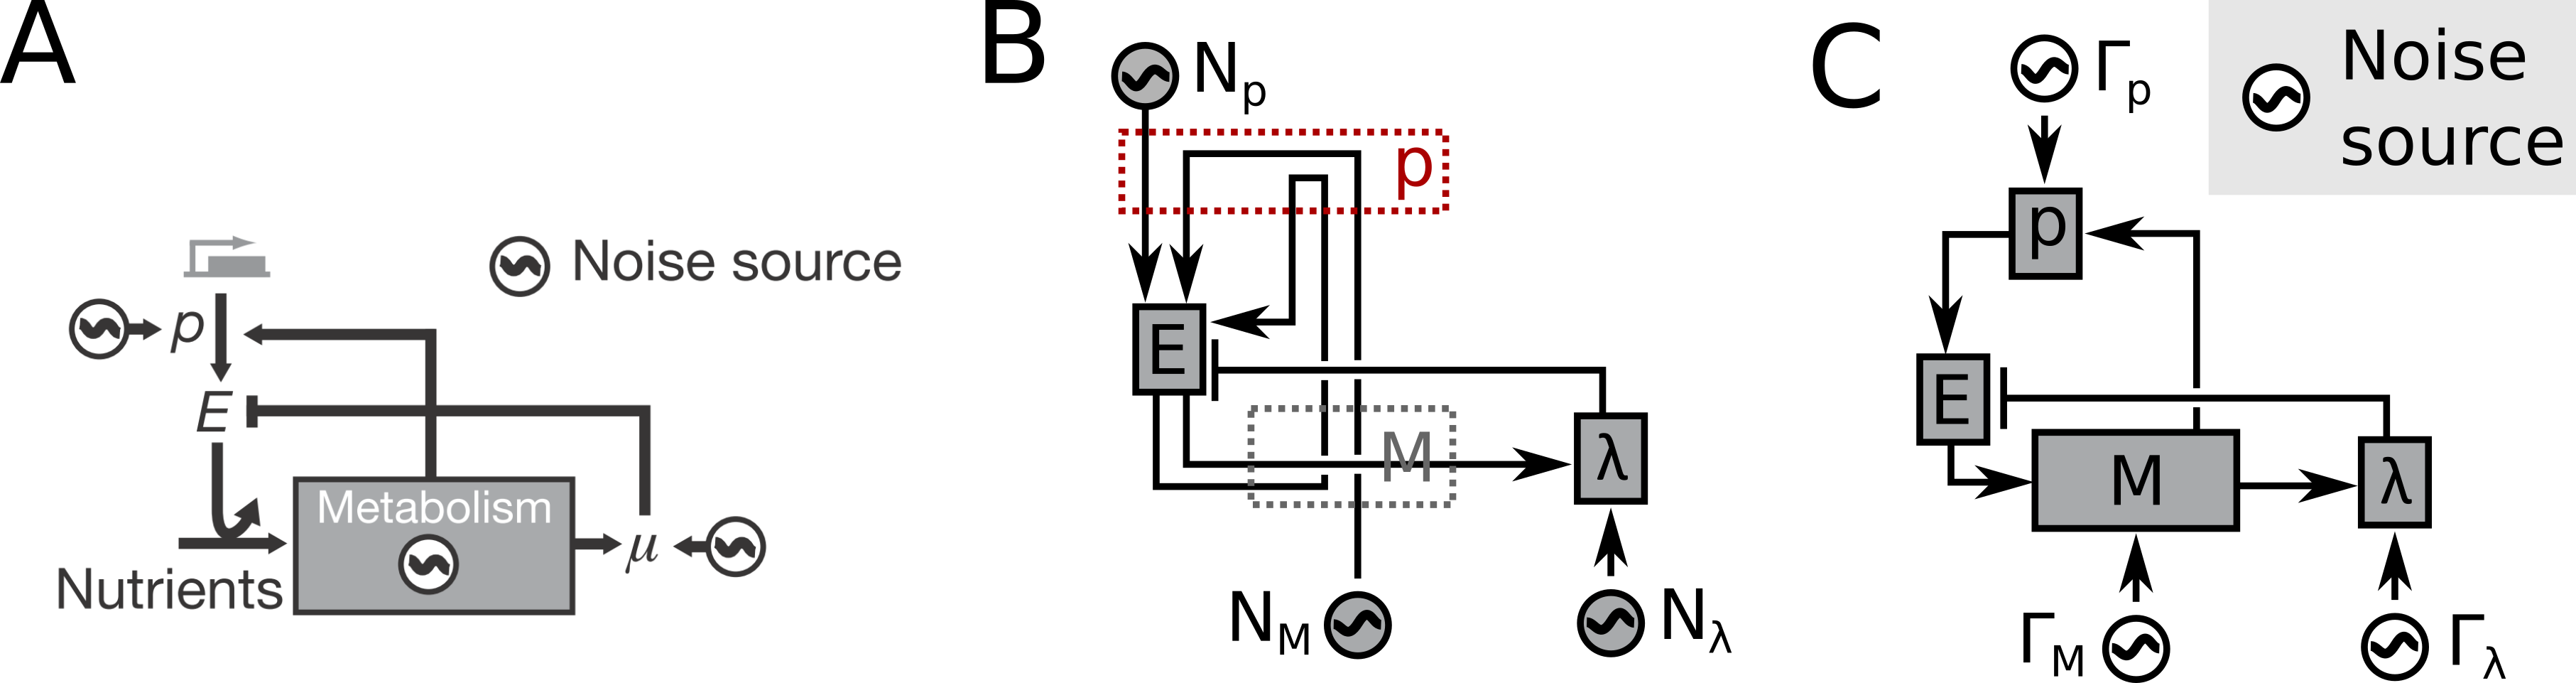
\includegraphics[width=0.9\textwidth]{model_nghe_v2.png}
	\caption{ 
		(A) Original diagram as printed in Kiviet et al. \cite{Kiviet2014}.
		(B) More technical diagram stating the relations between parameters of interest (gray boxes), and noise sources $N_P$, $N_M$, and $N_\lambda$. Arrows indicate how ODEs or functions that describe the parameters of interest are coupled. 
		Arrows that go trough the red dashed box correspond to terms that not only couple the two parameters connected by the arrow, but also make up the parameter $p$ (see also main text).
		Arrows that go through the grey box are arrows which are thought to be biologically connected to the metabolism.
		(C) An alternative version of the model with more parameters modelled explicitly. Noise sources are printed white in this diagram since they are not described by separate ODEs, which was the case in Kiviet et al. \cite{Kiviet2014}. 
	}
	\label{fig:modeldrawing}
\end{figure}

A straight forward way to model a system with these parameters, is writing down an ordinary differential equation (ODE) for each parameter involved. 
%
The Nghe model takes a somewhat different approach (it is more concise), which will be discussed later.
%
The ODEs below relate to the cartoon in Fig. \ref{fig:modeldrawing}.C
and describe the dynamics per parameter:
%
\begin{align}
\label{myfirstequation}
\dot{M} = & - \frac{(M-M_0)}{\tau}  \nonumber \\ 
          & + c_M \cdot \Gamma_M  \nonumber \\ % (1-T_{M\leftarrow E})
          & + T_{M\leftarrow E} \cdot c_M' \cdot (\frac{E}{E_0} - 1)  
\end{align}
% deltaMetabolism = -(metabolismValues(end)-parameters.metabolism0) * 1/parameters.dampingTimeMetabolism + ... % damping; 1 is the equilibrium value
% (1-parameters.transmissionEnzymeMetabolism) * ((rand()-.5)*2) * parameters.noiseSizeMetabolism + ...                              % white noise component
% parameters.transmissionEnzymeMetabolism * (enzymeValues(end)/parameters.enzymeTarget-.5) * parameters.noiseSizeMetabolism;             % noise component due enzyme
%
%
\begin{align}
	\dot{\lambda} = & -\frac{(\lambda - \lambda_0 )}{\tau_\lambda} \nonumber \\ 
 			& + c_\lambda \cdot \Gamma_\lambda \nonumber \\  %  (1-T_{\lambda\leftarrow M}) \cdot
			& + T_{\lambda\leftarrow\ M} \cdot c_\lambda' \cdot (\frac{M}{M_0}-1) 
\end{align}
%
\begin{align}
\label{mythirdequation}
\dot{P} = & - \frac{(P-P_0)}{\tau_P} \nonumber \\ 
		 & + c_p \cdot \Gamma_p \nonumber \\ 
         & + T_{P\leftarrow M} \cdot c_P' \cdot (\frac{M}{M_0}-1)  \nonumber \\ 
         & + R_{P\leftarrow M} \cdot c_P' \cdot (\frac{M}{M_0}-1)
\end{align}
%
\begin{align}
\label{mylastequation}
\dot{E} = P - \lambda E
\end{align}
%
Where $M$ describes the state of the metabolism, $\lambda$ is the growth rate, $P$ is the production rate, $E$ is the amount of enzyme, $\tau$ is a dampening term ($X_0$ is the equilibrium value), $T_{X \leftarrow Y}$ is the noise transmission constant from $X$ towards $Y$, $c_X$ and $c_X'$ are constants that set the size of the fluctuations, $\Gamma_X$ is a white noise source.
$R_{X \leftarrow Y}$ indicates a regulatory interaction, an addition to the model, but this notation is just cosmetic, as $T_\text{effective}=T+R$.
%
This model assumes all parameters have an average value from which fluctuations deviate, but always return. Hence the dampening terms.
With respect to transmission, I furthermore rescale the absolute value of the noise to be comparable to the target noise (hence the $M_0^{-1}$ and $c_X$ terms in combination with the $T_{X\leftarrow Y}$ term).

This is similar to the model that Philipe Nghe suggested in Kiviet et al. \cite{Kiviet2014}, which was inspired by Dunlop et al. \cite{Dunlop2008} (see supplement of that manuscript for a description of the Dunlop model).
%
A difference between my equations, the Nghe equations and the Dunlop equations lies in the dampening terms (those containing $\tau$, $\beta$ or $\mu_E$). In my model noise is effected through the ODE, and dampening occurs on the parameter of interest. In Dunlop et al., there are two dampening terms, one specifically dampening the noise and a second term dampening the parameters of interest. \red{Nghe also takes the latter approach, see below.}
% dampening being effected through the $(-\beta_X \cdot N_X)$ term and the $\mu_E$ parameter (see later for a more involved discussion on these parameters)}.

The correlations between these equations can be found by linearizing them, writing the correlations in Fourier space, and back-transforming them using residue integration techniques. 
\red{These notes do} not fully explores this, but \red{this will partially be discussed later}.
First, a comparison of the above model with the Nghe model is made.

\subsubsection*{Numerical implementation}

Out of practical considerations, we numerically solved Eq. \ref{myfirstequation}-\ref{mylastequation} by simple Euler propagation implemented in Matlab.
%
The script \texttt{growthnoisepropagatorv2.m} will be made available in an online Github repository, parameter settings that were used are shown below.
%
For the dilution mode: 
\begin{gather*}
E_0= 2000,
\mu_0= 1,
%\lambda_0= 0.6931,
\lambda_0= 0.0116, 
\nonumber \\ p_0= 23.1049, 
C_0= 1,
\tau_\lambda= 120,
\Gamma_\lambda= 8.3255e-04,
\Gamma_\lambda'= 8.3255e-04,
\nonumber \\ \tau_p= 120,
\Gamma_p= 0.0048,
\Gamma_p'= 0.0048,
\tau_C= 120,
\Gamma_C= 1.0000e-03,
\Gamma_C'= 1.0000e-03,
%dampingNoiseOnly= Inf,
\nonumber \\ T_{C\rightarrow\lambda}= 0,
T_{C\rightarrow{p}}= 0,
T_{E\rightarrow{C}}= 1,
T_{\lambda\rightarrow{E}}= -1;
%interactionCProduction= 0,
\end{gather*}
%
($\lambda$ is given in units of $min^{-1}$ here.)
For the catabolic mode: 
\begin{gather*}
E_0= 2000,
\mu_0= 1,
%\lambda_0= 0.6931,
\lambda_0= 0.0116,
\nonumber \\ p_0= 23.1049,
C_0= 1,
\tau_\lambda= 60,
\Gamma_\lambda= 0,
\Gamma_\lambda'= 8.3255e-06,
\nonumber \\ \tau_p= 60,
\Gamma_p= 1.5200,
\Gamma_p'= 1.5200,
\tau_C= 60,
\Gamma_C= 0,
\Gamma_C'= 0.3162,
%dampingNoiseOnly= Inf,
\nonumber \\ T_{C\rightarrow\lambda}= 0.9000,
T_{C\rightarrow{p}}= 0,
T_{E\rightarrow{C}}= 0.9000,
T_{\lambda\rightarrow{E}}= -1;
%interactionCProduction= 0,
\end{gather*}
For the common mode: 
\begin{gather*}
E_0= 2000,
\mu_0= 1,
%\lambda_0= 0.6931,
\lambda_0= 0.0116,
\nonumber \\p_0= 23.1049,
C_0= 1,
\tau_\lambda= 6,
\Gamma_\lambda= 0,
\Gamma_\lambda'= 8.3255e-06,
\nonumber \\ \tau_p= 6,
\Gamma_p= 0,
\Gamma_p'= 0.0481,
\tau_C= 60,
\Gamma_C= 0.3162,
\Gamma_C'= 0.3162,
%dampingNoiseOnly= Inf,
\nonumber \\ T_{C\rightarrow\lambda}= 0.9000,
T_{C\rightarrow{p}}= 0.9000,
T_{E\rightarrow{C}}= 0,
T_{\lambda\rightarrow{E}}= -1;
%interactionCProduction= 0,
\end{gather*}
For the combined scenario: 
\begin{gather*}
E_0= 2000,
\mu_0= 1,
%\lambda_0= 0.6931,
\lambda_0= 0.0116,
\nonumber \\p_0= 23.1049,
C_0= 1,
\tau_\lambda= 60,
\Gamma_\lambda= 2.4034e-04,
\Gamma_\lambda'= 2.4034e-04,
\nonumber \\ \tau_p= 60,
\Gamma_p= 0.5308,
\Gamma_p'= 0.5308,
\tau_C= 60,
\Gamma_C= 0.1459,
\Gamma_C'= 0.1459,
%dampingNoiseOnly= Inf,
\nonumber \\ T_{C\rightarrow\lambda}= 0.2700,
T_{C\rightarrow{p}}= 0.3000,
T_{E\rightarrow{C}}= 0.2700,
T_{\lambda\rightarrow{E}}= -1,
%interactionCProduction= -0.2700,
\end{gather*}
%
Cross-correlations were calculated based on 100000 one-minute timesteps, noise was introduced with the matlab function \texttt{normrnd}.
% 
The feedback is added by subtracting $0.27$ from the $T_{C\rightarrow\lambda}$ parameter, i.e. setting it to zero.

\subsection*{Separate noise equations}

Both Nghe and Dunlop define separate ODEs for the noise terms:
%
\begin{align}
\label{eq:generalgillespienoise}
\dot{N}_X = \sqrt{C_X} \cdot \Gamma_X - N_X/\tau
,
\end{align}
%
though their notation might be slightly different (I used Daniel Gillespie's notation \cite{Gillespie1996}; a capital C is used here to follow Gillespie's square root notation, $\sqrt{C_X}=c_x$).
With for our case $X$ equaling $\lambda$, $M$ or $P$. Note that $\tau^{-1}=\beta$ ($\beta$ is used in Nghe and Dunlop).

Not so relevant for our case, but noteworthy, is that in the Dunlop model, which models a completely different process than the one described here \cite{Dunlop2008}, the \textit{solutions} of the ODEs describing the noise are plugged into the ODEs describing the protein dynamics. This leads to an additional memory effect.
%
That is:
%
\begin{align}
\label{dunlopgeneralequation}
\dot{X} = & N_X  + F(X) + X/\tau
,
\end{align}
%
with $F(X)$ some arbitrary function of $X$. 
Note that the $N_X$ function also contains a $\tau$ term (see Eq. \ref{eq:generalgillespienoise}), which is effectively integrated, thus leading to effects of the fluctuations much longer timescales than $\tau$. 
This effect is (partially) countered by the third term in Eq. \ref{dunlopgeneralequation}, which also contains the $\tau$ term.

\subsection*{Nghe model}

As mentioned, the Nghe model takes a different approach. 
The formulae that follow correspond to Fig. \ref{fig:modeldrawing}.B (Fig. \ref{fig:modeldrawing}.A contains the version of the cartoon which was published in Kiviet et al.).
The starting point,
%
\begin{align}
\label{eq:Nghe1}
\dot{E} = P - \lambda E
,
\end{align}
%
is the same in my model, but after linearization (defined as $X=X_0+\delta X$) this leads to only one ODE:
% CONVENIENT NOTE TO SELF: %%%%%%%%%%%%%%%%%%%%%%%%%%%%%%%%%%%%%%%%%%%
% See written notes from 28.9.2016 for explicit linearization.
% END CONVENIENT NOTE TO SELF: %%%%%%%%%%%%%%%%%%%%%%%%%%%%%%%%%%%%%%%
%
\begin{align}
\label{eq:ODEElinearized}
\frac{ \delta{\dot{E}} }{E_0 \mu_0} 
+ \frac{\delta E}{E_0} 
%& = 
%\left[
% T_{E \leftarrow E} \frac{\delta E}{E_0} + T_{E \leftarrow G} N_G + N_E 
% \right]
% + T_{E \leftarrow \mu} \frac{\delta \mu}{\mu_0} \nonumber \\
& =
\frac{\delta p}{E_0 \mu_0} + T_{E \leftarrow \mu} \frac{\delta \mu}{\mu_0}
.
\end{align}
%
Noise terms are introduced with ODEs that are also shown above in Eq. \ref{eq:generalgillespienoise}.
 Additionally, two functions are defined for $p$ and $\lambda$. These are not ODEs, as the effects on these parameters are thought to happen on fast timescales. The parameters are however linearized (and thus written as $\delta X$). The equation
%
\begin{align}
\label{eq:Nghe3}
\frac{\delta\mu}{\mu_0} = T_{\mu \leftarrow E} \frac{\delta E}{E_0} + T_{\mu \leftarrow G} N_G + N_\mu
\end{align}
%
simply defines the evolution of $\delta \mu$.
There is also a similar equation for $\delta p$:
%
\begin{align}
\label{eq:Nghe4}
\frac{\delta{p}}{E_0 \mu_0} = T_{E \leftarrow E} \frac{\delta E}{E_0} + T_{E \leftarrow G} N_G + N_E
,
\end{align}
%
which plays a bit more complicated role.
It is defined using terms that pertain to E, like $T_{E \leftarrow G}$, such that it can be directly plugged into Eq. \ref{eq:ODEElinearized}. 
Indeed, plugging Eq. \ref{eq:Nghe4} into Eq. \ref{eq:ODEElinearized} leads to equation:
%
\begin{align}
\label{eq:Nghe5}
\frac{ \delta{\dot{E}} }{E_0 \mu_0} 
+ \frac{\delta E}{E_0} 
& = 
\left[
 T_{E \leftarrow E} \frac{\delta E}{E_0} + T_{E \leftarrow G} N_G + N_E 
 \right]
 + T_{E \leftarrow \mu} \frac{\delta \mu}{\mu_0} 
\end{align}
%
which corresponds to equation 5 in the Kiviet et al. \cite{Kiviet2014} manuscript.
I say it is a bit complicated, since Eq. \ref{eq:Nghe4} has no role in the model (we could also just have defined Eq. \ref{eq:Nghe5} immediately), except that it shows us which part of the model can be interpreted as being the production rate.
This is also the reason why $p$ is depicted as a red dashed box in Fig. \ref{fig:modeldrawing}.

%
%{\color{red}
%There are currently a few things unclear about Eq. \ref{eq:Nghe3} and Eq. \ref{eq:Nghe4} (respectively Eq. 3 and 4 in the Kiviet et al. manuscript):
%\begin{itemize}
%\item It seems that the transmission terms $T_{X\leftarrow Y}$ state how the parameter of interest ($X$) is affected by another parameter of interest ($Y$), however, for this to be true, the left-hand side parameter should match the first parameter in the subscript of $T$. E.g. how can a $T_{E\leftarrow G}$ term appear in the equation for $\delta p$ and moreover, what does the term $T_{E \leftarrow E}$ mean?
%\item It is not clear to me how these formulae relate to the diagram that was drawn (see Fig. \ref{fig:modeldrawing}). Why is E directly effecting $\mu$? Should there not also be a metabolism term $G$ or $\delta G$? Also why does the formula for $\delta p$ contain transmission from $E$ (assuming $T_{E\leftarrow E}$ was a type and should have been $T_{p\leftarrow E}$)? Why does the formula for $\delta p$ contain a noise term for E (ie. $N_E$)?
%\item These are not ODEs (which would seem more natural to me), probably this is intended this way, and the relationship between the parameters is defined as such. (And could be derived from ODEs.)    
%\end{itemize}
%%I am currently not sure how these equations relate to my own equations, as subscripts in Eq. \ref{eq:Nghe4} seem inconsistent with the fact that transmission should be towards $P$ (e.g. what is $T_{E\leftarrow E}$?).
%}
%
%In any case, given that noise and other parameters are related in terms of parameters (not derivatives), the following formulae are probably underlying the Nghe model:
%
%\begin{align}
%\dot{M} = & \dot{N}_M  \nonumber \\ 
%& + T_{M\leftarrow E} \cdot c_M \cdot (\frac{E}{E_0} - 1)  
%\end{align}
%
%\begin{align}
%\dot{\lambda} = & \dot{N}_\lambda \nonumber \\ 
%& +    T_{\lambda \leftarrow M} \cdot c_\lambda \cdot (\frac{M}{M_0}-1) 
%\end{align}
%
%\begin{align}
%\dot{P} = & \dot{N}_P \nonumber \\ 
%& + T_{P\leftarrow M} \cdot c_P \cdot (\frac{M}{M_0}-1)  \nonumber \\ 
%& + R_{P\leftarrow M} \cdot c_P \cdot (\frac{M}{M_0}-1)
%\end{align}
%
%Where the normalizations by $X_0$ were left out again.

Note that dampening terms can be implicitly present in the Nghe model, in the form of a transmission from the parameter to itself.
Specifically, $T_{E \leftarrow E}$ can fulfill this role. % when it is negative and $<1$. 
Second order dampening can also occur, 
as is pointed out in the Kiviet et al supplementary information, which states that the time scale of the $E$ fluctuations is set by the term $\mu_0(1-T_{E \leftarrow \mu}T_{\mu \leftarrow E}-T_{E \leftarrow E})$.

% I previously thought that dampening was not present in the Nghe model, but this is not the case.
% Here the previous text:
%Note however, that this results in the absence of dampening terms on the parameters $X$ themselves, which might lead to 
%%non-steady state behavior of the parameters.
%unstable behavior of the parameters.
%The term $X/\tau$ could be added to each of the equations to resolve this issue; the term $-N_X/\tau$ from the noise ODEs could then be dropped.
%{\color{red}Note that a $\mu_E$ term appears eventually in Nghe's equations, which might play the role of a second dampening term.}



%%%%%%%%%%%%%%







% Notes
% 
% For format of Scientific Reports, see:
% https://www.nature.com/srep/publish/guidelines#format-manuscripts
% - Title length 20 words
% - Main text 4500 words ("guide")
% - Abstract: 200 words (no refs)
% 	> "General introduction to the topic and as a brief, non-technical summary of the main results and their implications"
% - Note that figure captions cannot be more than 350 words
% - Preferably, method section limited to 1500 words
% - results may have subheadings
%
% For format of PLOS ONE, see:
% http://journals.plos.org/plosone/s/submission-guidelines
% - 2 titles, long and short: 250 characters, short title: 100 characters
% - abstract 300 words
% - ..?
% 
% Art of presenting science

% Notes on literature:
% Also check CRP page on ecocyc: https://biocyc.org/gene?orgid=ECOLI&id=CPLX0-226.


%\chapter{Negative metabolic feedback suppresses cell wide fluctuations}
\chapter{CRP responds dynamically to internal noise}
\label{chapter:CRP}

\textit{Martijn Wehrens, Laurens H.J. Krah, Benjamin D. Towbin, Rutger Hermsen, Sander J. Tans}

% Chapter clear first page
\thispagestyle{empty}
\clearpage


\section{Abstract}

\section{Introduction}

%%% ------------------------
% Let's first define the problem (or knowledge gap)
%%% ------------------------

The world is unpredictable. To survive bacteria need to respond to unforeseen situations and express the right gene at the right time. 
% Expressing the right gene at the right time is vital for bacterial survival. 
%Cells rely on biochemical networks to control gene expression.
%(Biochemical network is a general term that refers to the chemical interactions between proteins and small molecular mechanisms.)
A bacterium, like any other cell, relies on chemical interactions between proteins and small molecules to control gene expression \cite{Bray1995, Alon2006, Alon2007, Tyson2010}.
%These interactions are also referred to as "biochemical networks".
These interactions, also referred to as "biochemical networks", 
%
%Biochemical networks 
%allow cells to deal with changes that can come both from the extracellular and the intracellular environment.
allow cells to deal with 
two types of unpredictable situations.
%dynamics.
%
On one hand, the extracellular environment might change, and a different gene expression profile is required.
On the other hand,  even without environmental changes, the stochastic nature of chemical reactions can lead to fluctuations of proteins and metabolites over time within the cell \cite{Elowitz2002,Kiviet2014}.
The architecture of the biochemical network might enable the cell to deal with these fluctuations, or even use them to its advantage (see also chapter \ref{chapter:literaturereview}).
%
%Studies often focus on how the biochemical network is designed to deal with either one or the other of these two types of dynamics.
%Studies often investigate network architecture in only one of these contexts.
Studies often investigate network architecture in only an "environmental" context or only in a "stochastic fluctuation" context.
%
However, any regulatory interaction in the cell is faced with both these contexts.
%However, any regulatory interaction in the cell is faced with both an environmental and  contexts.
%
%It is unclear to what extend regulatory interactions that are known to help the cell deal with a changing environment are affected by stochastic concentration fluctuations
This might have implications for the optimal network architecture.
%
In this work, we address the open question that connects the two:
%
are regulatory interactions that are known for their role in adaptation to environmental changes also affected by concentration fluctuations in the intracellular environment due to noise?

%%% ------------------------
% Now illustrate the setting a bit more
%%% ------------------------

To investigate this question, we take a closer look at the dynamics of regulation by the cAMP receptor protein (CRP). 
%
CRP controls 378 promoters, among which 70 transcription factors \cite{Green2014, Shimada2011}.
%
It is thought that CRP controls the expression level of all catabolic genes in concert \cite{You2013}.
%
Catabolic genes convert large carbohydrate molecules into smaller metabolites, and generate energy for the cell during this process in the form of ATP \cite{Nelson2005}.
%

MULTIPLE METABOLITES CONTROL THE ACTIVITY OF ADENYLYL CYCLASE, WHICH PRODUCES CAMP
GLUCOSE (EIIA ENZYMES) {SEE REF IN TOWBIN}
ALPHA KETO-ACIDS SUCH AS A-KG AND OAA {SEE YOU2013 ACCORDING TO TOWBIN}
ECOCYC SAYS:
\cite{Hermsen2015}

One of these metabolites is alpha-ketoglutarate ($\upalpha$-KG).
%
$\upalpha$-KG promotes the conversion of ADP to ATP
%
Specifically, we focus on the role of the negative feedback in this regulatory architecture.




by the metabolite alpha-ketoglutarate ($\upalpha$-KG) on metabolic enzyme production through the cyclic adenosine monophosphate (cAMP) and CRP \footnote{Previously CRP was also called catabolite gene activator protein (CAP).}.
This negative feedback interaction is responsible for adjusting metabolic enzyme concentrations to different sugar sources in bacterial growth medium \cite{Towbin2017, Doucette2011, You2013}.

% and ask (a) whether this regulatory interaction is affected by stochastic concentration fluctuations in its input and (b) whether CRP 


\section{More content}

Some regulatory interactions are known to help the cell deal with changes in the environment, but it is unclear how these regulatory interactions respond to concentration changes due to stochastic fluctuations.
%
In this chapter, we address this open question by looking at the cAMP receptor protein (CRP), of which the 


Studies often focus on how biochemical networks either one of these dynamics


%
An example of biochemical networks responding to extracellular change is the adjustment of enzymatic concentrations to changes in extracellular sugar sources \cite{Towbin2017}.
%For example, when extracellular food source changes, enzymatic concentrations are adjusted accordingly \cite{Towbin2017}.
But even in a constant environment, the stochastic nature of chemical reactions can lead to variations in concentrations of cellular components  \cite{Elowitz2002,Kiviet2014}, 
%Intracellular changes can result from the stochastic nature of chemical reactions \cite{Elowitz2002,Kiviet2014}, 
and a myriad of examples exist of how the biochemical network is designed to both deal with and take advantage of this noise (see also chapter \ref{chapter:literaturereview}).
One example is the suppression of spontaneous fluctuations of concentrations of proteins and metabolites by negative feedback \cite{Brandman2008, Lestas2010, Bowsher2013}.
%
These two functions --- responding to intracellular on one hand and responding to extracellular changes on the other --- are usually considered separately.

In this chapter, we investigate how these two functions --- responding to intracellular on one hand and responding to extracellular changes on the other --- that are usually considered separately, are related to each other.


%


% WHAT'S THE GAP?!!!!

\section{Introduction}

% IDEA: FIRST GENERAL QUESTION, THEN LATER GO INTO DETAILS

A straightforward view of cells growing in a constant environment might be 
that of an expanding collection of individual cells that are each perfectly adapted to the environment.
%
Each cell senses the environment, 
conveys this information using intracellular signaling molecules, 
and adjusts its gene expression accordingly to 
% This adaptation occurs by biochemical networks, 
% which make sure that the cell 
express the right amount of proteins that fit the situation \cite{Bray1995, Alon2006, Alon2007, Tyson2010}.
%
This might imply that the cellular behavior solely depends on the environment of the cell.
%
However, as discussed in chapter {chapter:literaturereview}, cellular populations are very heterogeneous \cite{Kiviet2014, Hashimoto2016}.
%
Since intracellular signaling molecules are not isolated from intracellular fluctuations, 
this might also have an effect on gene regulation.
%
Indeed, it has been found that the input-output relationship between a gene's activator and its expression can be different from one cell to the next \cite{Rosenfeld2005, Keegstra2017}.

% SOME CONVENIENT ARTICLES
\cite{Brandman2008}
\cite{Rosenfeld2007}
\cite{Zambrano2015}
\cite{Howell2012}
\cite{Nevozhay2009}
\cite{Hornung2008}
\cite{Dublanche2006}
\cite{Becskei2000}
\cite{Swain2004}
\cite{Bowsher2013}
\cite{Avery2006}
\cite{Maheshri2007}
\cite{Levine2007a}
\cite{Bennett2008a}
\cite{Smits2006}
\cite{Balazsi2011}
\cite{Raj2008}
\cite{Davidson2008}
\cite{Elowitz2002}
\cite{Bruggeman2009}
\cite{Kitano2004a}


<Feedback is known to regulate stuff \cite{Goyal2010}>

Both single cell growth rates and protein concentrations can 
which can influence GRF

Maybe put Rosenfeld here?
SOMETHING THAT EXPLAINS WHY THE FOLLOWING IS RELEVANT:
assumes fixed cellular state
[Intracellular messenger molecules might (i) measure fluctuating intracellular concentrations, (ii) fluctuate themselves, 
%
When we pick two cells within a population, their individual growth rates can easily differ by a factor of two, 
as shown by single cell experiments that measured coefficients of variation (CV, standard deviation divided by the mean).
%
Both the CV of instantaneous growth rates (single cell mass doubling rate) and cellular generation time (time between divisions) has been determined to lay between $0.2$-$0.4$ \cite{Kiviet2014, Hashimoto2016}.
%
Also gene expression is known to vary for a long time \cite{Elowitz2002}, 
the CV of gene expression from any promoter lies above 0.1 \cite{Keren2015}.


This has been suggested to influence gene regulation \cite{Rosenfeld2005}.
Groups of genes fluctuate together \cite{Stewart-Ornstein2012}
Johannes' receptor stuff


Also gene expression noise is thought to ELOWITZ
and transmit KIVIET
INTRACELL. ENVIRONMENT / IMPLICATIONS FOR MESSENGERS 

>> FOR EXAMPLE, CAMP

%
This means cellular growth rates within a population can vary a factor of two from one cell to the next.

Also in this work, we find 


% >>> Note: there should not be (too much of) a contrast, because in the end we will find these two views should exist together..

Each of the individual cells tries to maintain homeostasis 


A straightforward view of cells growing in a constant environment is that of 

Cells that grow in a constant environment 
A population of cells in steady state is often though of as an exponential mass of growing cells in homeostasis.
%

% 
However, 

\section{Introduction}

%Cellular survival critically depends on cellular decision making.
%Biochemical networks allow cells to express the right genes at the right time \cite{Bray1995, Alon2006, Alon2007, Tyson2010}.

Cellular survival strongly depends on expressing the right genes at the right time.
Biochemical networks control when a gene is expressed \cite{Bray1995, Alon2006, Alon2007, Tyson2010}.
%
Often, biochemical networks are studied in the context of a changing environment.
%







In \textit{Escherichia coli}

\section{Results}

%%%%%%%%%%%%%%%%%%%%%%%%%%%%%%%%%%
\begin{figure}
	\centering
	\includegraphics[width=1.0\textwidth]{CRP-fig0.pdf}
	\caption{ 
		(A) 
	}
	\label{fig:CRP:fig0}
\end{figure}
%%%%%%%%%%%%%%%%%%%%%%%%%%%%%%%%%%


%%%%%%%%%%%%%%%%%%%%%%%%%%%%%%%%%%
\begin{figure}
	\centering
	\includegraphics[width=1.0\textwidth]{CRP-fig1_.pdf}
	\clearpage % insert a page break
	\label{fig:CRP:fig1-2}
\end{figure}	

\clearpage

\captionof{figure}{    
	\textbf{Bulk response to metabolic perturbations.}
	A.
	B.
	C.
}
%%%%%%%%%%%%%%%%%%%%%%%%%%%%%%%%%%

%%%%%%%%%%%%%%%%%%%%%%%%%%%%%%%%%%
\begin{figure}
	\centering
	\includegraphics[width=1.0\textwidth]{CRP-fig2.pdf}
	\caption{ 
		(A) 
	}
	\label{fig:CRP:fig2}
\end{figure}
%%%%%%%%%%%%%%%%%%%%%%%%%%%%%%%%%%

%%%%%%%%%%%%%%%%%%%%%%%%%%%%%%%%%%
\begin{figure}
	\centering
	\includegraphics[width=1.0\textwidth]{CRP-fig3.pdf}
	\caption{ 
		(A) 
	}
	\label{fig:CRP:fig3}
\end{figure}
%%%%%%%%%%%%%%%%%%%%%%%%%%%%%%%%%%

%%%%%%%%%%%%%%%%%%%%%%%%%%%%%%%%%%
\begin{figure}
	\centering
	\includegraphics[width=1.0\textwidth]{CRP-fig4.pdf}
	\clearpage % insert a page break
	\label{fig:CRP:fig1-2}
\end{figure}	

\clearpage

\captionof{figure}{    
	\textbf{A simple model explains how feedback filters out noise transmission.}
	A simple model predicts correlation inversion.
	A.
	B.
	C.
}

%%%%%%%%%%%%%%%%%%%%%%%%%%%%%%%%%%

\section{Discussion}

\textbf{Talking points.} Evolution doesn't separate dynamic and steady state functionality, and can potentially optimize both.


For example, how cellular composition changes in response to different food sources has been a topic of study for a long time \cite{Schaechter1958}.
%
Regulation of metabolism has recently been shown to fit into a larger picture, in which the cell co-regulates large groups of genes together.
Each of these groups (also called sectors), relate to a major 
%
% Recently, it has been shown that large groups of genes are co-regulated, these groups are also called sectors, each of which relate to a major category of cellular activity such as 
category of cellular activity such as 
metabolism, anabolism, protein synthesis, replication, etc 
%catabolism, metabolism, anabolism, , protein synthesis, replication, etc. 
\cite{Klumpp2009, You2013, Scott2014, Hui2015, Hermsen2015, Erickson2017}.
%
% Note that Erickson is not really growth laws itself, but more about how a switch between two environments occurs
%
An important player in regulating the size of the metabolic sector is the cAMP receptor protein (CRP) \cite{Keseler2017, Grainger2005, Robinson1998, Zheng2004, Gorke2008, Fic2009, Green2014}.
%
CRP is activated by cyclic adenosine monophosphate (cAMP) and it controls 378 promoters, among which 70 transcription factors \cite{Green2014, Shimada2011}.
%
The CRP.cAMP regulation 
%
Recently, it has been shown that the CRP.cAMP regulation 

%So-called growth laws describe how the ratio between these sectors is controlled by the cells to adapt to different environments.
%
%For some sectors, it is known that their expression level can be controlled by a single molecule or protein.
%For example, guanosine tetraphosphate (ppGpp) controls ribosomal expression \cite{Cashel1969, Potrykus2008, Ross2013, Hui2015}, and the 
%cAMP receptor protein (CRP) controls expression of metabolic enzymes.
% 



\section{Methods}

% For promoter sequences, see: M_2016_06_26_CRP_s70_promoter_sequences.docx

\section*{Acknowledgements}

I thank Pieter Rein ten Wolde and Harmen Wierenga for useful discussions.

%\section{Author contributions}

\section*{Things to keep in mind}

See notes sent to me by Pieter Rein!

***

\cite{You2013}
You, C., Okano, H., Hui, S., Zhang, Z., Kim, M., Gunderson, C.W., Wang, Y.-P., Lenz, P., Yan, D., and Hwa, T. (2013). Coordination of bacterial proteome with metabolism by cyclic AMP signalling. Nature 500, 301–6. Available at: http://www.ncbi.nlm.nih.gov/pubmed/23925119 [Accessed January 20, 2014].
(This is simply the Hwa article re. proteome partitioning, but should check because they also talk about cAMP)
According to chubukov2014 this is also article that shows akg feedback to CRP.

**

\cite{Somavanshi2016}
Somavanshi, R., Ghosh, B., and Sourjik, V. (2016). Sugar Influx Sensing by the Phosphotransferase System of Escherichia coli. 1–19.

Also check out other papers in (physical) yellow folder in cabinet labeled CRP.

**

\cite{Flamholz2013}
Flamholz, A., Noor, E., Bar-Even, A., Liebermeister, W., and Milo, R. (2013). Glycolytic strategy as a tradeoff between energy yield and protein cost. Proc. Natl. Acad. Sci. 110, 10039–10044.

Fig. S2 is already worth it because it gives nice overview between how glycolysis convert glucose to pyruvate and then either ferments it or aerobically burns it to CO2 (+acetate).

**

\cite{chubukov2014} has a few nice graphs about different "activities" that need to happen in the cell (ie. categories of metabolites and how they are produced.) Also explains how CRP is controlled! Point to YOu2013 for a-kg inhibition feedback loop.

**

Stewart-Ornstein 2017 \cite{Stewart-Ornstein2017} was sent by Sander, mentions CRP, so quickly check whether might be interesting.

**

Perhaps it is interesting to check out the network topology validation by Michael Stumpf (see Heidelberg Quant conference 2017). 

**


Check also:
\cite{VanHeerden2017}
and
\cite{Nordholt2017}.

%%%%%%%%%%%%%%%%%%%%%%%%%%%%%%%%%%%%%%%%%%%%%%%%%%%%%%%%%%%%%%%%%%%%%%%%%%%%%%%%%%%%%%%%%%%%%%%%%%%%%%%%%%%%%%%%%%%%%%%%%%%%%%%%%%%%%%%%%%%%%%%%%%%%%%%%%%%%%%%%%%%%%%%%%%%%%%%%%%%%%%%%%%%%%%%%%%%%%%%%%%%%%%%%%
%%%%%%%%%%%%%%%%%%%%%%%%%%%%%%%%%%%%%%%%%%%%%%%%%%%%%%%%%%%%%%%%%%%%%%%%%%%%%%%%%%%%%%%%%%%%%%%%%%%%%%%%%%%%%%%%%%%%%%%%%%%%%%%%%%%%%%%%%%%%%%%%%%%%%%%%%%%%%%%%%%%%%%%%%%%%%%%%%%%%%%%%%%%%%%%%%%%%%%%%%%%%%%%%%

\section*{Supplementary figures}

%%%%%%%%%%%%%%%%%%%%%%%%%%%%%%%%%%%%%%%%%%%%%%%%%%%%%%%%%%%%%%%%%%%%%%%%%%%%%%%%%%%%%%%%%%%%%%%%%%%%%%%%%%%%%%%%%%%%%%%%%%%%%%%%%%%%%%%%%%%%%%%%%%%%%%%%%%%%%%%%%%%%%%%%%%%%%%%%%%%%%%%%%%%%%%%%%%%%%%%%%%%%%%%%%
%% Pulsing dynamics

\begin{figure}%%%%%%%%%%%%%%%%%%%%%%%%%%%%%%%%%%
	\centering
	\includegraphics[width=1.0\textwidth]{pdf_averagetimetraces_4.pdf}
	\includegraphics[width=1.0\textwidth]{pdf_averagetimetraces_2.pdf}
	\includegraphics[width=1.0\textwidth]{pdf_averagetimetraces_5.pdf}
	\clearpage % insert a page break
	\label{fig:XXX:XXX}
\end{figure}	

\clearpage

\captionof{figure}{    
	\textbf{blabla}
}%%%%%%%%%%%%%%%%%%%%%%%%%%%%%%%%%%%%%%%%%%%%%%%

% pdf_scattersoftraces_1

\begin{figure}%%%%%%%%%%%%%%%%%%%%%%%%%%%%%%%%%%%%%%%%%%%%%%%
	\centering
	\includegraphics[width=0.49\textwidth]{pdf_scattersoftraces_1.pdf}
	\includegraphics[width=0.49\textwidth]{pdf_scattersoftraces_2.pdf}	
	\caption{ 
		(A) 
	}
	\label{fig:CRP:XXX}
\end{figure}%%%%%%%%%%%%%%%%%%%%%%%%%%%%%%%%%%%%%%%%%%%%%%%

\begin{figure}%%%%%%%%%%%%%%%%%%%%%%%%%%%%%%%%%%
	\centering
	\includegraphics[width=1.0\textwidth]{pdf_timetracesinglecell13.pdf}
	\includegraphics[width=1.0\textwidth]{pdf_timetracesinglecell49.pdf}
	\includegraphics[width=1.0\textwidth]{pdf_timetracesinglecell144.pdf}
	\clearpage % insert a page break
	\label{fig:XXX:XXX}
\end{figure}	

\clearpage

\captionof{figure}{    
	\textbf{blabla}
}%%%%%%%%%%%%%%%%%%%%%%%%%%%%%%%%%%%%%%%%%%%%%%%



% Dynamic behavior against itself.
\begin{figure}%%%%%%%%%%%%%%%%%%%%%%%%%%%%%%%%%%%%%%%%%%%%%%%
	\centering
	\includegraphics[width=1.00\textwidth]{pdf_highlowplots_case1.pdf}
	\caption{ 
		(A) 
	}
	\label{fig:CRP:XXX}
\end{figure}%%%%%%%%%%%%%%%%%%%%%%%%%%%%%%%%%%%%%%%%%%%%%%%
\begin{figure}%%%%%%%%%%%%%%%%%%%%%%%%%%%%%%%%%%%%%%%%%%%%%%%
	\centering
	\includegraphics[width=1.00\textwidth]{pdf_highlowplots_case2.pdf}
	\caption{ 
		(A) 
	}
	\label{fig:CRP:XXX}
\end{figure}%%%%%%%%%%%%%%%%%%%%%%%%%%%%%%%%%%%%%%%%%%%%%%%
\begin{figure}%%%%%%%%%%%%%%%%%%%%%%%%%%%%%%%%%%%%%%%%%%%%%%%
	\centering
	\includegraphics[width=1.00\textwidth]{pdf_highlowplots_case3.pdf}
	\caption{ 
		(A) 
	}
	\label{fig:CRP:XXX}
\end{figure}%%%%%%%%%%%%%%%%%%%%%%%%%%%%%%%%%%%%%%%%%%%%%%%
\begin{figure}%%%%%%%%%%%%%%%%%%%%%%%%%%%%%%%%%%%%%%%%%%%%%%%
	\centering
	\includegraphics[width=1.00\textwidth]{pdf_highlowplots_case4.pdf}
	\caption{ 
		(A) 
	}
	\label{fig:CRP:XXX}
\end{figure}%%%%%%%%%%%%%%%%%%%%%%%%%%%%%%%%%%%%%%%%%%%%%%%
\begin{figure}%%%%%%%%%%%%%%%%%%%%%%%%%%%%%%%%%%%%%%%%%%%%%%%
	\centering
	\includegraphics[width=1.00\textwidth]{pdf_highlowplots_case5.pdf}
	\caption{ 
		(A) 
	}
	\label{fig:CRP:XXX}
\end{figure}%%%%%%%%%%%%%%%%%%%%%%%%%%%%%%%%%%%%%%%%%%%%%%%
\begin{figure}%%%%%%%%%%%%%%%%%%%%%%%%%%%%%%%%%%%%%%%%%%%%%%%
	\centering
	\includegraphics[width=1.00\textwidth]{pdf_highlowplots_case6.pdf}
	\caption{ 
		(A) 
	}
	\label{fig:CRP:XXX}
\end{figure}%%%%%%%%%%%%%%%%%%%%%%%%%%%%%%%%%%%%%%%%%%%%%%%





%%%%%%%%%%%%%%%%%%%%%%%%%%%%%%%%%%%%%%%%%%%%%%%%%%%%%%%%%%%%%%%%%%%%%%%%%%%%%%%%%%%%%%%%%%%%%%%%%%%%%%%%%%%%%%%%%%%%%%%%%%%%%%%%%%%%%%%%%%%%%%%%%%%%%%%%%%%%%%%%%%%%%%%%%%%%%%%%%%%%%%%%%%%%%%%%%%%%%%%%%%%%%%%%%
%Sup belonging to figure 2 %%%%%%%%%%%%%%%%%%%%%%%%%%%%%%%%%%%%%%%%%%%%%%%%%%%%%%%%%%%%%%%%%%%%%%%%%%%%%%%%%%%%%%%%%%%%%%%%%%%%%%%%%%%%%%%%%%%%%%%%%%%%%%%%%%%%%%%%%%%%%%%%%%%%%%%%%%%%%%%%%%%%%%%%%%%%%%%%%%%%%%%%%%%%%%%%%%%%%%%%%%%%%%%%%

%%%%%%%%%%%%%%%%%%%%%%%%%%%%%%%%%%
\begin{figure}
	\centering
	\includegraphics[width=1.0\textwidth]{CRP-fig2sup.pdf}
	\caption{ 
		(A) 
	}
	\label{fig:CRP:fig2}
\end{figure}
%%%%%%%%%%%%%%%%%%%%%%%%%%%%%%%%%%

%%%%%%%%%%%%%%%%%%%%%%%%%%%%%%%%%%
\begin{figure}
	\centering
	\includegraphics[width=1.0\textwidth]{pdf_chromo1prime_overview_custom_scatter_rateVsRateYC.pdf}
	\includegraphics[width=1.0\textwidth]{pdf_chromo1prime_overview_custom_scatter_concentrationVsConcentrationYC.pdf}
	\caption{ 
		(A) 
	}
	\label{fig:CRP:fig3}
\end{figure}
%%%%%%%%%%%%%%%%%%%%%%%%%%%%%%%%%%

%%%%%%%%%%%%%%%%%%%%%%%%%%%%%%%%%%%%%%%%%%%%%%%%%%%%%%%%%%%%%%%%%%%%%%%%%%%%%%%%%%%%%%%%%%%%%%%%%%%%%%%%%%%%%%%%%%%%%%%%%%%%%%%%%%%%%%%%%%%%%%%%%%%%%%%%%%%%%%%%%%%%%%%%%%%%%%%%%%%%%%%%%%%%%%%%%%%%%%%%%%%%%%%%%
%Sup belonging to figure 3 %%%%%%%%%%%%%%%%%%%%%%%%%%%%%%%%%%%%%%%%%%%%%%%%%%%%%%%%%%%%%%%%%%%%%%%%%%%%%%%%%%%%%%%%%%%%%%%%%%%%%%%%%%%%%%%%%%%%%%%%%%%%%%%%%%%%%%%%%%%%%%%%%%%%%%%%%%%%%%%%%%%%%%%%%%%%%%%%%%%%%%%%%%%%%%%%%%%%%%%%%%%%%%%%%

%%%%%%%%%%%%%%%%%%%%%%%%%%%%%%%%%%
\begin{figure}
	\centering
	\includegraphics[width=1.0\textwidth]{CRP-fig3sup.pdf}
	\caption{ 
		(A) 
	}
	\label{fig:CRP:fig3}
\end{figure}
%%%%%%%%%%%%%%%%%%%%%%%%%%%%%%%%%%

%%%%%%%%%%%%%%%%%%%%%%%%%%%%%%%%%%%%%%%%%%%%%%%%%%%%%%%%%%%%%%%%%%%%%%%%%%%%%%%%%%%%%%%%%%%%%%%%%%%%%%%%%%%%%%%%%%%%%%%%%%%%%%%%%%%%%%%%%%%%%%%%%%%%%%%%%%%%%%%%%%%%%%%%%%%%%%%%%%%%%%%%%%%%%%%%%%%%%%%%%%%%%%%%%
%Sup belonging to figure 4 %%%%%%%%%%%%%%%%%%%%%%%%%%%%%%%%%%%%%%%%%%%%%%%%%%%%%%%%%%%%%%%%%%%%%%%%%%%%%%%%%%%%%%%%%%%%%%%%%%%%%%%%%%%%%%%%%%%%%%%%%%%%%%%%%%%%%%%%%%%%%%%%%%%%%%%%%%%%%%%%%%%%%%%%%%%%%%%%%%%%%%%%%%%%%%%%%%%%%%%%%%%%%%%%%

%%%%%%%%%%%%%%%%%%%%%%%%%%%%%%%%%%%%%%%%%%%%%%%%%%%%%%%%%%%%%%%%%%%%%%%%%%%%%%%%%%%%%%%%%%%%%%%%%%%%%%%%%%%%%%%%%%%%%%%%%%%%%%%%%%%%%%%%%%%%%%%%%%%%%%%%%%%%%%%%%%%%%%%%%%%%%%%%%%%%%%%%%%%%%%%%%%%%%%%%%%%%%%%%%
%Extra sup not belonging but anyways shown %%%%%%%%%%%%%%%%%%%%%%%%%%%%%%%%%%%%%%%%%%%%%%%%%%%%%%%%%%%%%%%%%%%%%%%%%%%%%%%%%%%%%%%%%%%%%%%%%%%%%%%%%%%%%%%%%%%%%%%%%%%%%%%%%%%%%%%%%%%%%%%%%%%%%%%%%%%%%%%%%%%%%%%%%%%%%%%%%%%%%%%%%%%%%%%%%%%%%%%%%%%%%%%%%


%%%%%%%%%%%%%%%%%%%%%%%%%%%%%%
% Figure with floating caption

\begin{figure}
	\centering
	\includegraphics[width=1.0\textwidth]{pdf_chromo1_overview_means.pdf}
	\clearpage % insert a page break
	\label{fig:XXX:XXX}
\end{figure}	

\clearpage

\captionof{figure}{    
	\textbf{blabla}
}
%%%%%%%%%%%%%%%%%%%%%%%%%%%%%%

%%%%%%%%%%%%%%%%%%%%%%%%%%%%%% CRP CCs 1
% Figure with floating caption

\begin{figure}
	\centering
	\includegraphics[width=1.0\textwidth]{pdf_chromo1_CCs_Y6_mean_cycCor_muP9_fitNew_cycCor}
	\clearpage % insert a page break
	\label{fig:XXX:XXX}
\end{figure}	

\clearpage

\captionof{figure}{    
	\textbf{blabla}
}
%%%%%%%%%%%%%%%%%%%%%%%%%%%%%%

%%%%%%%%%%%%%%%%%%%%%%%%%%%%%% 2
% Figure with floating caption

\begin{figure}
	\centering
	\includegraphics[width=1.0\textwidth]{pdf_chromo1_CCs_dY5_cycCor_muP9_fitNew_atdY5_cycCor}
	\clearpage % insert a page break
	\label{fig:XXX:XXX}
\end{figure}	

\clearpage

\captionof{figure}{    
	\textbf{blabla}
}
%%%%%%%%%%%%%%%%%%%%%%%%%%%%%%

%%%%%%%%%%%%%%%%%%%%%%%%%%%%%% Consti CCs 1
% Figure with floating caption

\begin{figure}
	\centering
	\includegraphics[width=1.0\textwidth]{pdf_chromo1_CCs_C6_mean_cycCor_muP9_fitNew_cycCor}
	\clearpage % insert a page break
	\label{fig:XXX:XXX}
\end{figure}	

\clearpage

\captionof{figure}{    
	\textbf{blabla}
}
%%%%%%%%%%%%%%%%%%%%%%%%%%%%%%

%%%%%%%%%%%%%%%%%%%%%%%%%%%%%% 2
% Figure with floating caption

\begin{figure}
	\centering
	\includegraphics[width=1.0\textwidth]{pdf_chromo1_CCs_dC5_cycCor_muP9_fitNew_atdC5_cycCor}
	\clearpage % insert a page break
	\label{fig:XXX:XXX}
\end{figure}	

\clearpage

\captionof{figure}{    
	\textbf{blabla}
}
%%%%%%%%%%%%%%%%%%%%%%%%%%%%%%

%%%%%%%%%%%%%%%%%%%%%%%%%%%%%% Branches mu
% Figure with floating caption

\begin{figure}
	\centering
	\includegraphics[width=1.0\textwidth]{pdf_chromo1_branches_muP9_fitNew_cycCor}
	\clearpage % insert a page break
	\label{fig:XXX:XXX}
\end{figure}	

\clearpage

\captionof{figure}{    
	\textbf{blabla}
}
%%%%%%%%%%%%%%%%%%%%%%%%%%%%%%

%%%%%%%%%%%%%%%%%%%%%%%%%%%%%% Branches Y (CRP)
% Figure with floating caption

\begin{figure}
	\centering
	\includegraphics[width=1.0\textwidth]{pdf_chromo1_branches_Y6_mean_cycCor}
	\clearpage % insert a page break
	\label{fig:XXX:XXX}
\end{figure}	

\clearpage

\captionof{figure}{    
	\textbf{blabla}
}
%%%%%%%%%%%%%%%%%%%%%%%%%%%%%%

%%%%%%%%%%%%%%%%%%%%%%%%%%%%%% Branches dY (CRP)
% Figure with floating caption

\begin{figure}
	\centering
	\includegraphics[width=1.0\textwidth]{pdf_chromo1_branches_dY5_cycCor}
	\clearpage % insert a page break
	\label{fig:XXX:XXX}
\end{figure}	

\clearpage

\captionof{figure}{    
	\textbf{blabla}
}
%%%%%%%%%%%%%%%%%%%%%%%%%%%%%%





%%%%%%%%%%%%%%%%%%%%%%%%%%%%%%%%%%
\begin{figure}
	\centering
	\includegraphics[width=1.0\textwidth]{pdf_plasmids2_overview_correlations_CmuPmu_G.pdf}
	\caption{ 
		\textbf{Without feedback, metabolic fluctuations transmit to growth.}
		The interaction of metabolic and growth fluctuations was measured by plasmid constructs.
		(A) 
	}
	\label{fig:CRP:plasmidCCs}
\end{figure}
%%%%%%%%%%%%%%%%%%%%%%%%%%%%%%%%%%








%\chapter{The Ribosomal City}
%\chapter{The Ribosome, a puzzling protein-rna complex}
\chapter{Ribosomal dynamics, a puzzling affair}
\label{chapter:ribosomes}


%%%%%%%%%%%%%%%%%%%%%%%%%%%%%%%%%%%%%%%%%%%%%%%%%%%%%%%%%%%%%%%%%%%%%%%%%%%%%%%%%%%%%%%%%%%%%%%%%%%%%%%%%%%%%%%%%%%%%%%%%%%%%%%%%%%%%%%%%%%%%%%%
% Picture of the ribosome
%%%%%%%%%%%%%%%%%%%%%%%%%%%%%%%%%%%%%%%%%%%%%%%%%%%%%%%%%%%%%%%%%%%%%%%%%%%%%%%%%%%%%%%%%%%%%%%%%%%%%%%%%%%%%%%%%%%%%%%%%%%%%%%%%%%%%%%%%%%%%%%%

\begin{figure}
    \centering    
    %\includegraphics[width=1.0\textwidth]{pdf_2016-02-17_pos2_L31-mCerulean_clouds.pdf}
    \includegraphics[width=0.8\textwidth]{ribosomes_allproteinscolored.png}
    \caption{ 
        \textbf{Picture of the ribosome.}
        The ribosome consist of a small and a large subunit. These two come together on messenger RNA templates to perform protein synthesis.
        The complete ribosome is made of 3 ribosomal RNA molecules and more than 50 proteins, shown in grey and color in the picture above, respectively \cite{Chen2013}.
        The 16S rRNA and 23S rRNA molecules function as backbone. % for the small and large subunits, respectively.
        Proteins labeled S1 up to S22 
        % (S22 being sub-stoichiometric) 
        bind to the 16S rRNA to form the small subunit, and proteins labeled L1-L36 and the 5S rRNA bind to the 23S rRNA to form the large subunit \cite{Keseler2017}.
        The Ecocyc database lists 58 ribsomal proteins, though also different numbers of ribosomal proteins are listed (ref. \cite{Chen2013} e.g. talks about 54 ribosomal proteins).
        % The 5S rRNA also binds to the large subunit.
        Interestingly, the ribosomal RNA constitutes 73-80\% of the total RNA found in an \textit{E. coli} cell (mRNA constitutes 3-4.5\% and tRNA 15-20\%) \cite{Norris1972}.
        Assembly of the ribosome also requires many co-factors \cite{Chen2013}. % note also DnaK is required.
        %
        This image is based on x-ray crystallography (PDB ID: 4v4q, \cite{Schuwirth2005}). Pdb files downloaded from \texttt{www.rcsb.org} \cite{Berman2000} 
        visualized with UCSF Chimera (version 1.11.2, build 41376, \cite{pettersen2004}).
        % Previously, I seemed to have used 4v4a, which is from 2003 http://www.rcsb.org/pdb/explore.do?structureId=4v4a.        
        %
        %        
    }
    \label{fig:ribo:pictureofribo}
\end{figure}

%%%%%%%%%%%%%%%%%%%%%%%%%%%%%%%%%%%%%%%%%%%%%%%%%%%%%%%%%%%%%%%%%%%%%%%%%%%%%%%%%%%%%%%%%%%%%%%%%%%%%%%%%%%%%%%%%%%%%%%%%%%%%%%%%%%%%%%%%%%%%%%%

\section{Introduction}

\subsection{The central role of the ribosome}

Ribosomes are life.
%
In 1958, Francis Crick, who discovered the structure of DNA with James Watson and Rosalind Franklin,
formulated what is called the central dogma of molecular biology.
This states 
% declares 
that DNA holds the amino acid sequence information required to build a protein, and that this sequence information is first translated to RNA, which is then transcribed into a protein \cite{Crick1958}.
% 
This dogma relates immediately to some of the features that are said to define life: 
the capability to store information and 
the regeneration of components from scratch \cite{Lawrence2005, Koshland2002}.
%
Also around that time, 
Slightly earlier, in 1955, "new cytoplasmic components" were already discovered under an electron microscope \cite{Palade1955}.
These components turned out to be the components in the cell that perform the last step of the central dogma: 
the synthesis of proteins using mRNA molecules as templates; also known as transcription.
The components became known as ribosomes.
%
% Given the central place of the ribosome, in the circle of life, and 
Given the idea that early life consisted only of RNA molecules that could catalyze other reactions (the "RNA world" \cite{Campbell2002}), it is not surprising that the ribosomes 
% these components of the cell
consist of both catalytic RNA and proteins,
as shown in figure \ref{fig:ribo:pictureofribo}.
%
%As such, it is not only an embodiment of the central dogma, but also the exception to the rule.
As such, we can say ribosomes are a key element of life.

% life
% Lawrence: information storage, catalysts, energy relation environment, grow and reproduce, respond stimuli
% Koshland: program, improvisation (MW: long term adaptation), compartmentalization, energy, regeneration, adaptabilty (short term adaptation), seclusion (being able to separate different processes, e.g. enzyme's specifity).

\subsection{Understanding the role of ribosomes in protein fluctuations}

In this thesis, 
we have been trying to further 
% When we want to understand the cell, ribosomes are a good starting point.
%It is our aim to better 
understand % cellular dynamics.
temporal fluctuations in the concentrations of cellular components.%, which occur due to the intrinsic stochastic nature of chemical processes that underlay cellular 
%
As mentioned in earlier chapters (\ref{chapter:literaturereview} and  \ref{chapter:CRP}),
these fluctuations are a result of the intrinsic stochastic nature of chemical processes that occur in the cell.
% (see also previous chapters \ref{chapter:literaturereview} and  \ref{chapter:CRP}).
%
Given the central role of the ribosome in the cell that was just discussed, ribosomes might play a big role in such fluctuations.
%Since ribosomes are key components in the cell, 
Indeed, it is often suggested that fluctuations in ribosomal concentration could result in cell-wide protein concentration fluctuations \cite{Davidson2008, Raj2008, Chalancon2012, Bruggeman2018}.
%
Such concerted concentration fluctuations are also referred to as extrinsic noise (as opposed to intrinsic noise, fluctuations that only occur in one cellular species) \cite{Elowitz2002}.

\subsection{Quantifying ribosomal dynamics}
\label{section:ribos:walker}

In a previous thesis from the Tans lab, Noreen Walker 
% In previous work from our lab, Walker et al. 
quantified the dynamic relationship between single cell ribosomal expression fluctuations and growth in steady state conditions \cite{Walker2016t}.
%
The experiments involved presented many challenges, 
of which a number is described in her thesis.
%
% The results from these experiments were rather inconclusive.
%
Given previously described central role of the ribosome, 
it was hypothesized that the stochastically fluctuating concentration of ribosomes might be limiting, 
meaning that ribosomal fluctuations might result in growth rate fluctuations.
%
In single cell time lapse experiments, no clear indications were found to support this hypothesis.
%
Instead, 
ribosomal proteins L19 and L31 that were labeled with mCherry (L31-R and L19-R)
% mCherry-labeled L31 and L19 subunits (L31-R and L19-R) 
showed expression-growth cross-correlations (CCs) indicative of dilution-scenario behaviour in minimal medium, or none at all in rich medium (see chapters \ref{chapter:literaturereview} and \ref{chapter:CRP} for discussions about the use of cross-correlations to interpret dynamics). 
mCerulean labeled L31 ribosomal protein (L31-C) showed expression-growth CCs with small correlations around zero delay 
% at positive delays 
%between expression and growth 
in minimal medium.
This difference between the L31-C and L31-R experiments was unexpected, as only the label was different.
%
In rich medium, the L31-C cross-correlation was consistent with the L31-R cross-correlation, and showed almost no correlation.
%
Since the ribosome mainly consists of RNA, 
a GFP reporter under the control of one of the ribosomal RNA promoters was also used (rrna-G).
Like the L31-C reporter, the dynamics of this rrna-G reporter showed positive correlations in minimal medium and only very small correlations in rich medium.
% an additional reporter was used which consisted of the ribosomal RNA promoter 
%
Also growth-expression scatter plots were used, to investigate possible interesting shapes of growth-expression relationships, but this yielded no noteworthy shapes.

In an attempt to force the cell in a scenario where ribosomes are limiting, experiments were conducted where cells were grown in the presence of sub-inhibitory concentrations of tetracycline, an antibiotic.
%
Though also interesting in itself, the outcome of such an experiment could serve as a reference to interpret other experiments.
%
In rich medium, both for the L31-R and the rrn-G reporter, the antibiotic did not result in more limiting behaviour, i.e. correlations did not become more positive.
%
Given the disparate observations, both between reporters and conditions, 
and the absence of a point of reference,
the nature of the ribosomal dynamics remained fairly elusive; it was concluded that ribosomal fluctuations perhaps do not have a pivotal role in steady state cellular growth dynamics.

\subsection{New work}

In this chapter, we will describe a few additional experiments that were aimed at gaining further insights in the ribosomal dynamics.
Specifically, we tried to understand whether fluctuations in ribosomal concentration could have cell-wide implications.
%
To answer this question, we tried both new experiments as well increase the throughput of existing experiments.
%
Since this is an ongoing project, this chapter will be more succinct than previous ones.

\section{Results}
% > looked at dual reporters with pn25 reporter to assess effect from ribosomal concentration > protein production
    % ^> (outlook) Note that also R_CR-pq would be interesting in future with minor technical adjustment
% > looked at shift experiment to look at a (dynamic) environment where we knew cells with more ribosomes have an advantage
% > Additional semi-steady state measurements w/ and w/o antibiotics (incl. the pn25 reporter)
% > (outlook) we also looked into adding a plasmid that would introduce a burden unto the ribosomes 
%	% ^> Note that cells will adjust, so in a sense this might not increase the effect of fluctuations (perhaps put in sketch of two graphs with two optimums)
% > (outlook) we also looked into rrna reporter in delta(rna) strains
% > (outlook) maybe r-proteins are not as stochastically equivalent as sometimes assumed, ratio Y_m9:Y_ab and R_m9:R_ab not equal (2.4 and 2.3)
    % ^> what about production though, that's ratio_Y 3.18 vs. 2.15, should these ratios not be equal? --> not to C-ratio as the growth rates differ.
% > (outlook) ppgpp titration
% > (outlook) perhpas the fluctuations in total ribosome activity are a difficult function of fluctuations in all of the separate ribosomal components, which all might have their own (partially) independent contributions, and therefor it is hard to see single correlations. (the C

\subsection{Additional strains}

\begin{table}[h]
    \begin{tabularx}{\textwidth}{llXl}
        %
        \textbf{ASC number}	& \textbf{Shorthand} & \textbf{Description} & \textbf{Source}		\\
        \hline
        ASC976  &	Prrna-C, pn25-Y	&	Δphp::pn25-mVenus-cmR, Δche::Prrsa-mCerulean-kanR. (Kanamycin and chloramphenicol resistance.)  & VS \\
        %     
        ASC968	& L19-C, pn25-Y	& L19-gc-mCerulean-kanR (GC linker), Δ(…)::pn25-mVenus-cmR.	(Kanamycin and chloramphenicol resistance.)	& VS \\
        %
        ASC1058	& L9-R, S2-Y	& Also known as JE202. rplI-mCherry-KanR (L9), rpsB-venus-CmR (S2). (Kanamycin and chloramphenicol resistance.) Gift from Johan Elf lab. & \cite{Wallden2016} \\
        \hline
        %
        % ASC631 & pn25-R, lacA-G & $\Delta$lacA::gfp-cat, $\Delta$php::pn25-mCherry-kanR & \cite{Kiviet2014} \\
        ASC666 & L31-R, gltA-G  & L31::mCherry-kanR, gltA::gfpA206K-cat & \cite{Kiviet2014} \\
        ASC810	& L31-C & L31-gc-mCerulean-kanR (GC linker). (Kanamycin resistant.) & NW, VS \\
        \hline
    \end{tabularx}
    \caption{\textbf{Strains used in this chapter.} Strain ASC1058 was a kind gift from the Johan Elf lab. VS indicates these strains were created by Vanda Sunderlikova, technician in the Tans lab. ASC stands for AMOLF strain collection. Note that Y, C, G and R indicate yellow, cyan, green and red fluorescent reporters, respectively. The first two strains in this table were specifically created for experiments described in this chapter, and the third strain was requested specifically for work described in this chapter. The last two strains in the table were created earlier.}
    \label{table:ribostrains1}
\end{table}

%To be able to further explore the interaction of ribosomal expression with cellular dynamics, 
To be able to further explore the implications of ribosomal fluctuations, 
we produced additional strains.
%
Importantly, we were interested in the effect fluctuations in ribosomal expression would have on 
the single cell capacity to produce proteins.
%single cell protein production.
%
We therefore created two dual-label strains that both carried ribosomal reporter constructs, as well as constitutively expressed fluorescent reporters.
%
In the first strain, we fused the mCerulean fluorescent reporter sequence to the ribosomal RNA promoter (rrsa), and additionally inserted an mVenus sequence to the constitutive pn25 promoter. Both were chromosomally inserted.
%
The pn25-mVenus reporter served as a readout for fluctuations in protein production that likely affect all proteins that are produced in the cell. 
% a proxy for protein production in general.
%
In the second strain, we introduced an mCerulean sequence behind the chromosomal L19 ribosomal protein sequence, thus creating a strain that produces L19 ribosomal proteins that are fused to mCerulean fluorescent labels.
We also introduced the constitutive pn25-mVenus reporter to this strain.
%
These strains, the Prrna-C, pn25-Y strain and the L19-C, pn25-Y strain are listed in table \ref{table:ribostrains1}.

Furthermore, because the ribosome consists of so many ribosomal proteins, we wanted to be able to confirm 
potentially observed dynamics for one labeled ribosomal protein, also for other labeled ribosomal proteins.
%
% potential observations in a strain that had other ribosomal proteins labeled.
For this purpose, we requested a strain from the Elf lab which had both the L9 and S2 ribosomal proteins labeled by the mCherry and Venus fluorescent proteins, respectively \cite{Wallden2016}.
This strain was kindly supplied by the Elf lab, and is also listed in table \ref{table:ribostrains1} with the shorthand notation L9-R, S2-Y.

Thus, we expanded our ability to track ribosomal dynamics by 
expanding our collection of ribosomal reporters, 
%obtaining more strains with ribosomal reporters, and additionally 
and introduced a way to probe the effect of ribosomal fluctuations on protein expression by the introduction of the pn25 reporter.

%\red{
%pn25 both L and rna, refer to table;
%elf strain}

%\subsection{An attempt to create a limiting situation}
\subsection{Antibiotic shift experiments to create limiting situations}

%\subsubsection{The shift experiment}

To understand the dynamics of a process, it is often convenient to grasp what happens in extreme cases.
%
We therefore attempted to device an experiment which would lead to a situation where single cells that expressed more ribosomes than the population average would have a growth advantage, thus forcing a "limiting" situation.
% 
We did this by growing cells in minimal medium in our microfluidic device 1 for a few hours, and then switching to minimal medium supplemented with antibiotics (see chapter \ref{chapter:methods} and \ref{chapter:filarecovery} for a description of the microfluidics device).
%We did this by growing cells in minimal medium in our microfluidic device 1 (see chapters \ref{chapter:methods} and \ref{chapter:filarecovery} for a description of the microfluidics device).
%
We hypothesized that right after the medium has switched, cells in the population --- which at that point are calibrated for growth in minimal medium --- that happen to express more ribosomes have a growth advantage.
%
To analyse whether this was indeed the case, we made growth-concentration scatter plots for multiple points in time during the experiment.
%
We further analysed these measurements by calculating the slope and correlation of these scatter plots for each point in time.

Some data involving an antibiotic switch was already gathered
%One experiment like this was already conducted 
by Tans lab alumni Sarah Boulinea for the L31-R, gltA-G strain (see table \ref{table:ribostrains1}); 
we also ran our analysis on this dataset.
Also, two additional experiments were conducted, one with the L31-C strain where one microcolony was analyzed, 
and one with the rrsa-C, pn25-Y strain, where three microcolonies were analyzed.
%
Before looking at the scatter plots, we first look at the 
trends in fluor concentration for all these five datasets, which are shown in figure \ref{fig:ribo:scatter1}.
This figure shows that for the Prrna-C strain datasets, the signal goes up after the switch to medium with antibiotics, as is expected.
However, for both for the L31-R and L31-C datasets, the signal appears to be going down after the shift (though pre-shift fluctuations on the population average level of the L31-R data make it unclear what is exactly going on).
It is unclear why this happens, since ribosome inhibition should increase relative ribosomal demand \cite{You2013}.
%
We now turn to the scatter plots.
%As mentioned, we created growth-expression scatter plots for each time point within the dataset, for all of these datasets, and f
For brevity we only show the representative series of scatter plots that relates to the L31-C dataset, see figure \ref{fig:ribo:scatter1}. 
This figure shows that there is no clear change in correlation visible by eye after the switch to medium with antibiotics.
%
As mentioned however, we further quantified the data by calculating both the slope (least square fit by Matlab's \texttt{polyfit} function) and correlation coefficient for each of the scatter plots.
%
This is shown in figures \ref{fig:ribo:switch1}-\ref{fig:ribo:switch5}.
%
The L31-R dataset (figure \ref{fig:ribo:switch1}) arguably shows a small increase in correlation, but the correlation also decreases swiftly after that.
The L31-Y dataset (figure \ref{fig:ribo:switch2}) is difficult to interpret, 
likely the positive correlations before the switch are caused by chance as there are only a few cells in the microcolony at those points in time.
%
The first Prrsa-Y dataset (figure \ref{fig:ribo:switch3}) shows a change in signal right after the switch, but this is not seen in the two other Prrs-Y datasets (\ref{fig:ribo:switch4}-\ref{fig:ribo:switch5}).
%
%These figures show that there is no clear change in correlation observed after the switch.
In conclusion, it is difficult to interpret these datasets, as the different datasets show different trends.


%%%%%%%%%%%%%%%%%%%%%%%%%%%%%%%%%%%%%%%%%%%%%%%%%%%%%%%%%%%%%%%%%%%%%%%%%%%%%%%%%%%%%%%%%%%%%%%%%%%%%%%%%%%%%%%%%%%%%%%%%%%%%%%%%%%%%%%%%%%%%%%%
%%%%%%%%%%%%%%%%%%%%%%%%%%%%%%%%%%%%%%%%%%%%%%%%%%%%%%%%%%%%%%%%%%%%%%%%%%%%%%%%%%%%%%%%%%%%%%%%%%%%%%%%%%%%%%%%%%%%%%%%%%%%%%%%%%%%%%%%%%%%%%%%
% Switch experiment figures
%%%%%%%%%%%%%%%%%%%%%%%%%%%%%%%%%%%%%%%%%%%%%%%%%%%%%%%%%%%%%%%%%%%%%%%%%%%%%%%%%%%%%%%%%%%%%%%%%%%%%%%%%%%%%%%%%%%%%%%%%%%%%%%%%%%%%%%%%%%%%%%%

%%%%%%%%%%%%%%%%%%%% General trend of signals
\begin{figure}
    \centering    
    \includegraphics[width=0.3\textwidth]{pdf_2012-11-15_pos5_L31-mCherry_fluorTrend.pdf}
    \includegraphics[width=0.3\textwidth]{pdf_2016-02-17_pos2_L31-mCerulean_fluorTrend.pdf} \\
    \includegraphics[width=0.3\textwidth]{pdf_2016-09-20_pos1_prrsa-mCerulean_pn25-yfp_fluorTrend} % added
    \includegraphics[width=0.3\textwidth]{pdf_2016-09-20_pos2_prrsa-mCerulean_pn25-yfp_fluorTrend}
    \includegraphics[width=0.3\textwidth]{pdf_2016-09-20_pos3_prrsa-mCerulean_pn25-yfp_fluorTrend}            
    \caption{ 
        \textbf{Fluorescence intensity for switch from clean medium to medium supplemental with antibiotics.}
        Red dots show single cell obsvervations, the black line indicates the colony average.
        (Top left) L31-R strain. 
        (Top right) L31-C strain.
        (Bottom three) All are rrsa-C strains.      
    }
    \label{fig:ribo:fluorsignals}
\end{figure}


%%%%%%%%%%%%%%%%%%%% Scatter plots (only one shown for brevity).
\begin{figure}
    \centering    
    \includegraphics[width=1.0\textwidth]{pdf_2016-02-17_pos2_L31-mCerulean_clouds.pdf}
    %\includegraphics[width=0.8\textwidth]{pdf_2012-11-15_pos5_L31-mCherry_summaryPlot.pdf}
    \caption{ 
        \textbf{Scatter plots for switch from clean medium to medium supplemental with antibiotics.}
        %
        %        
    }
    \label{fig:ribo:scatter1}
\end{figure}

%%%%%%%%%%%%%%%%%%%% Summary plots for shift experiments
\begin{figure}
    \centering    
    %\includegraphics[width=1.0\textwidth]{pdf_2016-02-17_pos2_L31-mCerulean_clouds.pdf}
    \includegraphics[width=0.8\textwidth]{pdf_2012-11-15_pos5_L31-mCherry_summaryPlot.pdf}
    \caption{ 
        \textbf{Scatter plots for switch from clean medium to medium supplemental with antibiotics.}
        %
        %        
    }
    \label{fig:ribo:switch1}
\end{figure}
\begin{figure}
    \centering    
    %\includegraphics[width=1.0\textwidth]{pdf_2016-02-17_pos2_L31-mCerulean_clouds.pdf}
    \includegraphics[width=0.8\textwidth]{pdf_2016-02-17_pos2_L31-mCerulean_summaryPlot.pdf}
    \caption{ 
        \textbf{Scatter plots for switch from clean medium to medium supplemental with antibiotics.}
        %
        %        
    }
    \label{fig:ribo:switch2}
\end{figure}
\begin{figure}
    \centering    
    %\includegraphics[width=1.0\textwidth]{pdf_2016-02-17_pos2_L31-mCerulean_clouds.pdf}
    \includegraphics[width=0.8\textwidth]{pdf_2016-09-20_pos1_prrsa-mCerulean_pn25-yfp_summaryPlot.pdf}
    \caption{ 
        \textbf{Scatter plots for switch from clean medium to medium supplemental with antibiotics.}
        %
        %        
    }
    \label{fig:ribo:switch3}
\end{figure}
\begin{figure}
    \centering    
    %\includegraphics[width=1.0\textwidth]{pdf_2016-02-17_pos2_L31-mCerulean_clouds.pdf}
    \includegraphics[width=0.8\textwidth]{pdf_2016-09-20_pos2_prrsa-mCerulean_pn25-yfp_summaryPlot.pdf}
    \caption{ 
        \textbf{Scatter plots for switch from clean medium to medium supplemental with antibiotics.}
        %
        %        
    }
    \label{fig:ribo:switch4}
\end{figure}
\begin{figure}
    \centering    
    %\includegraphics[width=1.0\textwidth]{pdf_2016-02-17_pos2_L31-mCerulean_clouds.pdf}
    \includegraphics[width=0.8\textwidth]{pdf_2016-09-20_pos3_prrsa-mCerulean_pn25-yfp_summaryPlot.pdf}
    \caption{ 
        \textbf{Scatter plots for switch from clean medium to medium supplemental with antibiotics.}
        %
        %        
    }
    \label{fig:ribo:switch5}
\end{figure}

%%%%%%%%%%%%%%%%%%%%%%%%%%%%%%%%%%%%%%%%%%%%%%%%%%%%%%%%%%%%%%%%%%%%%%%%%%%%%%%%%%%%%%%%%%%%%%%%%%%%%%%%%%%%%%%%%%%%%%%%%%%%

\subsection{Higher throughput and additional cross-correlations}

\subsubsection{Many experiments in one}

One reason that it is hard to analyse the data from the antibiotic switch experiments using microfluidic device 1, 
is
that the size of the microcolony starts out small, which leads to a 
high variability of the observables during the first part of the experiment.
%
To produce a dataset with a constant large amount of cells, we performed additional antibiotic switch experiments in microfluidic device 2.
%
Conveniently, microfluidic device 2 allows for multi-day experiments, which allowed us 
%to increase the throughput of the experiments, and allowed us 
to also measure additional steady state expression-growth cross-correlation curves. % by prolonged multi-hour experiments.
%
Importantly, we performed these additional experiments with the new Prrna-C, pn25-Y and L19-C, pn25-Y strains, to investigate the effect of ribosomal fluctuations on protein production rates with the pn25-mVenus reporter.
%
%For example, table \ref{table:ribosomes:typicaldevice2experiment} shows the setup of a typical experiment.
An example of a typical 
%For example, the 
experimental design is given by the measurements we performed on the L19-R pn25-Y strain, which involved the following sequence of supplied medium: \textit{6 hours TY, 6 hours TY + TET, 2 hours TY, 2 hours TY + TET, 2 hours TY, 2 hours TY + TET, 2 hours TY, 6 hours M9, 6 hours M9 + TET, 2 hours M9, 2 hours M9 + TET, 2 hours M9, 2 hours M9 + TET}. (M9 indicates M9 minimal medium here, supplemented with lactose, uracil and tween20; see chapter \ref{chapter:filarecovery} for further description of used media). 
%
%By analyzing the last two hours of the 6hr sequences, we could investigate the steady state behavior of the population.
%The many switches would allow us to investigate the behavior in the case of switches. XXXXXX

Thus, to recapitulate, each experiment with microfluidic device 2 can potentially give (1) data on the ribosome-growth dynamics during antibiotic shifts, (2) data on ribosome-protein expression dynamics during antibiotic shifts, (3) additional CCs regarding ribosome-growth dynamics to characterize steady state relationships, and (4) CCs of previously uncharacterised ribosome-protein expression dynamics. 
Additionally, we could also analyse the response growth medium shifts and the response to medium shifts that occur at high frequency, but we will not focus on this here.


\subsubsection{Results of the experiments}

The large amount of data generated by microfluidic device 2 is both an advantage and a disadvantage.
%
We will not go into technical details here, but both the amount of data and also the nature of the growth in the wells present the computer analysis with new challenges.
%
We therefore only analysed parts of the data that was produced by these experiments at this moment.
%
We chose to first analyse the data where we assumed cells had reached steady state; and where we can perform cross-correlation analyses (i.e. analyses mentioned in points 3 and 4 in the previous paragraph).
Additional data recorded at the times of the switches exists but has not been fully analysed yet.
%This selection of the data did not include the parts were switches were performed, 
%but only the data were we assumed cells had reached steady state growth.
%We therefore here only present cross-correlation analysis.
%
We also note that 
additional manual corrections 
% (on top of those already performed) 
could perhaps further refine the analyses that we show here. 
%
For example, some of the tracked lineages show unrealistic fluctuations which might be due to artefacts in the computer analysis and might be removed or corrected (see supplemental figures \ref{fig:ribo:branchesXXXX}), and also the analysis now only takes into account a selection of the total amount of imaged cells, this selection could be extended to obtain more data.

%\subsubsection{\red{Expression-growth CCs of constitutive reporter are consistent with dilution mode}}
%\subsubsection{Results from ribosome and constitutive dual reporter strains}
\subsubsection{Results from strains with ribosome and constitutive reporters}

At any rate, figures \ref{fig:ribo:CCsEmuYpn25}-\ref{fig:ribo:CCsPmuYpn25Ribo} show data obtained from the Prrna-C, pn25-Y and L19-C, pn25-Y strains.
%
Most of these CCs show large error bars, and often fall inside the range of the negative control.
This indicates that more data is required to draw definitive conclusions.
Furthermore, figure \ref{fig:ribo:meansPn25R} shows that the concentration of ribosomal RNA reporters is quite low in comparison to other reporters. This might be due a weak ribosomal binding site, 
and further emphasizes caution is required when interpreting this data.
%
Nevertheless, figures \ref{fig:ribo:CCsEmuYpn25} and \ref{fig:ribo:CCsPmuYpn25} show the CCs calculated for the pn25 constitutive expression-growth relationship for growth in minimal medium, TY medium, and TY medium supplemented with sub-inhibitory concentration of the antibiotic tetracycline (0.5 $\upmu$M).
%
Most of the correlation-growth curves show negative correlation values for negative delays.
The production rate-growth curves do not show clear trends.
We saw earlier (see chapter \ref{chapter:CRP}) that constitutive reporters often show dilution mode dynamics.
The CCs we observe here could be consistent with that transmission mode.
%
Furthermore, figures \ref{fig:ribo:CCsEmuYRibo} and \ref{fig:ribo:CCsPmuYRibo} show data from the same strains, but show the CCs for the ribosomal reporters (rrna and L19).
The CC in panel A does not show a clear trend.
The CCs in panels B-D however, which show the behaviour of the rrna reporter for different conditions, all show behaviour that also might be consistent with dilution mode transmission of noise; negative concentration-growth at negative delays correlations are seen both for M9 and TY medium, and also for the condition where antibiotic was added to the medium.
%
It is striking that there are no noticeable differences in the rrna expression growth dynamics between different conditions.
%
One explanation might be that the rrna reporter might not capture all ribosomal RNA fluctuations, since it is by its nature not a translational fusion reporter such as the other ribosomal reporters.



The dual reporter strains with both ribosomal and pn25 constitutive reporters were constructed to allow us to not only study ribosome-growth dynamics, but also allow us to study the impact of ribosomal fluctuations and protein expression.
%
%We now turn to the question we can address with the ribosomal and constitutive reporter strains:
To understand whether ribosomes indeed have an effect on protein production, we look at the CCs between ribosomal concentration and constitutive reporter concentration, shown in figure \ref{fig:ribo:CCsEERiboPn25}, and CCs between ribosomal production rate and constitutive production rate, as shown in figure \ref{fig:ribo:CCsPPRiboPn25}.
%
The L19-C, pn25-Y concentration-concentration CC shows a very unclear pattern, 
but the other concentration-concentration CCs show a clear positive peak around $\tau = 0$ delay, indicating concerted fluctuations.
%
This is expected, since concerted fluctuations were observed earlier for a pair of two constitutive reporters \cite{Elowitz2002}, for groups of proteins \cite{Stewart-Ornstein2012} and in general is expected for any two proteins because of the existence of extrinsic noise \cite{Chalancon2012}.
%Thus, a positive correlations between expression is expected to be found for any two proteins in the cells, and also for our ribosomal and constitutive protein reporter pair.
%
However, here we look at two proteins of which one reports for ribosomal concentration, which might have an impact on protein production itself.
This might change the dynamics.
%
Additional features in the CC on top of the positive peak at 0 delay might tell us something about the ribosome-protein expression dynamics.
For example, more pronounced correlations at positive delays could indicate that transmission of fluctuations occurs from ribosomes to protein expression.
%
However, The Prrna-C, pn25-Y concentration correlation for M9 medium (figure \ref{fig:ribo:CCsEERiboPn25}.B) seems to show the opposite: there is a positive correlation at negative delays.
This implies that ribosome concentration fluctuations correlates with past protein concentration fluctuations.
%
The two reporters might have different maturation times, which could lead to artificial correlations negative delay.
%
Maturation times are however in the order of tens of minutes \cite{Iizuka2011, Walker2016t}, and a discrepancy between the two is thus not expected to cause such a big effect as observed here.
%
Hypothetically, % when ribosomes are not limiting to protein production,
fluctuations in protein abundance might positively regulate ribosomal production,
which might help the cell anticipate ribosomal demand;
though very speculative, 
this might explain the correlation at negative delays.

In TY medium (figure \ref{fig:ribo:CCsEERiboPn25}.C), the CC does not show a stronger correlation at negative delays.
%
One could speculate this is because ribosomes become more limiting here, thus shifting the balance from negative delays in M9 medium to positive delays in TY medium.
%
The CC in TY medium with antibiotics (figure \ref{fig:ribo:CCsEERiboPn25}.D) shows a strong background signal.
The second peak in correlation at negative delays might be an artefact of insufficient data.
We do not have further interpretations of this shape.

The production-production CCs (figure \ref{fig:ribo:CCsPPRiboPn25}) all appear to show peaks at 0 delay, that are rather symmetrical around the y-axis, and appear to not show additional features.
This is consistent with aforementioned concerted protein expression fluctuations.

%%%%%%%%%%%%%%%%%%%%%%%%%%%%%%%%%%%%%%%%%%%%%%%%%%%%%%%%%%%%%%%%%%%%%%%%%%%%%%%%%%%%%%%%%%%%%%%%%%%%%%%%%
% Dataset w/ pn25 reporters
%%%%%%%%%%%%%%%%%%%%%%%%%%%%%%%%%%%%%%%%%%%%%%%%%%%%%%%%%%%%%%%%%%%%%%%%%%%%%%%%%%%%%%%%%%%%%%%%%%%%%%%%%
%%%%%%%%%%%%%%%%%%%%%%%%%%%%%%%%%%%%%%%%%%%%%%%%%%%%%%%%%%%%%%%%%%%%%%%%%%%%%%%%%%%%%%%%%%%%%%%%%%%%%%%%%

%%%%%%%%%%%%%%%%%%%%%%%%%%%%%%%%%%%%%%%%%%%%%%%%%%%%%%%%%%%%%%%%%%%%%%%%%%%%%
% Overview figures of branches and means for all datasets
%%%%%%%%%%%%%%%%%%%%%%%%%%%%%%%%%%%%%%%%%%%%%%%%%%%%%%%%%%%%%%%%%%%%%%%%%%%%%

% Means for ASC968andASC976 %%%%%%%%%%%%%%%%%%%%%%%%%%%%%%%%%%%%%%%%%%%%%%%%%%%%%%%%%%%%%%%%%%%%%%%%%%%%%
\begin{figure}
    \centering
    \includegraphics[width=0.8\textwidth]{pdf_ASC968andASC976_overview_means.pdf}
    \caption{ 
        \textbf{Population mean values of different parameters measured in different strains and conditions.}
        %        (A) L9-R, S2-Y strain. Grown in in M9 minimal medium.
        %        (B) L9-R, S2-Y strain. Grown in in M9 minimal medium supplemented with antibiotics. 
        %        (A) L19-C, pn25-Y strain. Grown in M9 minimal medium.
        %        (B) Prrna-C, pn25-Y strain. Grown in M9 minimal medium.
        %        (C) Prrna-C, pn25-Y strain. Grown in TY medium.
        %        (D) Prrna-C, pn25-Y strain. Grown in TY medium supplemented with antibiotics.
        %
        %       A: giu_asc968_M9_steady, dY5_divAreaPx_cycCor_muP9_fitNew_atdY5_cycCor
        %        B: giu_asc1058_M9_steady, dY5_divAreaPx_cycCor_muP9_fitNew_atdY5_cycCor
        %        C: giu_asc1058_M9_steady_antibiotics, dY5_divAreaPx_cycCor_muP9_fitNew_atdY5_cycCor
        %        D: giu_asc976_TY_steady, dY5_divAreaPx_cycCor_muP9_fitNew_atdY5_cycCor
        %        E: giu_asc976_TY_steady_antibiotics, dY5_divAreaPx_cycCor_muP9_fitNew_atdY5_cycCor
        %        F: giu_asc976_M9_steadymw_asc976_M9_steady, dY5_divAreaPx_cycCor_muP9_fitNew_atdY5_cycCor
        %        
    }
    \label{fig:ribo:meansPn25R}
\end{figure}


%%%%%%%%%%%%%%%%%%%%%%%%%%%%%%%%%%%%%%%%%%%%%%%%%%%%%%%%%%%%%%%%%%%%%%%%%%%%%
% Constitutive reporters 
%%%%%%%%%%%%%%%%%%%%%%%%%%%%%%%%%%%%%%%%%%%%%%%%%%%%%%%%%%%%%%%%%%%%%%%%%%%%%

\begin{figure}
    \centering
    \includegraphics[width=0.8\textwidth]{pdf_ASC968andASC976_CCs_Y6_mean_cycCor_muP9_fitNew_cycCor.pdf}
    \caption{ 
        \textbf{Cross-correlations between concentration of constitutive reporter and growth.}
        (A) L19-C, pn25-Y strain. Grown in M9 minimal medium.
        (B) Prrna-C, pn25-Y strain. Grown in M9 minimal medium.
        (C) Prrna-C, pn25-Y strain. Grown in TY medium.
        (D) Prrna-C, pn25-Y strain. Grown in TY medium supplemented with antibiotics.
        %
        %        (A) giu_asc968_M9_steady						L19-mCerulean, 	 pn25-mVenus
        %        (B) giu_asc976_M9_steady mw_asc976_M9_steady	Prrna-mCerulean, pn25-mVenus
        %        (C) giu_asc976_TY_steady						Prrna-mCerulean, pn25-mVenus
        %        (D) giu_asc976_TY_steady_antibiotics			Prrna-mCerulean, pn25-mVenus
        %        
    }
    \label{fig:ribo:CCsEmuYpn25}
\end{figure}

\begin{figure}
    \centering
    \includegraphics[width=0.8\textwidth]{pdf_ASC968andASC976_CCs_dY5_divAreaPx_cycCor_muP9_fitNew_atdY5_cycCor.pdf}
    \caption{ 
        \textbf{Cross-correlations between production rate of constitutive reporter and growth.}
        (A) L19-C, pn25-Y strain. Grown in M9 minimal medium.
        (B) Prrna-C, pn25-Y strain. Grown in M9 minimal medium.
        (C) Prrna-C, pn25-Y strain. Grown in TY medium.
        (D) Prrna-C, pn25-Y strain. Grown in TY medium supplemented with antibiotics.
        %
        %        (A) giu_asc968_M9_steady						L19-mCerulean, 	 pn25-mVenus
        %        (B) giu_asc976_M9_steady mw_asc976_M9_steady	Prrna-mCerulean, pn25-mVenus
        %        (C) giu_asc976_TY_steady						Prrna-mCerulean, pn25-mVenus
        %        (D) giu_asc976_TY_steady_antibiotics			Prrna-mCerulean, pn25-mVenus
        %        
    }
    \label{fig:ribo:CCsPmuYpn25}
\end{figure}

%%%%%%%%%%%%%%%%%%%%%%%%%%%%%%%%%%%%%%%%%%%%%%%%%%%%%%%%%%%%%%%%%%%%%%%%%%%%%

%%%%%%%%%%%%%%%%%%%%%%%%%%%%%%%%%%%%%%%%%%%%%%%%%%%%%%%%%%%%%%%%%%%%%%%%%%%%%
% Ribosomal reporters
%%%%%%%%%%%%%%%%%%%%%%%%%%%%%%%%%%%%%%%%%%%%%%%%%%%%%%%%%%%%%%%%%%%%%%%%%%%%%

\begin{figure}
    \centering
    \includegraphics[width=0.8\textwidth]{pdf_ASC968andASC976_CCs_C6_mean_cycCor_muP9_fitNew_cycCor.pdf}
    \caption{ 
        \textbf{Cross-correlations between concentration of ribosomal reporter and growth.}
        (A) L19-C, pn25-Y strain. Grown in M9 minimal medium.
        (B) Prrna-C, pn25-Y strain. Grown in M9 minimal medium.
        (C) Prrna-C, pn25-Y strain. Grown in TY medium.
        (D) Prrna-C, pn25-Y strain. Grown in TY medium supplemented with antibiotics.
        %
        %        (A) giu_asc968_M9_steady						L19-mCerulean, 	 pn25-mVenus
        %        (B) giu_asc976_M9_steady mw_asc976_M9_steady	Prrna-mCerulean, pn25-mVenus
        %        (C) giu_asc976_TY_steady						Prrna-mCerulean, pn25-mVenus
        %        (D) giu_asc976_TY_steady_antibiotics			Prrna-mCerulean, pn25-mVenus
        %        
    }
    \label{fig:ribo:CCsEmuYRibo}
\end{figure}

\begin{figure}
    \centering
    \includegraphics[width=0.8\textwidth]{pdf_ASC968andASC976_CCs_dC5_divAreaPx_cycCor_muP9_fitNew_atdC5_cycCor.pdf}
    \caption{ 
        \textbf{Cross-correlations between production rate of ribosomal reporter and growth.}
        (A) L19-C, pn25-Y strain. Grown in M9 minimal medium.
        (B) Prrna-C, pn25-Y strain. Grown in M9 minimal medium.
        (C) Prrna-C, pn25-Y strain. Grown in TY medium.
        (D) Prrna-C, pn25-Y strain. Grown in TY medium supplemented with antibiotics.
        %
        %        (A) giu_asc968_M9_steady						L19-mCerulean, 	 pn25-mVenus
        %        (B) giu_asc976_M9_steady mw_asc976_M9_steady	Prrna-mCerulean, pn25-mVenus
        %        (C) giu_asc976_TY_steady						Prrna-mCerulean, pn25-mVenus
        %        (D) giu_asc976_TY_steady_antibiotics			Prrna-mCerulean, pn25-mVenus
        %        
    }
    \label{fig:ribo:CCsPmuYRibo}
\end{figure}


%%%%%%%%%%%%%%%%%%%%%%%%%%%%%%%%%%%%%%%%%%%%%%%%%%%%%%%%%%%%%%%%%%%%%%%%%%%%%
% Correlations between ribosomal expression and pn25 expression
%%%%%%%%%%%%%%%%%%%%%%%%%%%%%%%%%%%%%%%%%%%%%%%%%%%%%%%%%%%%%%%%%%%%%%%%%%%%%

\begin{figure}
    \centering
    \includegraphics[width=0.8\textwidth]{pdf_ASC968andASC976_CCs_C6_mean_cycCor_Y6_mean_cycCor.pdf}
    \caption{ 
        \textbf{Cross-correlations between concentration of ribosomal reporter and concentration of pn25 reporter.}
        (A) L19-C, pn25-Y strain. Grown in M9 minimal medium.
        (B) Prrna-C, pn25-Y strain. Grown in M9 minimal medium.
        (C) Prrna-C, pn25-Y strain. Grown in TY medium.
        (D) Prrna-C, pn25-Y strain. Grown in TY medium supplemented with antibiotics.
        %
        %        (A) giu_asc968_M9_steady						L19-mCerulean, 	 pn25-mVenus
        %        (B) giu_asc976_M9_steady mw_asc976_M9_steady	Prrna-mCerulean, pn25-mVenus
        %        (C) giu_asc976_TY_steady						Prrna-mCerulean, pn25-mVenus
        %        (D) giu_asc976_TY_steady_antibiotics			Prrna-mCerulean, pn25-mVenus
        %        
    }
    \label{fig:ribo:CCsEERiboPn25}
\end{figure}

\begin{figure}
    \centering
    \includegraphics[width=0.8\textwidth]{pdf_ASC968andASC976_CCs_dC5_divAreaPx_cycCor_dY5_divAreaPx_cycCor.pdf}
    \caption{ 
        \textbf{Cross-correlations between production rate of ribosomal reporter and production rate of pn25 reporter.}
        (A) L19-C, pn25-Y strain. Grown in M9 minimal medium.
        (B) Prrna-C, pn25-Y strain. Grown in M9 minimal medium.
        (C) Prrna-C, pn25-Y strain. Grown in TY medium.
        (D) Prrna-C, pn25-Y strain. Grown in TY medium supplemented with antibiotics.
        %
        %        (A) giu_asc968_M9_steady						L19-mCerulean, 	 pn25-mVenus
        %        (B) giu_asc976_M9_steady mw_asc976_M9_steady	Prrna-mCerulean, pn25-mVenus
        %        (C) giu_asc976_TY_steady						Prrna-mCerulean, pn25-mVenus
        %        (D) giu_asc976_TY_steady_antibiotics			Prrna-mCerulean, pn25-mVenus
        %        
    }
    \label{fig:ribo:CCsPPRiboPn25}
\end{figure}


%%%%%%%%%%%%%%%%%%%%%%%%%%%%%%%%%%%%%%%%%%%%%%%%%%%%%%%%%%%%%%%%%%%%%%%%%%%%%

%%%%%%%%%%%%%%%%%%%%%%%%%%%%%%%%%%%%%%%%%%%%%%%%%%%%%%%%%%%%%%%%%%%%%%%%%%%%%%%%%%%%%%%%%%%%%%%%%%%%%%%%%
% Dataset with Elf dual reporter
%%%%%%%%%%%%%%%%%%%%%%%%%%%%%%%%%%%%%%%%%%%%%%%%%%%%%%%%%%%%%%%%%%%%%%%%%%%%%%%%%%%%%%%%%%%%%%%%%%%%%%%%%
%%%%%%%%%%%%%%%%%%%%%%%%%%%%%%%%%%%%%%%%%%%%%%%%%%%%%%%%%%%%%%%%%%%%%%%%%%%%%%%%%%%%%%%%%%%%%%%%%%%%%%%%%

\subsubsection{Results from strains with two ribosomal reporters}

As mentioned, to get a full picture of ribosomal dynamics, we employed a strain which has labels on additional ribosomal proteins. This train has a red fluorescent reporter on the L9 ribosomal protein, and a yellow reporter on the S2 ribosomal protein.
%
We performed measurements on this strain that provide additional information on the single cell dynamics between ribosomal expression and growth.
Additionally, the presence of two ribosomal reporters in one strain allows us to investigate the interaction between them.
%
We analysed strain L9-R, S2-Y 
% We show analyses from experiments with this L9-R, S2-Y strain 
growing in steady state both in M9 minimal medium with and without sub-inhibitory doses of tetracycline (\red{0.5 $\upmu$M}).
%
To see whether these reporters behaved as expected, we first looked at the response of the reporter concentration to the presence of antibiotics.
Figure \ref{fig:ribo:meansRR} shows that due to the presence of antibiotics, the population average growth rate decreased by 12\%, whilst the concentration of ribosomal reporter more than doubles.
%
Such large increases of ribosomal concentration are consistent with earlier observations of growth in the presence of antibiotics, although in earlier observations this large increase was accompanied by a larger decrease in growth rate \cite{Hui2015}.
%
Figures \ref{fig:ribo:CCsEmuS2} and \ref{fig:ribo:CCsPmuS2} show CCs from the S2 r-protein expression-growth dynamics, and 
figures \ref{fig:ribo:CCsEmuL9} and \ref{fig:ribo:CCsPmuL9} show CCs from the L9 r-protein expression-growth dynamics.
%
Like the strains discussed earlier, the CCs showed high correlations in the negative control correlations.
This indicates that more experiments are required to make claims about this data.




Nevertheless, we can try to interpret the current data.
%
The left panel in figure \ref{fig:ribo:CCsEmuS2}.A shows the S2 reporter concentration-growth CC for cells growing in M9 minimal medium, which shows negative correlations consistent with dilution.
We ignore the right panel, given the pattern observed in the right panel of figure \ref{fig:ribo:CCsEERiboribo}.A, which will be discussed later.
%
Interestingly, figure \ref{fig:ribo:CCsEmuS2}.B, which shows S2 reporter concentration-growth CC for cells growing in the same medium supplemented with antibiotics, does not show these negative delays. 
This could be indicative of a situation where ribosomes are more limiting due to the antibiotic stress, and fluctuations transmit from ribosomal fluctuations to the growth rate of the cell.
%
Production rate-growth CCs of the S2 reporter, shown in figure \ref{fig:ribo:CCsPmuS2} are harder to interpret, but not inconsistent with the earlier observations and interpretation.


The negative concentration-growth CCs of the L9 reporter in M9 medium --- where we again only consider the the left panel in figure \ref{fig:ribo:CCsEmuL9}.A --- are consistent with the negative concentration growth CCs of the S2 reporter.  
The dynamics in M9 medium plus antibiotics again seem different, as negative correlations now manifest as positive delays (instead of at negative delays).
The negative correlations are however different from the positive correlations we saw for the S2 reporter in the same condition.
%
This indicates that either repetitions of these experiments might yield different results, or one of the labels does not appropriately reflect ribosomal concentration, or different ribosomal proteins might have their own dynamics.
%
Production-growth CCs of the L9 reporter (figure \ref{fig:ribo:CCsPmuL9}) are again hard to interpret, although the condition with antibiotic stress shows a distinct peak around zero delay.

Aside from expression-growth dynamics, we can additionally look at the interaction between expression of the two ribosomal proteins. 
% 
Firstly, the right panel in figure \ref{fig:ribo:CCsEERiboribo}.A shows the S2-L9 concentration-concentration CC; which shows a shape that we have not observed before and is inconsistent with the left panel in the same figure. Correlations seem to increase for longer delays. 
Taken together, we think data from this experiment should be disregarded; as indicated earlier for this condition.
(This implies not taking into account all the right panels in figures \ref{fig:ribo:CCsEmuS2}.A, \ref{fig:ribo:CCsPmuS2}.A, \ref{fig:ribo:CCsEmuL9}.A and \ref{fig:ribo:CCsPmuL9}.A.)
%
In any case, for other panels, since we expect both reporters to represent the ribosomal concentration we expect the CCs to show positive correlations that are symmetrical around zero delay.
%
The left panel in \ref{fig:ribo:CCsEERiboribo}.A shows the S2-L9 concentration-concentration CC for growth in M9 minimal medium, which is --- against expectations --- not symmetric.
The S2-L9 concentration-concentration CC for growth in M9 minimal medium supplemented with antibiotics is different, but also not symmetric (figure \ref{fig:ribo:CCsEERiboribo}.B).
%
This asymmetry is consistent with the earlier differences in expression growth CCs between the two labels.
Again, it might be that 
repetitions of these experiments might yield different results, or one of the labels does not appropriately reflect ribosomal concentration, or different ribosomal proteins might have their own dynamics.



Furthermore, the CCs between the production rates of the S2 and L9 labels (figure \ref{fig:ribo:CCsEERiboribo}) do seem symmetric in both the M9 minimal medium and M9 minimal medium with antibiotics, which is consistent with aforementioned expectations.
We do not observe further noteworthy features in these CCs.



%%%%%%%%%%%%%%%%%%%%%%%%%%%%%%%%%%%%%%%%%%%%%%%%%%%%%%%%%%%%%%%%%%%%%%%%%%%%%%%%%%%%%%%%%%%%%%%%
% Elf strain mean overview figure
%%%%%%%%%%%%%%%%%%%%%%%%%%%%%%%%%%%%%%%%%%%%%%%%%%%%%%%%%%%%%%%%%%%%%%%%%%%%%%%%%%%%%%%%%%%%%%%%

\begin{figure}
    \centering
    \includegraphics[width=0.8\textwidth]{pdf_riboASC1058_overview_means.pdf}
    \caption{ 
        \textbf{Population mean values of different parameters measured in different strains and conditions.}
        %        (A) L9-R, S2-Y strain. Grown in in M9 minimal medium.
        %        (B) L9-R, S2-Y strain. Grown in in M9 minimal medium supplemented with antibiotics. 
        %        (A) L19-C, pn25-Y strain. Grown in M9 minimal medium.
        %        (B) Prrna-C, pn25-Y strain. Grown in M9 minimal medium.
        %        (C) Prrna-C, pn25-Y strain. Grown in TY medium.
        %        (D) Prrna-C, pn25-Y strain. Grown in TY medium supplemented with antibiotics.
        %
        %       A: giu_asc968_M9_steady, dY5_divAreaPx_cycCor_muP9_fitNew_atdY5_cycCor
        %        B: giu_asc1058_M9_steady, dY5_divAreaPx_cycCor_muP9_fitNew_atdY5_cycCor
        %        C: giu_asc1058_M9_steady_antibiotics, dY5_divAreaPx_cycCor_muP9_fitNew_atdY5_cycCor
        %        D: giu_asc976_TY_steady, dY5_divAreaPx_cycCor_muP9_fitNew_atdY5_cycCor
        %        E: giu_asc976_TY_steady_antibiotics, dY5_divAreaPx_cycCor_muP9_fitNew_atdY5_cycCor
        %        F: giu_asc976_M9_steadymw_asc976_M9_steady, dY5_divAreaPx_cycCor_muP9_fitNew_atdY5_cycCor
        %        
    }
    \label{fig:ribo:meansRR}
\end{figure}

%%%%%%%%%%%%%%%%%%%%%%%%%%%%%%%%%%%%%%%%%%%%%%%%%%%%%%%%%%%%%%%%%%%%%%%%%%%%%
% S2-Y ribosomal reporter
%%%%%%%%%%%%%%%%%%%%%%%%%%%%%%%%%%%%%%%%%%%%%%%%%%%%%%%%%%%%%%%%%%%%%%%%%%%%%

\begin{figure}
    \centering
    \includegraphics[width=0.8\textwidth]{pdf_riboASC1058_CCs_Y6_mean_cycCor_muP9_fitNew_cycCor.pdf}
    \caption{ 
        \textbf{Cross-correlations between the concentration of the S2 ribosomal protein and growth.}
        (A) L9-R, S2-Y strain. Grown in in M9 minimal medium.
        (B) L9-R, S2-Y strain. Grown in in M9 minimal medium supplemented with antibiotics. 
        %
%        (A) A: giu_asc1058_M9_steady, dR5_divAreaPx_cycCor_muP9_fitNew_atdR5_cycCor
%        (B) B: giu_asc1058_M9_steady_antibiotics, dR5_divAreaPx_cycCor_muP9_fitNew_atdR5_cycCor
    }
    \label{fig:ribo:CCsEmuS2}
\end{figure}

\begin{figure}
    \centering
    \includegraphics[width=0.8\textwidth]{pdf_riboASC1058_CCs_dY5_divAreaPx_cycCor_muP9_fitNew_atdY5_cycCor.pdf}
    \caption{ 
        \textbf{Cross-correlations between the production rate of the S2 ribosomal protein and growth.}
        (A) L9-R, S2-Y strain. Grown in in M9 minimal medium.
        (B) L9-R, S2-Y strain. Grown in in M9 minimal medium supplemented with antibiotics. 
%
%        (A) A: giu_asc1058_M9_steady, dR5_divAreaPx_cycCor_muP9_fitNew_atdR5_cycCor
%        (B) B: giu_asc1058_M9_steady_antibiotics, dR5_divAreaPx_cycCor_muP9_fitNew_atdR5_cycCor
        %        
    }
    \label{fig:ribo:CCsPmuS2}
\end{figure}

%%%%%%%%%%%%%%%%%%%%%%%%%%%%%%%%%%%%%%%%%%%%%%%%%%%%%%%%%%%%%%%%%%%%%%%%%%%%%



%%%%%%%%%%%%%%%%%%%%%%%%%%%%%%%%%%%%%%%%%%%%%%%%%%%%%%%%%%%%%%%%%%%%%%%%%%%%%
% L9-R ribosomal reporter
%%%%%%%%%%%%%%%%%%%%%%%%%%%%%%%%%%%%%%%%%%%%%%%%%%%%%%%%%%%%%%%%%%%%%%%%%%%%%

\begin{figure}
    \centering
    \includegraphics[width=0.8\textwidth]{pdf_riboASC1058_CCs_R6_mean_cycCor_muP9_fitNew_cycCor.pdf}
    \caption{ 
        \textbf{Cross-correlations between the concentration of the L9 ribosomal protein and growth.}
        (A) L9-R, S2-Y strain. Grown in in M9 minimal medium.
        (B) L9-R, S2-Y strain. Grown in in M9 minimal medium supplemented with antibiotics. 
%
%        (A) A: giu_asc1058_M9_steady, dR5_divAreaPx_cycCor_muP9_fitNew_atdR5_cycCor
%        (B) B: giu_asc1058_M9_steady_antibiotics, dR5_divAreaPx_cycCor_muP9_fitNew_atdR5_cycCor
        %        
    }
    \label{fig:ribo:CCsEmuL9}
\end{figure}

\begin{figure}
    \centering
    \includegraphics[width=0.8\textwidth]{pdf_riboASC1058_CCs_dR5_divAreaPx_cycCor_muP9_fitNew_atdR5_cycCor.pdf}
    \caption{ 
        \textbf{Cross-correlations between the production rate of the L9 ribosomal protein and growth.}
        (A) L9-R, S2-Y strain. Grown in in M9 minimal medium.
        (B) L9-R, S2-Y strain. Grown in in M9 minimal medium supplemented with antibiotics. 
%
%        (A) A: giu_asc1058_M9_steady, dR5_divAreaPx_cycCor_muP9_fitNew_atdR5_cycCor
%        (B) B: giu_asc1058_M9_steady_antibiotics, dR5_divAreaPx_cycCor_muP9_fitNew_atdR5_cycCor
        %        
    }
    \label{fig:ribo:CCsPmuL9}
\end{figure}

%%%%%%%%%%%%%%%%%%%%%%%%%%%%%%%%%%%%%%%%%%%%%%%%%%%%%%%%%%%%%%%%%%%%%%%%%%%%%

%%%%%%%%%%%%%%%%%%%%%%%%%%%%%%%%%%%%%%%%%%%%%%%%%%%%%%%%%%%%%%%%%%%%%%%%%%%%%
% Correlations between ribosomal expression r-protein1 and r-protein2
%%%%%%%%%%%%%%%%%%%%%%%%%%%%%%%%%%%%%%%%%%%%%%%%%%%%%%%%%%%%%%%%%%%%%%%%%%%%%

\begin{figure}
    \centering
    \includegraphics[width=0.8\textwidth]{pdf_riboASC1058_CCs_Y6_mean_cycCor_R6_mean_cycCor.pdf}
    \caption{ 
        \textbf{Cross-correlations between concentrations of two ribosomal proteins.}
        (A) L9-R, S2-Y strain. Grown in in M9 minimal medium.
        (B) L9-R, S2-Y strain. Grown in in M9 minimal medium supplemented with antibiotics.
        %        
    }
    \label{fig:ribo:CCsEERiboribo}
\end{figure}

\begin{figure}
    \centering
    \includegraphics[width=0.8\textwidth]{pdf_riboASC1058_CCs_dY5_divAreaPx_cycCor_dR5_divAreaPx_cycCor.pdf}
    \caption{ 
        \textbf{Cross-correlations between production rates of two ribosomal proteins.}
        (A) L9-R, S2-Y strain. Grown in in M9 minimal medium.
        (B) L9-R, S2-Y strain. Grown in in M9 minimal medium supplemented with antibiotics.
        %        
    }
    \label{fig:ribo:CCsPPRiboribo}
\end{figure}


%%%%%%%%%%%%%%%%%%%%%%%%%%%%%%%%%%%%%%%%%%%%%%%%%%%%%%%%%%%%%%%%%%%%%%%%%%%%%






    






			

\begin{table}                       
\begin{tabular}{ l l l l }
    \centering
    r-protein & Gene name & Operon & Fluorescent label \\ 
    \hline
    L31 & rpmE & none & Cerulean, mCherry \\ 
    L19 & rplS & rpsP-rimM-trmD-rplS & Cerulean, mCherry \\ 
    L9 & rplI & rpsF-priB-rpsR-rplI & mCherry \\ 
    S2 & rpsB & ttf-rpsB-tsf & Venus\\ 

\end{tabular}
    \caption{Labeld ribosomal proteins in the Tans lab. 
    %    Ribosomal proteins that we have labeled.
    } \label{tab:ribolabeledprots}
\end{table}



\section{Discussion and conclusion}

% PART 1
%(-) summarize conclusions
%(-) compare conclusions between different ribosomal reporters
%(.) we need C-p correlations to check effect ribo flucs on production of proteins..

\subsection{Antibiotic shift experiments on device 1}

In conclusion, we have used different single cell approaches in an attempt to further understand the ribosome.
%
We first performed an experiment using our microfluidic device 1 to subject cells to a switch from growth in minimal medium to growth in minimal medium with antibiotics.
Based on extensive previous work, we expected that cells needed a higher concentration of ribosomes in the second condition (see e.g. ref. \cite{You2013}), and thus that single cells that expressed more ribosomes relative to the population average right before the switch would benefit shortly after the switch.
%
If we would be able to observe single cell growth advantages, this would imply limiting behaviour of ribosomes in this scenario and serve as positive control and point of reference for other experiments. 
%
The results, to our surprise, showed that some of our reporters (specifically, for the L31 ribosomal protein) did not displayed the expected increased concentration during exposure to antibiotics.
%
This was also observed before \cite{Walker2016t}, and it
raises the question how representative the L31 reporter is for the ribosomal concentration.
%
A second reporter we used, a ribosomal RNA promoter fused to the cyan fluorescent reporter protein, did show the expected increase of ribosomal concentration after the switch to medium supplemented with antibiotics.
%
The results from these experiments regarding single cell growth advantage however were inconclusive, they neither showed a clear absence nor a clear presence of an increased correlation after the switch.

\subsection{Single cell ribosome expression and growth}

To follow up on these experiments, we performed experiments using microfluidic device 2, which allows for measurements that are longer, thus allow for more switches, and enable tracking more cells. 
%
This set of experiments would have provided additional information on the ribosomal behavior during switches from medium that requires less ribosomal expression to medium that requires more ribosomal expression, such as medium with sub-inhibitory concentrations antibiotics.
Additionally, the long time lapse capabilities of the device would allow us to record data in steady state.
On top of this, we used newly constructed strains in these experiments that allowed us to measure the effect of ribosomal fluctuations on single cell protein expression, as the strains also contained a constitutive pn25 reporter construct.
%
However, The analysis of data in this device presented additional challenges for the analysis.
%The large amount of data, different cellular movements during growth in the wells and image features of cells in this device are slightly different in this device, presenting additional challenges during the analysis.
%
We therefore only analysed a subselection of the steady state data that was acquired during the experiments performed with microfluidic device 2.

On top of this, the data that we did analyse showed a very high background signal, which indicated that more experiments are needed to draw definitive conclusions.
%
Nevertheless, we made several observations regarding the interaction between single cell ribosomal fluctuations and single cell growth rate fluctuations.
%
Firstly, in experiments involving the ribosomal RNA reporter, we saw that cross-correlation analysis in most conditions could be consistent with dilution mode transmission of noise.
This would be consistent with the idea that ribosomal RNA does not affect growth rate, but growth rate fluctuations instead result in ribosomal fluctuations.
% > REMEMBER TO LATER POINT OUT THAT RRNA MIGHT NOT BE REPORTED FOR CORRECTLY
%
Secondly, in experiments in M9 minimal medium involving labeled ribosomal proteins (L9 and S2), we also saw cross-correlations that might be consistent with dilution mode dynamics.
However, when this strain grew on M9 minimal medium supplemented with antibiotics, cross-correlations were less consistent with dilutions mode dynamics.
Hence, contrary to what the r-RNA data indicated, this data suggested that ribosomal fluctuations could become more consequential for the cell due to translational stress.

Similar experiments were described earlier by Noreen Walker \cite{Walker2016t}, 
we briefly summarized her experimental observations in section \ref{section:ribos:walker}.
%
Observations by Walker on a strain with a ribosomal RNA reporter in medium M9 medium supplemented with acetate (our lactose-supplemented M9 sustains a higher growth rate) or defined rich medium did not show dilution mode behaviour, which could mean ribosomal RNA shows different dynamics in different media.
%
Some of the experiments involving L19 and L31 reporters that she used showed dilution mode behavior in M9 minimal medium, similar to our observations on the labeled S2 and L9 ribosomal proteins in minimal medium, but some of her experiments did not. (This depended on the reporter involved, mCherry or mCerulean, respectively.)
%
Walker also performed CC analyses of steady state growth in rich medium supplemented in antibiotics, which resulted only in subtle changes in the dynamics for an labelled L31 ribosomal protein and a ribosomal RNA promoter reporter construct.
It is unclear how these results in different medium connect to our results.

\subsection{Single cell ribosome expression and protein expression}

In this work, we performed experiments on strains that carried both a reporter for ribosomal expression, and a constitutive reporter.
This latter reporter was intended to probe the effect of ribosomal expression fluctuations on the cells ability to produce proteins.
%
We observed positive correlations in the CCs between the concentrations of these two reporters. 
%
The positive correlations were however hard to interpret since 
%
%The positive correlations in the CCs between the concentrations of these two reporters were hard to interpret since 
they are expected between the expression of any two proteins, 
and thus do not necessarily imply that there is an effect of ribosomal expression fluctuations on protein production in the cell.
%
We did observe additional features in the CCs, 
these depended on the medium in which the cells were growing.
%
In most media, these features were not consistent with an effect of ribosomal fluctuations on protein production,
except in TY.
%
In TY medium we observed additional correlations between constitutive protein expression and past ribosome expression,
which is consistent with an effect of ribosomal fluctuations on protein production rates.
%
TY medium sustains the fastest bacterial growth rate, 
which could explain an increased sensitivity to ribosomal fluctuations.


To shed further light on these matters, one could look at the cross-correlation between
the concentration of the ribosomal reporter and the production of the constitutive reporter.
%
This would require a rather straightforward extension of our analysis scripts.


\subsection{The ribosome is a complex structure}

% PART 2
% measuring the ribosome is not simple ... 
%(a) ribosomes are big and it is difficult to pick exactly what to label
%(b) it is difficult to label RNA properly
%(z) mention the order in which ribosomes are formed \cite{Chen2013} 
% 		<---> perhaps not required for my story to mention this? Chen2013 was cited anyways, which should be the case

We have discussed many experiments, which employed different ribosomal labels and probed dynamics in different conditions.
%
Different conditions sometimes showed different results.
%
Often however, results also depended on which ribosomal protein was tracked.
%
One explanation for that observation is that ribosomal subunits have their own dynamics.
%
Though the ribosome is often viewed as a complex that has a fixed composition, 
recent discoveries in eukaryotes show that this might actually not be the case \cite{Preiss2016, Slavov2015}.
%
Purification and mass-spectrometry of ribosomes in yeast and mouse embryonic stem cells showed that 
pools of ribosomes with different ribosomal protein composition exist, which could also be linked to functional properties \cite{Slavov2015}.
%
This raised the suggestion that the cell can modulate expression of ribosomal proteins separately, 
to achieve specific regulatory goals.
%
It is not infeasible this is also the case in \ecoli, and this would explain why experiments tracking different ribosomal proteins show different dynamics.
%
This potential added layer of regulation makes it more difficult to understand the effect of ribosomal concentration fluctuations.
Coincidentally, for eukaryotes, it has been observed that especially ribosomal surface proteins vary -- which are also convenient targets for labelling.
In fact, the L9, S2 and L19 proteins that we  labelled are also on the surface of the ribosome, see figure \ref{fig:ribo:labelsPicGiulia}.
Also the L31 protein that we labelled is only loosely attached to the ribosome \cite{Walker2016t}.
%
Consistent with the view that the ribosomal proteins are not expressed equally for functional reasons, 
not all operons from which the ribosomal proteins are expressed are regulated by exactly the same regulators \cite{Keseler2017}.
%
Additionally, some ribosomal subunits are observed to be essential, whilst others are not (i.e. some respective null mutants are viable, whilst others are not).
This further illustrates that different ribosomal proteins might have different functional roles.
%
From the proteins that we labelled, L9 and L31 are non-essential, and S2 and L19 are essential.
%
This suggests that it could be that 
single cell fluctuations in different ribosomal proteins might thus have a different effects on growth rates.
%
This is consisent with our observations that the shape of CCs sometimes depended on which ribosomal protein was labelled.
%
Understanding ribosomal dynamics based on labelling ribosomal proteins might thus prove a challenging task.

\begin{figure}
    \centering
    \includegraphics[width=0.70\textwidth]{riboLabelsGiuliaCombined.png}
    % \includegraphics[width=0.49\textwidth]{ribosomes_L19.png}
    \caption{ 
        \textbf{Some of the ribosomal proteins that were labeled for experiments in this chapter.}
        The structure of the ribosome is displayed twice in grey, with on the left the L19 ribosomal protein highlighted in red, and on the right the L9 and S2 ribosomal subunits highlighted in red and yellow, respectively.
        This image is based on x-ray crystallography (PDB ID: 4v4q, \cite{Schuwirth2005}). Pdb files downloaded from \texttt{www.rcsb.org} \cite{Berman2000} 
        visualized with UCSF Chimera (version 1.11.2, build 41376, \cite{pettersen2004}). These two visualizations were made by Giulia Bergamaschi.
        %        Giulia's text with this figure:
        %         Label location on the ribosomes; the fluorescent reporters were attached to the colored
        %         proteins. Left: labelling in strain asc1058: the L9 (red) protein has been tagged with mCherry in the
        %         large subunit, while S2 (yellow) has been labelled with mVenus in the small one. Right: labelled
        %         protein L19 (mCerulean) in strain asc968 in blue (created with UCSF Chimera visualisation software,
        %         www.cgl.ucsf.edu/chimera).
        %        
    }
    \label{fig:ribo:labelsPicGiulia}
\end{figure}


\subsection{Making ribosomes limiting}

% PART 3
%(c) when we "stress" the ribosomes a new equilibrium sets in
%    (c) point out that ribosome might adapt itself to circumstances by regulation, and so it is logical that dynamic fluctuations have similar effects in different conditions
%(d) would be nice to be able to titrate the ribosomes as we did with lac --> introduce new constructs
%    (-) either key protein
%    (-) or rip out whole r-RNA parts and fill up again

%> making limiting is desired
%> just stressing is probably not useful
%  ^>  new equilibrium
%> instead perhaps rna plasmid construct

As mentioned in the results section, it can sometimes be very useful to create an extreme situation to better understand the dynamics of a system.
%
Thus, creating a situation where ribosomes are limiting in single cells, i.e. a situation in which single cell growth rates correlate strongly with ribosomal expression, might allow us to better understand ribosomal dynamics.
%
We think it is not straightforward to create such a situation.
%
For example, whilst it might be a sensible idea that adding sub-inhibitory concentrations of antibiotics to the cellular growth medium might cause translational stress and 
thus more limiting behaviour of ribosomes,
the addition of antibiotics to growth medium was observed to have limited consequences in experiments.
%
This might be explained by a scenario where the population reacts to an antibiotic disturbance by altering its ribosomal expression level to cope with the translational stress,
but where deviations from that new expression level show similar dynamics as deviations from the original situation with the lower ribosomal expression level
% in the original situation.

%It might be that 
%disturbances that affect ribosomes at the population level 
%elicit a population wide response.
%%
%Such a response might lead to a new average ribosomal expression level that addresses the disturbance.
%However, it might be that 
%
%something affecting whole population 
%ribosomal regulation responds
%This might be explained by 
%because xx.

Xx future experiments could overcome xx.


\subsection{Structure}
These observations emphasize the complexity of the ribosomal dynamics.
%
Given the central role of the ribosome in the cell, and the extensive biochemical structure with many proteins and RNA molecules involved, 
this complexity is perhaps not surprising.
%




% DISCARDED conclusions
% (d) take the gel pad as reference and point out that it would be nice to lower negative controls to the same level
% (b) would be nice to re-run some of noreen's analyses with the script that creates the controls.




\section{Acknowledgements}

%I am indebted to Noreen Walker and Giulia Bergamaschi regarding this chapter.
%
I am thankful to Noreen Walker, who fostered the ribosome project for 4 years, for her collaboration and input regarding these additional experiments.
%
Much of the data shown in this chapter were taken by Giulia Bergamaschi, master student in the Tans lab at that time. I am thankful for 
the mountains of work she performed in only three months time.
%her hard work. 

Molecular graphics and analyses 
% addition MW
of crystal structures
%
were performed with the UCSF Chimera package (production version 1.11.2, build 41376). Chimera is developed by the Resource for Biocomputing, Visualization, and Informatics at the University of California, San Francisco (supported by NIGMS P41-GM103311). 




%%%%%%%%%%%%%%%%%%%%%%%%%%%%%%%%%%%%%%%%%%%%%%%%%%%%%%%%%%%%%%%%%%%%%%%%%%%%%%%%%%%%%%%%%%%%%%%%%%
% Supplementary stuff
%%%%%%%%%%%%%%%%%%%%%%%%%%%%%%%%%%%%%%%%%%%%%%%%%%%%%%%%%%%%%%%%%%%%%%%%%%%%%%%%%%%%%%%%%%%%%%%%%%

\FloatBarrier
\clearpage

\section{Supplemental figures and tables}

\begin{table}[h]
    \begin{tabularx}{\textwidth}{llXl}
        %
        \textbf{ASC number}	& \textbf{Shorthand} & \textbf{Description} & \textbf{Source}		\\
        \hline
        %      									
        asc656	& L31-R & L31-mCherry-kanR (no linker).	(Kanamycin resistant.) & NW, VS \\
        asc657	& L19-R & L19-mCherry-kanR (no linker).	(Kanamycin resistant.) & NW, VS \\
        asc680	& L31-R, Prrn-G & L31-mCherry-kanR (no linker), Δ(cheZ)::Prrn-GFP-catR. (Kanamycin and chloramphenicol resistant.)	& NW, VS \\
        asc779	& Prrn-G& Δ(cheZ)::Prrn-GFP, rrsa promoter. (No resistance.) &	NW, VS \\
        
        \hline										
        & L19-C & 	L19-mCerulean L19-gc-mCerulean-kanR (GC linker)	(Kanamycin resistance.)	& VS \\
        & Prrn-C & 	Δ(cheZ)::Prrn-mCerulean-kanR	(Kanamycin resistance)	& VS \\
        \hline
        asc1088 & mCherry+
        % L19-C, pn25-Y, p-pn25-R 
        &	asc968 + high copy plasmid w. pn25-mCherry (Resistances: kanamycin, chloramphenicol, ampicilin.) & VS \\
        \hline
    \end{tabularx}
    \caption{\textbf{Strains used in previous work and miscellaneous strains.} NW indicates these strains were used in Noreen Walker's thesis \cite{Walker2016t}. VS indicates these strains are created by Vanda Sunderlikova.}
\end{table}



% Branches for ASC968andASC976 %%%%%%%%%%%%%%%%%%%%%%%%%%%%%%%%%%%%%%%%%%%%%%%%%%%%%%%%%%%%%%%%%%%%%%%%%%%%%

\begin{figure}
    \centering
    \includegraphics[width=0.8\textwidth]{pdf_ASC968andASC976_branches_muP9_fitNew_cycCor.pdf}
    \caption{ 
        \textbf{Growth of single cells of the different strain populations in the different conditions.}
        (A) L9-R, S2-Y strain. Grown in in M9 minimal medium.
        (B) L9-R, S2-Y strain. Grown in in M9 minimal medium supplemented with antibiotics. 
        (A) L19-C, pn25-Y strain. Grown in M9 minimal medium.
        (B) Prrna-C, pn25-Y strain. Grown in M9 minimal medium.
        (C) Prrna-C, pn25-Y strain. Grown in TY medium.
        (D) Prrna-C, pn25-Y strain. Grown in TY medium supplemented with antibiotics.
        %
        %       A: giu_asc968_M9_steady, dY5_divAreaPx_cycCor_muP9_fitNew_atdY5_cycCor
        %        B: giu_asc1058_M9_steady, dY5_divAreaPx_cycCor_muP9_fitNew_atdY5_cycCor
        %        C: giu_asc1058_M9_steady_antibiotics, dY5_divAreaPx_cycCor_muP9_fitNew_atdY5_cycCor
        %        D: giu_asc976_TY_steady, dY5_divAreaPx_cycCor_muP9_fitNew_atdY5_cycCor
        %        E: giu_asc976_TY_steady_antibiotics, dY5_divAreaPx_cycCor_muP9_fitNew_atdY5_cycCor
        %        F: giu_asc976_M9_steadymw_asc976_M9_steady, dY5_divAreaPx_cycCor_muP9_fitNew_atdY5_cycCor
        %        
    }
    \label{fig:ribo:branchesASC968andASC976}
\end{figure}

% Branches for ASC1058 %%%%%%%%%%%%%%%%%%%%%%%%%%%%%%%%%%%%%%%%%%%%%%%%%%%%%%%%%%%%%%%%%%%%%%%%%%%%%


\begin{figure}
    \centering
    \includegraphics[width=0.8\textwidth]{pdf_riboASC1058_branches_muP9_fitNew_cycCor.pdf}
    \caption{ 
        \textbf{Growth of single cells of the different strain populations in the different conditions.}
        (A) L9-R, S2-Y strain. Grown in in M9 minimal medium.
        (B) L9-R, S2-Y strain. Grown in in M9 minimal medium supplemented with antibiotics. 
        (A) L19-C, pn25-Y strain. Grown in M9 minimal medium.
        (B) Prrna-C, pn25-Y strain. Grown in M9 minimal medium.
        (C) Prrna-C, pn25-Y strain. Grown in TY medium.
        (D) Prrna-C, pn25-Y strain. Grown in TY medium supplemented with antibiotics.
        %
        %       A: giu_asc968_M9_steady, dY5_divAreaPx_cycCor_muP9_fitNew_atdY5_cycCor
        %        B: giu_asc1058_M9_steady, dY5_divAreaPx_cycCor_muP9_fitNew_atdY5_cycCor
        %        C: giu_asc1058_M9_steady_antibiotics, dY5_divAreaPx_cycCor_muP9_fitNew_atdY5_cycCor
        %        D: giu_asc976_TY_steady, dY5_divAreaPx_cycCor_muP9_fitNew_atdY5_cycCor
        %        E: giu_asc976_TY_steady_antibiotics, dY5_divAreaPx_cycCor_muP9_fitNew_atdY5_cycCor
        %        F: giu_asc976_M9_steadymw_asc976_M9_steady, dY5_divAreaPx_cycCor_muP9_fitNew_atdY5_cycCor
        %        
    }
    \label{fig:ribo:branchesASC1058}
\end{figure}


%%%%%%%%%%%%%%%%%%%%%%%%%%%%%%%%%%%%%%%%%%%%%%%%%%%%%%%%%%%%%%%%%%%%%%%%%%%%%%%%%%%%%%%%%%%%%%%%%%%%%%%%%%%%%%%%%%%%%%%%%%%%%%
% Notes to self
%%%%%%%%%%%%%%%%%%%%%%%%%%%%%%%%%%%%%%%%%%%%%%%%%%%%%%%%%%%%%%%%%%%%%%%%%%%%%%%%%%%%%%%%%%%%%%%%%%%%%%%%%%%%%%%%%%%%%%%%%%%%%%

\clearpage

{\color{red}
    \section{Misc. todo's etc}
    
    References that might be convenient:
    \begin{itemize}
        \item Bosdriesz E, Molenaar, D., Teusink, B., and Bruggeman, F.J. CHAPTER 6 How fast-growing bacteria robustly tune their ribosome concentration to approximate growth rate maximisation. Manuscr. Accept. Publ. FEBS J., 119–153.
        \cite{BosdrieszE}
        \item Maeda, M., Shimada, T., and Ishihama, A. (2015). Strength and Regulation of Seven rRNA Promoters in Escherichia coli. PLoS One 10, 1–19. \cite{Maeda2015}
        \item Gyorfy, Z., Draskovits, G., Vernyik, V., Blattner, F.F., Gaal, T., and Posfai, G. (2015). Engineered ribosomal RNA operon copy-number variants of E. coli reveal the evolutionary trade-offs shaping rRNA operon number. Nucleic Acids Res. 43, 1783–1794. \cite{Gyorfy2015}
        \item \textit{(The following two articles talk about the ribosomal RNA deletion strains, also surprising interactions with antibiotics. Of main importance is the observation that mainly tRNA seems to be limiting. See also unpublished \cite{Quan2013}.)} Bollenbach, T., Quan, S., Chait, R., and Kishony, R. (2009). Nonoptimal Microbial Response to Antibiotics Underlies Suppressive Drug Interactions. Cell 139, 707–718. \cite{Bollenbach2009} AND 1. Quan, S., Skovgaard, O., McLaughlin, R.E., Buurman, E.T., and Squires, C.L. (2015). Markerless Escherichia coli rrn Deletion Strains for Genetic Determination of Ribosomal Binding Sites. G3 Genes|Genomes|Genetics 5, 2555–2557. \cite{Quan2015} \textit{Quan et al. also refer to Orelle et al. 2013; Polikanov et al. 2014b; Orelle et al. 2015.}
        \item \textit{(This article details the rRNA regulation.)} Schneider, D.A., Ross, W., and Gourse, R.L. (2003). Control of rRNA expression in Escherichia coli. Curr. Opin. Microbiol. 6, 151–156. \cite{Schneider2003} 
        \item \textit{(These two article with description of the structures generated from rRNA genes, also mention the cleavage of the RNA genes.)}  Kaczanowska, M., and Ryden-Aulin, M. (2007). Ribosome Biogenesis and the Translation Process in Escherichia coli. Microbiol. Mol. Biol. Rev. 71, 477–494. \cite{Kaczanowska2007} AND Shajani, Z., Sykes, M.T., and Williamson, J.R. (2011). Assembly of bacterial ribosomes. Annu. Rev. Biochem. 80, 501–26. \cite{Shajani2011}
        NOTE that \cite{Chen2013} has also a picture of biogenesis and assembly.
        \item \textit{(Following article measures burden on ribosome and effect on growth in a dynamic environment.)} Shachrai, I., Zaslaver, A., Alon, U., and Dekel, E. (2010). Cost of Unneeded Proteins in E. coli Is Reduced after Several Generations in Exponential Growth. Mol. Cell 38, 758–767.        
        \cite{Shachrai2010}
        \item Maaloe1979 and Scott2010 (see Hui2015) which claims that ribosomes operate at "saturated translational capacity".
    \end{itemize} 
    
\clearpage    
}



















\chapter*{Chapter with random notes}


\section{Some refs that might be convenient}



\begin{list}{-}
    \item Belle, A., Tanay, A., Bitincka, L., Shamir, R., and O’Shea, E.K. (2006). Quantification of protein half-lives in the budding yeast proteome. Proc. Natl. Acad. Sci. U. S. A. 103, 13004–13009.
    Protein dilution is described in:
    \cite{Belle2006}
\end{list}




% "A chapter explaining the scientific and tehcnical implications for society of the research findings in considerable detail."

\chapter{Implications for society}

\textit{This chapter discusses scientific and technical implications of the research in this thesis for society.}


\section{An understanding of the fundamentals}
\label{section:society:fundamentals}

All organisms, from bacteria to bird, from jellyfish to jungle tree, have cells. 
%
Some simple organisms, like bacteria, consist of only one cell.
Some organisms consist of many more cells.
Humans for example consist of around ten trillion cells (a one with thirteen zeroes) \cite[BNID 102390]{Milo2010}.
%
%Cells have a membrane that separates their interior environment from the outside.
%They are filled with proteins, other biomolecules like signalling molecules and building blocks, and DNA which stores genetic building plans.
A cell consists of a membrane that % separates their interior environment from the outside,
seperates the outside environment from its inside environment, 
which is filled with proteins, other biomolecules like signalling molecules and building blocks, and DNA which stores genetic building plans.
%Inside the cell, genetic building plans are stored on DNA.
%Ribosomes convert this information to proteins.
%Biomolecules use this information to produce more 
%
Interactions between proteins and other cellular molecules, combined with sensory output from the environment outside the cell, 
determine how the cell behaves, what molecules are produced in the cell and whether it will grow.
%
Like 
% decision making 
in an electronic circuit board,
the properties of the components and their interactions can be identified and quantified,
such that the workings of the cell can be understood and manipulated.
%
Currently, we do not understand all the processes that go on in the biological cell.
%
Quantitative biology approaches like this work allow us to further chart the processes that go on in the cell,
where in this case we have used the bacterium \textit{Escherichia coli} as a model organism. 
%
%Such approaches eventually aid to a better understanding and ability to manipulate these biological processes.
The aim is to obtain a better understanding and ability to manipulate the biological processes in the biological cell. 
%
Since cells are building blocks of all organisms, 
including humans and pathogenic microorganisms,
this eventually might bring us closer to understanding and solving human disease.
%
Additionally, microorganisms play an important role in industry,
for example in food production and sewage treatment.
%
What exactly the direct implications of understanding fundamental cellular processes are is hard to predict,
but such knowledge has the potential to have a wide impact on society.

\section{Killing bacteria}

Nevertheless, we will try to reflect more specifically on the impact of different aspects of this work.
%
In chapter \ref{chapter:filarecovery}, we described how bacteria manage resuming their divisions after they 
paused the division process due to situations they experienced as stressful.
%
This is thought to be a bacterial survival mechanism.
%
Knowledge about bacterial survival mechanisms might be useful in situations 
where from a human perspective it is desired to kill or inhibit bacterial growth.
%
Though bacteria filament in response to many adverse conditions, 
practically relevant conditions include antibiotic exposure and high or low temperatures.
%
These conditions are relevant in clinical and food preservation settings, respectively.
%
Information about the filamentation process might improve predictions about bacterial survival in these settings,
and eventually might help adjusting clinical treatments or preservation processes to increase their effectiveness.
%
Furthermore, targeting the components of the filamentation mechanism specifically might 
decrease bacterial proliferation in % settings where proliferation is not desired.
such settings.

\section{Methods with a wider relevance}

%The two other topics in this thesis, 
Besides 
% Next to 
division of filamentous bacteria, there are two more topics in this thesis.
%Namely 
These are: 
(1) how stochasticity, regulation and individuality of bacteria relate to each other, investigated in the CRP metabolic regulatory system, discussed in chapter \ref{chapter:CRP},
and (2) how stochasticity in ribosomal expression relates to bacterial individuality and growth, discussed in chapter \ref{chapter:ribosomes}.
%
%As described in section \ref{section:society:fundamentals}, it is important to gain deeper insights in how any biological cell works,
%and it is hard to predict direct implications of such endeavours.
%
Firstly, 
it is noteworthy to mention that the methods used in the studies of these two topics (see chapter \ref{chapter:methods})
could have a societal relevance. 
%
Automated image analysis of large quantities of individual cells as used in this thesis has wide applications, % advances in these methods 
and experience from this type of analysis might also prove useful in a more clinical settings.
%
Conceivable examples include analysis of blood cells or other tissue samples for the purpose of diagnostics.
%
Furthermore, growing biological cells in microfluidic chambers in order to obtain single cell data is also a technique that can be applied more broadly.
%
Single cell data can be and is already being acquired from human cell lines, 
which might improve our understanding of human biology and disease.
%
Improvements in single cell microfluidic methods might contribute to the advancement of this research.

\section{The importance of heterogeneity}

One can speculate about the more direct, albeit future, impacts on society of 
the work described in chapters \ref{chapter:CRP} and \ref{chapter:ribosomes}.
%
%the two topics mentioned in the previous paragraph.
% this work.
%
In chapter \ref{chapter:CRP} we saw that regulation systems might be important in transmitting stochastic fluctuations, 
which contributes to heterogeneity in the population.
%
In chapter \ref{chapter:ribosomes} we investigated the role of ribosomes in cellular individuality, which relates immediately to population heterogeneity.
%
Understanding the mechanisms behind heterogeneity gives us fundamental insights in the workings of the biological cell, 
but heterogeneity might also have a more direct relevance.
%
For example, microorganisms are also used in industrial applications.
%
Practical examples include the production of yoghurt and beer.
Perhaps less well known is the effort to 
%and researchers are now also trying to 
genetically modify organisms to produce fuels \cite{Lee2008, Savakis2013}. 
%
In such applications, microorganisms are usually employed to perform a single task.
%
Like the production of a specific beer, or a specific molecule that can be used as fuel. 
%
There likely is an optimal state for an individual microorganism to perform such a task, 
but the phenomenon of heterogeneity prevents cells in the population to uniformly be in that state.
%
%Heterogeneity in a population performing such a singular task might decrease the efficiency and yield of such processes, 
%because not all individuals are functioning 
%
Thus, whilst heterogeneity might be beneficial from an evolutionary perspective,
genetic engineering to alter this phenomenon could potentially improve the yield and/or allow better fine-tuning of industrial processes that involve microorganisms.

Furthermore, as also discussed in chapter \ref{chapter:literaturereview},
heterogeneity might contribute to enhance the survival chances of a population, 
because different individuals can be prepared for different future scenarios (bet hedging).
%
Knowledge about the origins of heterogeneity might thus be relevant in a clinical setting,
%when it is often desired
where the desire often exists 
to prevent the growth of microorganisms like bacteria.













%% Use letters for the chapter numbers of the appendices.
\appendix
%% Turn off thumb indices for unnumbered chapters and bibliography
\thumbfalse





\chapter{Protocols}

%%%%%%%%%%%%%%%%%%%%%%%%%%%%%%%%%%%%%%%%%%
\section*{Cloning}
%%%%%%%%%%%%%%%%%%%%%%%%%%%%%%%%%%%%%%%%%%

\subsection*{Chemical transformation}
%\begin{inparaenum}[(1)]

\begin{compactitem}
    \item Continuously keep all tubes on ice.
    \item Set water bath to 42C.
    \item Retrieve competent cells from -80C and thaw approximately 10 minutes on ice.
    \item Mix ligation mixture itself with pipette and add to cells (\red{X $\mu L$}).
    \item After addition, mix by gently tapping tube.
    \item Put this on ice for 30 minutes (min. 2 minutes).
    \item Heat shock for 40s at 42C using water bath and floating foam holder.
    \item Put 2 minutes ice.
    \item Add 900 $\mu L$ TY medium.
    \item Put cells at 37C in rotor.
    \item Spin them down, resuspend after removing supernatent, plate everything on antibiotics plate.
    \item Leave plate O/N at 37C (but less than 16hrs).
\end{compactitem}
%\end{inparaenum}

\hfill \textit{Protocol suggested by Vanda Sunderlikova.}


\subsection*{Creating competent cells}
%\begin{inparaenum}[(1)]

\textbf{Day 1}
\begin{compactitem}
    \item Inoculate cells in 3ml TY for O/N saturated culture, put at 30C in shaker.
\end{compactitem}
\textbf{Day 2}
\begin{compactitem}    
    \item Dilute cells 1:200, grow until OD=0.35, around 10ml is needed per transformation.
    \item (Wait.)
    \item Pre-cool centrifuges and liquids.
    \item Incubate cell 30 mins on ice.
    \item Spin at 4C 5 min 5000rpm (1000g).
    \item (Wash 1.) Decant, resuspend in same volume dH2O (pipet up and down).
    \item Spin at 4C 5 min 5000rpm (1000g).
    \item (Wash 2.) Decant, resuspend in dH2O (pipet up and down).
    \item Spin at 4C 5 min 5000rpm (1000g).
    \item (Wash 3.) Decant, resuspend in dH2O (pipet up and down).
    \item Spin at 4C 5 min 5000rpm (1000g).    
    \item Add glycerol such that final concentration glycerol is 15-20\%.
    \item 50µm aliquots.
    \item Either use aliquots or store at -80C.
\end{compactitem}
%\end{inparaenum}

\hfill \textit{Protocol suggested by Milena Lazova, adapted by Vanda Sunderlikova.}

\subsection*{Purification of plasmid from bacterial culture}
To purify plasmids from cell culture, we used the \textit{QIAprep® Spin Miniprep Kit High-Yield Protocol}, 
%('for purification of up to 30 μg plasmid DNA')
which was used with QIAprep Spin Miniprep Kit (cat no. 27104 or 27106). Protocols are supplied with the kits and can also be downloaded at \texttt{www.qiagen.com}.

\newpage

%%%%%%%%%%%%%%%%%%%%%%%%%%%%%%%%%%%%%%%%%%
\section*{Microfluidics}
%%%%%%%%%%%%%%%%%%%%%%%%%%%%%%%%%%%%%%%%%%

\subsection*{Casting PDMS Mother machine flowcell from epoxy mold}

Use a large 50mL Falcon tube to mix components, and a plastic fork (bought at local supermarket) for mixing, the latter can be done (carefully) on vortex with open Falcon and fork. 
\red{[TODO: Add brand etc of PDMS]}

%\begin{inparaenum}[(1)]
\begin{compactitem}
    \item Carefully clean mold with air.   
    \item Mix ... gr + .. gr for 60s and fill mold with low layer (10:1 ratio polymers:curing agent, ~4gr/flowcell; start out 10ml polymer for 2 casts)
    \item Leave in desiccator for approximately 30 minutes (until air bubbles have gone).
    \item Leave in oven for approximately 1-2hrs.
    \item Drill ports with puncher.
    \item (Optional: Check ports and integrity of microstructures under microscope.)
    \item Put in oven 2-24hrs.
\end{compactitem}
%\end{inparaenum}
    
\hfill \textit{Protocol suggested by Daan J. Kiviet.}    
    
%%%%%%%%%%%%%%%%%%%%%%%%%%%%%%%%%%%%%%%%%%

\subsection*{Casting PDMS Mother machine flowcell on wafer}

%\begin{inparaenum}[(1)]
\begin{compactitem}
    \item Cover inside of glass petridish with aluminum foil, in such a way it can be easily removed when it contains the PDMS cast.
    \item Mix 80 gr of polymer solution with 8 gr cross linking solution in plastic cup (1:10 V:V ratio).
    \item Mix 4-5 minutes thoroughly with a spoon.
    \item Tape wafer onto aluminum foil in petridish. 
    \item Poor mixture on wafer. (Make sure solified PDMS can be easily removed from petridish.)
    \item Degass for 1hr in vacuum chamber.
    \item Make sure there are no bubbles. Persistent bubbles can be removed with pipette.
    \item Bake ("cure") for 1-2hrs at 80C. (Or suggested by Victor Caldas up to 1-2 days.)
    \item Remove from mold, be careful with the wafer, it is fragile. (Avoid force perpendicular to it.)
\end{compactitem}
%\end{inparaenum}

\hfill \textit{Protocol adapted from \cite{Boulineau2013} and Dmitry Ershov.}    
    
\newpage    
    
%%%%%%%%%%%%%%%%%%%%%%%%%%%%%%%%%%%%%%%%%%    
    
\subsection*{PDMS to glass binding with plasma (option 1)}    

%\begin{inparaenum}[(1)]
\begin{compactitem}
    \item Bind PDMS to glass using Hi setting for 45 seconds, and leave at hot plate for a few minutes.
\end{compactitem}
%\end{inparaenum}

\hfill \textit{Protocol suggested by Daan J. Kiviet.}

%%%%%%%%%%%%%%%%%%%%%%%%%%%%%%%%%%%%%%%%%%

\subsection*{PDMS to glass binding with Corona (option 2)}    

I found that the procedure works well without cleaning steps of glass and PDMS. I avoid touching the PDMS with bare hands (only gloves or pincers) and start Corona procedure immediately after removing from mold. (Also Daan Kiviet has the experience that need for cleaning is eliminated by immediately executing procedure after removal from mold.) Generally, I work on a clean(ed) surface, and place the PDMS slab on a glass slide (microstructures facing upwards) when not handling it. 

\subsubsection*{Important notes}
%\begin{inparaenum}[(1)]
\begin{compactitem}
    \item Wear gloves. Use blue gloves, the white ones contain sulfur which hinders the reaction.
    \item Work in hood (or ventilated area) because $\text{O}_\text{3}$ is released
    \item Corona produces RF noise, keep 1m away from any digital equipment (phones, smartwatch, et cetera), use line filter for power supply.     
\end{compactitem}
%\end{inparaenum}

\subsubsection*{Protocol}
%\begin{inparaenum}[(1)]
\begin{compactitem}
    \item (If necessary: clean PDMS. 1x scotch tape [the high quality opaque scotch tape]; rinse isopropanol; methanol; H2O)
    \item (Optional. Clean glass: (Haubert et al. wipes w. methanol) rinse acetone, isopropanol, methanol, H2O.)
    \item (Optional: blow-dry PDMS cast.)
    \item Set corona to low stable setting, minimize crackling/sparking
    \item Make 4 passes w. corona over PDMS surface and glass surface, ~.635cm above, (5-20s)
%    \item Pass corona back/forth over surfaces ~.635cm above, 5-20s
    \item (Optional step*: Extremely gently, apply pressure w. finger such that it seals tight everywhere. This can be seen as disappearing air bubble.; Note also that binding starts only after 5 mins.)
%    \item Press surfaces together (binding starts only after 5 mins)
    \item Put 3hrs at 80C (then 1hr-O/N at RT).
\end{compactitem}
%\end{inparaenum}

\hfill \textit{Protocol suggested by Keita Kamino.}    

\hfill

Furthermore: Note surfaces become hydrophilic. References: Haubert et al. \cite{Haubert2006}. See also online:
\begin{verbatim}
https://www.youtube.com/watch?v=Zq8E8gFk490 
https://www.youtube.com/watch?v=vZmhm8HgPys.
\end{verbatim}

%%%%%%%%%%%%%%%%%%%%%%%%%%%%%%%%%%%%%%%%%%

\newpage

\subsection*{Setting up a flowcell}

Once mastered, the procedure described in Boulineau et al. \cite{Boulineau2013} results in a device were cells are kept in place and can be easily exposed to different media by using microfluidic techniques. However, setting up the device in such a way that it remains stable can be challenging. Specifically, there are no seals to keep the fluid in, which easily leads to leaks. 
The description of the procedure here is an attempt to write down as many hands-on tips to get it working. 
% See lab journal p. 

%\begin{inparaenum}[(1)]
\begin{compactitem}
    \item ...
\end{compactitem}
%\end{inparaenum}

I have tried one approach to prevent leakage, which did prevent leakage, but also resulted in cells not being held in place an becoming mobile.
This approach involved adding another microscope glass slide, which had a hole in it which exactly fit the PDMS device. The idea was that the device can now be more easily sealed on the sides by adding grease. This was however not the case, since 

\hfill \textit{Protocol adapted from \cite{Boulineau2013} and Dmitry Ershov.}    








    



% include bibliography
\bibliography{../library} 
% carefully choose the .bib file 
% [see remarks in Bibliography folder]
\bibliographystyle{Style/bibstyle_dissertation}

%******************




\chapter*{Dankwoord}

Don't forget:

* Andrew Mugler (attitude towards science)

* At de Waart

* Nick de Lange


% Stuff I'll also have to add:
%- 

\chapter*{Summary}
\addcontentsline{toc}{chapter}{Summary}

\setheader{Summary}

In this thesis, we probe single bacterial cells to 
further understand both
the regulation of cell divisions during adverse conditions
and the phenomenon of cellular heterogeneity.

Firstly, in introductory \textbf{chapter \ref{chapter:introduction}} we 
provide an overview of the topics in this thesis and provide some context for the layman.
%
Then, in \textbf{chapter \ref{chapter:methods}} we describe how we expanded on current methods to investigate the behaviour of single \textit{Escherichia coli} cells: 
%
we discuss the PDMS device that we used to subject microcolonies of cells to changes in growth medium and observe them,
% observe single cells that grow in microcolonies, 
the software expansions that simplified and enabled analysis of our single cell time lapse data, and 
the application of cross-correlation analysis to branched lineage data that is acquired by observing growing microcolonies of cells (which is relevant for studying heterogeneity).
%We discuss the PDMS device that we used, the software expansions that simplified and enabled analysis of our time lapse data, and 
%the application of cross-correlation analysis to branched lineage data that is acquired from growing microcolonies of cells.

In \textbf{chapter \ref{chapter:filarecovery}} we discuss 
novel findings regarding 
the regulation of cell divisions during adverse conditions.
%
Instead of growing \ecoli in favourable conditions, as is often done in the lab, we subjected the bacteria to 
real-world conditions like antibiotic exposure and high temperatures.
%
The cells responded to these adverse conditions by halting the cell division process, whilst they continued to grow.
This process is called filamentation and it leads to characteristic elongated cell morphologies.
%
%Importantly, when we switched growth conditions back to favourable conditions,
%the cells started dividing again to eventually recover their normal bacillary form according to a very specific set of rules.
%%
%The cells continuously re-arrange potential division sites (Fts rings), to place them at relative locations that depend on the total length of the bacterium.
%
%Importantly, w
When we switched growth conditions back to favourable conditions,
the cells started dividing again to eventually recover their normal bacillary form. % according to a very specific set of rules.
%
Remarkably, during this process,
the cells continuously re-arranged potential division sites (Fts rings), 
to place them at specific locations along the cellular axis. % depending on a very specific set of rules. % that depend on the total length of the bacterium.
%
Where Fts rings formed depended on the length of the individual bacteria,
and we showed that this placement was regulated by Min proteins, which acted as a dynamical ruler.
%Min proteins were hitherto only known for regulating division site placement in bacteria with the normal bacillary morphology. 
%
%This regulation resulted in accurate control over the locations of actual divisions.
This regulation resulted in actual division locations appearing according to specific rules.
%
We also showed that the timing of divisions was set by the so-called adder mechanism.
This means bacteria on average divide each time they have grown by a specific volume.
%This is remarkable, since the adder mechanism is usually considered 
%with regard to 
%size regulation of bacillary shaped bacteria,
%but during divisions of filamentous bacteria the size of offspring is determined by the location of divisions.
%
The observations on the Min regulation and adder mechanism were remarkable,
since these systems were hitherto only known for regulation of division in bacillary shaped bacteria.
%
Taken together, the results in chapter \ref{chapter:filarecovery} indicate that E. coli cells continuously keep track of absolute length to control size, 
%and suggested a wider relevance for the adder principle beyond the control of normally sized cells,
suggest a wider relevance for the adder principle 
and provide a new perspective on the function of the Fts and Min systems.



In chapters \ref{chapter:literaturereview}-\ref{chapter:ribosomes} we investigate the origins of cellular heterogeneity.
%
As described in chapter \ref{chapter:introduction}, 
%it was recognized decades ago that a 
even individual bacteria in an isogenic population in a constant environment can show different behaviour,
which ultimately stems from the stochastic nature of 
chemical reactions that go on inside the cells.
%
Research into this heterogeneity often either focuses on processes where stochasticity in a process can be directly linked to a phenotypic effect
or focuses on how signalling can be robust despite noise.
%
How noise transmits through large biochemical networks, and what effects this has on the cellular state, is researched less often.
%
In
\textbf{chapter \ref{chapter:literaturereview}} we review literature that focuses on this question,
with a specific focus on the metabolism, 
%which 
since this 
is an important large biochemical network in the cell.
%
In \textbf{chapter \ref{chapter:CRP}} we investigate the role of regulatory networks in heterogeneity. % by looking at single cells growing in a constant environment. 
%
Specifically, we look at the 
cAMP receptor protein (CRP), 
which is a master regulator of metabolic enzyme expression.
%
Metabolic enzymes convert carbon molecules taken up by the cell into smaller metabolites, 
% and generate energy during this process.
%a process that 
which also generates energy. % for the cell. % in the form of ATP.
%
%The concentration of these smaller metabolites also inhibits CRP activity.
Some of these small metabolites also inhibit CRP activity.
This negative feedback was previously reported to be the regulatory interaction that is responsible for 
setting metabolic enzyme expression to the optimal level.
%
Given the hypothesis described in chapter \ref{chapter:literaturereview} that metabolite levels continuously fluctuate in a single cell, even in steady state, 
we speculated that the CRP regulatory system must also continuously receive different inputs, to which it might respond.
%
To test this hypothesis we used a previously constructed strain that lacked the metabolic feedback. % designed strain
% strain that was unable to produce cAMP, which thus lacked the metabolic feedback.
By subjecting this strain to alternating high and low input signals, 
we showed that regulatory systems can respond on the fast timescales that are associated with stochastic fluctuations.
%
We then investigated whether the dynamic behaviour of the regulatory interaction was different 
between a wild type strain (that had feedback regulation) and the strain lacking the feedback.
%
Using cross-correlation analysis of expression-growth dynamics and mathematical modelling of the dynamics,
we revealed noteworthy differences between the case with feedback and the case without feedback.
%
This suggested that regulatory interactions indeed respond to stochastic fluctuations that occur within the cell.
%
These observations inspired us to speculate that 
%This calls for speculation that 
even regulatory networks in cells in a constant environment 
%the regulation networks in cell 
continuously interact and adjust, 
resulting in a perpetually changing cellular state fuelled by random events.




Finally, in \textbf{chapter \ref{chapter:ribosomes}} we focus on the role ribosomal concentration fluctuations might have in cellular heterogeneity.
%
%Almost two decades ago, the terms extrinsic and intrinsic noise were coined.
%These terms refer to noise originating from the biochemical processes of gene expression itself (intrinsic noise), resulting in independent expression fluctuations,
%and fluctuations in cellular components that transmit to the expression of all genes in a cell at once (extrinsic noise), resulting in concerted expression fluctuations \cite{Elowitz2002}.
%
It is often suggested that stochastic fluctuations in the ribosomal concentration might 
contribute to concerted fluctuations in gene expression. 
%act as a source of extrinsic noise.
%This suggests that there might be 
%positive correlations between ribosomal expression and the expression of arbitrary other proteins at some time later.
%
%Additionally, g
Given the pivotal role of protein production in cellular growth, 
we additionally hypothesized that 
fluctuations in ribosomal concentration might even transmit to single cell growth rates.
%we hypothesized that single cell fluctuations in ribosomal concentration 
%might result in single cell growth rate fluctuations.
%This would suggest that there should also be positive correlations between ribosomal concentration fluctuations and single cell growth rate.
%In chapter \ref{chapter:ribosomes} we investigate these two hypotheses.
We investigated these two hypotheses in this chapter.
%and studied 
We studied ribosomal dynamics by using labeled ribosomal proteins and ribosomal RNA reporters.
%and labeled ribosomal proteins and used ribosomal RNA reporters to study the ribosomal dynamics.
%
We additionally introduced 
%Additionally we introduced 
a constitutively expressed fluorescent reporter, which allowed us to 
correlate ribosomal concentration with protein production.
%
We measured the expression of these reporters and growth rates in single cells in different media, 
and also tested conditions where cells were exposed to sub-lethal concentrations of antibiotics that inhibited translation.
%
Cross-correlation analysis of these experiments 
provided insufficient evidence to clearly support either 
transmission of ribosomal fluctuations to
protein expression
nor transmission to growth rates.
%
We end the chapter by reflecting on the question whether a single labeled ribosomal protein is good proxy for the concentration of 
completely assembled active ribosomes;
%perhaps 
each of the 58 ribosomal proteins might have their own dynamics. 
%
We also suggest a future experiment to further investigate the role of ribosomal RNA in gene expression dynamics.
%that might cause transmission of ribomal RNA fluctuations to growth rates, and make this apparent.



%Additionally, we hypothesized that given the central role of the ribosomes in the production of proteins there might be 
%






 % English and Dutch




\chapter*{Acknowledgements}

Don't forget:



Remember to thank:
> At (Ton) de Waart
> Giulia Bergamaschi
> Nick de Lange
> Andrew Mugler [attitude towards science]

> Petra
> Laurens Krah
> Benjamin Towbin

Sander

AMOLF

Joris
Johannes
Mark
Rik
Robin
Esther
Roland Dries

Noreen
Stephen
Adithya
Agata
Thomas Ouldride/Addenbrook *anecdote my system of names?*

Vanda
Mario
Eline
(Roeland, Moshin, )

Sonja


 
%- \include{Publications/publications}
%- 

\hyphenation{Nij-me-gen}

\chapter*{Curriculum vitae}
\addcontentsline{toc}{chapter}{Curriculum vitae}


Martijn Wehrens (April 3rd, 1986) was born in Nijmegen, where he attented high school 
at the \textit{Nijmeegse Scholengemeenschap Groenewoud}.
%
He always had an interest in science and technology, 
and at that time for example working on building and programming moving little machines at an engineering club.
%
To understand the most complicated machine of all, life, he started to study biology at the Radboud University in Nijmegen in 2004.
%
In 2007 he realized that to fully grasp fundamental processes in the biological cell, 
one should delve deeper into the biochemical processes that go on in the cell.
%
%He therefore also joined the chemistry bachelor program.
Therefore, he began to 
%He therefore also started to 
study chemistry. 
%
In addition to his studies he also participated in the Honours program, with elective courses on free will, holy texts, community, and economics; 
% Gemeenschap en Utopie, Concepten van de vrije wil, Heilige teksten, Cultuur en Economie
worked as editor for the student magazine ANS; and was a member of the student council.
%
After finishing both the biology and chemistry bachelor program in 2010, he wanted to further understand the cell at the fundamental level.
%
He therefore joined the MSc program in chemistry at the University of Amsterdam.
%
During this theoretical program he focused on computer simulations of chemical processes.
%
This was also the topic of his MSc thesis, where he extended and used the eGFRD reaction-diffusion simulation algorithm to show that 
positive feedback in chemical reactions can contribute to clustering of receptor molecules on the surface of biological cells. 
%
This research was done in the Biochemical Networks research group of Prof. Pieter Rein ten Wolde at the AMOLF research institute in Amsterdam.
%
After completing the MSc program in chemistry in 2013, he further pursued his interest in biochemical networks 
by starting to work as a PhD student in the Prof. Sander J. Tans Biophysics group at AMOLF in January of 2014. 
%
The work on dynamical regulation in single cells he performed as a PhD student is described in this thesis.




%\begin{figure}[H]
%    %    \centering
%    \includegraphics[width=3cm]{Wehrens_Martijn_32350_crop2_small.jpg}
%    \caption*{\textbf{Martijn Wehrens}}
%    \label{fig:cv:mw}
%\end{figure}

%\begin{figure}[H]
%    %    \centering
%    \includegraphics[width=3cm,right]{Wehrens_Martijn_32350_crop2_small.jpg}
%    \caption*{\textbf{Martijn Wehrens}}
%    \label{fig:cv:mw}
%\end{figure}

\begin{figure}
    \hfill
    \begin{minipage}[c]{0.25\textwidth}
        %\centering    
        %\includegraphics[width=1.0\textwidth]{pdf_2016-02-17_pos2_L31-mCerulean_clouds.pdf}
        \includegraphics{WehrensMartijn.jpg}
        \caption*{\textbf{Martijn Wehrens}}
    \end{minipage}
\end{figure}

%
%-2013 University of Amsterdam, MSc Chemistry
%
%
%
%
%However, since not all 
%
%Then, in 2004 he started the biology study program at the Radboud University of Nijmegen.
%%
%
%
%To gain deeper insights in what goes on at the biochemical level, 
%
%Fascinated by the biological processes that were studied, 
%
%1998-2004 Nijmeegse Scholengemeenschap Groenewoud (high school)
%engineering club, building and programming moving machines
%2007-2010 Radboud University Nijmegen, BSc Chemistry BSc Biology
%Honours program, student council, editor at student magazine ANS
%2010-2013 University of Amsterdam, MSc Chemistry
%eGFRD
%2014-2019 PhD program at AMOLF

%
%
%\section*{Overveiw}
%
%\begin{description}    
%    \item[2010-2013] University of Amsterdam, MSc Chemistry.
%    \item[2007-2010] Radboud University Nijmegen. \\
%    BSc Chemistry, 
%    BSc Biology \\
%    kjdhfkjhadsfkjhdjhf
%    %\item[2004-2010] Radboud University Nijmegen, BSc Biology.
%    
%    \item[1998-2004] Nijmeegse Scholengemeenschap Groenewoud (high school). \\
%    VWO level. Study programs "nature \& technology" and "nature \& biology".
%\end{description}


\chapter*{Publications by the author}
\addcontentsline{toc}{chapter}{Publications by the author}

% NOTE: I tried using the \bibentry package, but this didn't work, see comment in preamble

\section*{Related to this thesis}

%\bibentry{wehrens2018a} 
\begin{itemize}
%    \item[Chapter \ref{chapter:filarecovery}]
    \item M. Wehrens, D. Ershov, R. Rozendaal, N. Walker, D. Schultz, R. Kishony, P. A. Levin,
    and S. J. Tans, \textit{Size Laws and Division Ring Dynamics in Filamentous Escherichia coli
    cells}, Current Biology , 1 (2018). \cite{Wehrens2018a} \\
    https://doi.org/10.1016/j.cub.2018.02.006. \\
    \textit{See chapter \ref{chapter:filarecovery}.}
    %
%    \item[Chapter \ref{chapter:literaturereview}]
    \item  M. Wehrens, F. Buke, P. Nghe, and S. J. Tans, \textit{Stochasticity in cellular metabolism and
    growth: Approaches and consequences}, Current Opinion in Systems Biology 8, 131
    (2018). \cite{Wehrens2018} \\
    http://doi.org/10.1016/J.COISB.2018.02.006. \\
    \textit{See chapter \ref{chapter:literaturereview}.}
    %
\end{itemize}

\section*{Other publications}

\begin{itemize}
    \item M. Wehrens, P. R. ten Wolde, and A. Mugler, \textit{Positive feedback can lead to dy-
    namic nanometer-scale clustering on cell membranes}, Journal of Chemical Physics
    141 (2014), 10.1063/1.4901888. \cite{Wehrens2014}
    \item T. R. Sokolowski, J. Paijmans, L. Bossen, M. Wehrens, T. Miedema, N. B. Becker,
    K. Kaizu, K. Takahashi, M. Dogterom, and P. R. ten Wolde, \textit{eGFRD in all dimensions},
    arXiv (2017), arXiv:1708.09364. \cite{Sokolowski2017} \\
    \textit{Manuscript in preparation.}
\end{itemize}






















\end{document}

